\documentclass{article}
\usepackage[a4paper, portrait, margin=1.1811in]{geometry}

% It is for XeLaTex
%\usepackage{fontspec}
%\defaultfontfeatures{Mapping=tex-text,Scale=MatchLowercase}
%\setmainfont{Liberation Serif}
%\setmonofont{Liberation Serif}


\usepackage[utf8]{inputenc}
\usepackage[russian,english]{babel}
\usepackage{comment}


\usepackage[T1]{fontenc}
\usepackage{helvet}
\usepackage{etoolbox}
\usepackage{graphicx}
\usepackage{titlesec}
\usepackage{caption}
\usepackage{booktabs}
\usepackage{xcolor} 
\usepackage[colorlinks, citecolor=cyan]{hyperref}
\usepackage{caption}
\captionsetup[figure]{name=Figure}
\graphicspath{ {./images/} }
\usepackage{float}
\usepackage{scrextend}
\usepackage{fancyhdr}
\usepackage{graphicx}
\newcounter{lemma}
\newtheorem{lemma}{Lemma}
\newcounter{theorem}
\newtheorem{theorem}{Theorem}

%It is for identity matrix.
\usepackage{bbold}


\usepackage{physics}
\usepackage{amsmath}
\usepackage{amsfonts}
\usepackage{amssymb}
\usepackage{bm}
\usepackage{blkarray}
%\usepackage{nicematrix}
\usepackage{mathtools}


\usepackage{graphicx}
\graphicspath{ {./img/} }
\usepackage{float}


\usepackage{multicol}
\usepackage{lipsum}


\usepackage{tabularx}
%\begin{tabular}{|*{9}{p{11mm}|}}
%    \hline
%    \textbf{Bit $\rightarrow$} & 7 & 6 & 5 & 4 & 3 & 2 & 1 & 0\\
%    \hline
%    Byte 1 & \multicolumn{4}{c|}{MQTT Control Packet type} & \multicolumn{4}{p{50mm}|}{Flags %specific to each MQTT Control Packet type}\\
%    \hline
%    Byte 2 & \multicolumn{8}{c|}{Remaining Length}\\
%    \hline
%\end{tabular}




%\pagestyle{plain}
\makeatletter
\patchcmd{\@maketitle}{\LARGE \@title}{\fontsize{16}{19.2}\selectfont\@title}{}{}
\makeatother



\titlespacing\section{0pt}{12pt plus 4pt minus 2pt}{0pt plus 2pt minus 2pt}
\titlespacing\subsection{12pt}{12pt plus 4pt minus 2pt}{0pt plus 2pt minus 2pt}
\titlespacing\subsubsection{12pt}{12pt plus 4pt minus 2pt}{0pt plus 2pt minus 2pt}


\titleformat{\section}{\normalfont\fontsize{10}{15}\bfseries}{\thesection.}{1em}{}
\titleformat{\subsection}{\normalfont\fontsize{10}{15}\bfseries}{\thesubsection.}{1em}{}
\titleformat{\subsubsection}{\normalfont\fontsize{10}{15}\bfseries}{\thesubsubsection.}{1em}{}

\titleformat{\author}{\normalfont\fontsize{10}{15}\bfseries}{\thesection}{1em}{}

\title{\textbf{\huge Bits and Qubits}}
\date{}  




%-----------------------------------------

\newtheorem{definition}{Definition}


%-----------------------------------------
% \bigbreak
\newcommand{\skl}
    {
    \vskip 0.2in %1cm
    }


%-----------------------------------------

% https://tex.stackexchange.com/questions/14071/how-can-i-increase-the-line-spacing-in-a-matrix
% Here's a redefinition of an internal amsmath LaTeX macro for customizing line spacing in specific matrices arbitrarily as desired:

\makeatletter
\renewcommand*\env@matrix[1][\arraystretch]{%
  \edef\arraystretch{#1}%
  \hskip -\arraycolsep
  \let\@ifnextchar\new@ifnextchar
  \array{*\c@MaxMatrixCols c}}
\makeatother



%--------------------------------------------
% Set noindent for entire file
%https://tex.stackexchange.com/questions/27802/set-noindent-for-entire-file
\setlength\parindent{0pt}
%--------------------------------------------

\newcommand{\vkd}{\ket{d}}
\newcommand{\vbd}{\bra{d}}

\newcommand{\vku}{\ket{u}}
\newcommand{\vbu}{\bra{u}}

\newcommand{\vko}{\ket{o}}
\newcommand{\vbo}{\bra{o}}

\newcommand{\vki}{\ket{i}}
\newcommand{\vbi}{\bra{i}}

\newcommand{\vkl}{\ket{l}}
\newcommand{\vbl}{\bra{l}}

\newcommand{\vkr}{\ket{r}}
\newcommand{\vbr}{\bra{r}}

% This works.
\newcommand{\beq}{\begin{equation}\begin{gathered}}
\newcommand{\beqn}{\begin{equation}\begin{gathered} \nonumber }
\newcommand{\eeq}{\end{gathered}\end{equation}}


% This works.
%\newcommand{\beq}{\begin{equation}\begin{aligned}}
%\newcommand{\beqn}{\begin{equation}\begin{aligned} \nonumber }
%\newcommand{\eeq}{\end{aligned}\end{equation}}

% This works.
\newcommand{\beql}[2]{
\begin{equation}\label{#2}\begin{aligned}
#1
\end{aligned}\end{equation}
}
% Usage example
%\beql{
%&\ket{\psi} = -\frac{4}{5}i\ket{0} + \frac{3}{5}\ket{1} \\
%&\ket{\phi} = \frac{\ket{0}}{\sqrt{2}} + \frac{\ket{1}}{\sqrt{2}}
%}{asdfz}
%(\ref{asdfz})


% This works.
\newcommand{\beqnl}[1]{
\begin{equation}\begin{aligned}\nonumber
#1
\end{aligned}\end{equation}
}



%\newcommand{\beq}{\begin{equation}\begin{align*}}
%\newcommand{\beqn}{\begin{equation}\begin{align*} \nonumber }
%\newcommand{\eeq}{\end{align*}\end{equation}}


%\newcommand{\beql}{\begin{equation}\begin{flalign}}
%\newcommand{\beqnl}{\begin{equation}\begin{flalign} \nonumber }
%\newcommand{\eeql}{\end{flalign}\end{equation}}



%\newcommand{\beq}{\begin{flalign}}
%\newcommand{\beqn}{\begin{flalign} \nonumber }
%\newcommand{\eeq}{\end{flalign}}



%\begin{flalign}
%f(u) & =\sum_{j=1}^{n} x_jf(u_j)&\\
%     & =\sum_{j=1}^{n} x_j \sum_{i=1}^{m} a_{ij}v_i&\\
%     & =\sum_{j=1}^{n} \sum_{i=1}^{m} a_{ij}x_jv_i
%\end{flalign}

%--------------------------------------------

%\renewcommand*{\arraystretch}{1}
%\setlength{\arraycolsep}{5pt}

%\makeatletter
%\renewcommand*\env@matrix[1][\arraystretch]{%
%  \edef\arraystretch{#1}%
%  \hskip -\arraycolsep
%  \let\@ifnextchar\new@ifnextchar
%  \array{*\c@MaxMatrixCols c}}
%\makeatother


%--------------------------------------------

\newcommand{\mycomment}[1]{}

%--------------------------------------------
  
\setcounter{section}{0}
  

\begin{document}


\pagestyle{headings}	
\newpage
\setcounter{page}{1}
\renewcommand{\thepage}{\arabic{page}}


	
\captionsetup[figure]{labelfont={bf},labelformat={default},labelsep=period,name={Figure }}	\captionsetup[table]{labelfont={bf},labelformat={default},labelsep=period,name={Table }}
\setlength{\parskip}{0.5em}
	
\maketitle
	
%\chapter{Bits and Qbits}



\section{Bit}


A bit is a two-level system, which at any time can have the value of logical zero OR logical one.
(If the capacitor is charged below the threshold value, then this is a logical zero, if above, then this is a logical one.)

\subsection{1 bit}

The number of states of one bit is 2: 0 or 1
From mathematical point of view, number of states of single bit is: $2^1=2$

$
\begin{array}{c|c}
0 & 0 \\
1 & 1 \\
\end{array}
$

The amount of memory required to store all the states of one bit is:

$1 * 2^1 = 2_{bits}$

\subsection{2 bits}


The number of states of a system consisting of 2 bits is: $2^2=4$

% /media/andriy/3TB/InfoA/MathPhys/Quantum Mechanic/Quantum Computing/short/youtube/[The Materials Research Society Series] Ray LaPierre - Introduction to Quantum Computing (2021, Springer) - libgen.li.pdf


$
\begin{array}{c|cc}
0 & 0 & 0 \\
1 & 0 & 1 \\
2 & 1 & 0 \\
3 & 1 & 1 \\
\end{array}
$


At any given time, the system can only be in one state.

The amount of memory required to store all the states of 2 bit system is:

$2 * 2^2 = 8_{bits}$


\subsection{3 bits}

The number of states of a system consisting of 3 bits is: $2^3=8$


$
\begin{array}{c|ccc}
0 & 0 & 0 & 0 \\
1 & 0 & 0 & 1 \\
2 & 0 & 1 & 0 \\
3 & 0 & 1 & 1 \\
4 & 1 & 0 & 0 \\
5 & 1 & 0 & 1 \\
6 & 1 & 1 & 0 \\
7 & 1 & 1 & 1 \\
\end{array}
$

The amount of memory required to store all the states of 3 bit system is:

$3 * 2^3 = 24_{bits}$

\newpage

\subsection{300 bits}

The number of states of a system consisting of 300 bits is: 

$2^{300}=\textrm{more than number of atoms in visible universe}$ 

The amount of memory required to store all the states of 300 bit system is:


$300 * 2^{300}=\textrm{more than number of atoms in visible universe}$ 


\section{Qbit}

A qubit is a two-level system that at one time can take logical 0, logical 1,\textbf{ and can also be in a superposition} of the \textbf{classical} states of logical 0 and logical 1.

It is denoted as follows:



\beq \label{biasic_superposition}
\ket{\psi} = \alpha\ket{0} + \beta\ket{1}
\eeq



Also according to quantum theory, the factors $\alpha$ and $\beta$ is a complex numbers.

And $|\alpha|^{2}$ it is the probability of finding a qubit in state 0,

and $|\beta|^{2}$ it is the probability of finding a qubit in state 1.

The (\ref{biasic_superposition}) is also called a \textbf{pure quantum state} (usually just called \textbf{state}).

% https://www.youtube.com/watch?v=gFtt0C4enZA&t=6s
A pure quantum state can be written as a superposition of basis states (\ref{biasic_superposition})

\subsection{Normalization condition}

Since, in the end, the system is with 100 percent probability in state 0 or 1, then acording to
the probablity theory:


\beq \label{biasic_normalization}
{\vert \alpha \vert}^2 + {\vert \beta \vert}^2 = 1
\eeq

% {\vert \alpha \vert}^2 = \alpha^{*}\alpha, {\vert \beta \vert}^2 = \beta^{*}\beta

This (\ref{biasic_normalization}) is the normalization constraint.




\subsection{Single Qubit is a linear space. Superposition.}


If we look at the formula (\ref{biasic_superposition}), we could recognize that a single qubit
represents whole 2 dimensional linear space. Where the basis consists of $\ket{0}$ and $\ket{1}$ vectors 

In other words, we say that the qubit $\ket{\psi}$ is in a \textbf{superposition} of states $\ket{0}$ and $\ket{1}$

\textbf{The superposition} is when the system is simultaneously in different states with some probability.

%???
%\textbf{Pure state}. In a Pure state the qubit behaves exactly like a classical bit. I.e it is in the value of 0 \textbf{OR} 1.


\section{Bra-ket notation}
\subsection{Ket vector}

As we can see, the $\ket{\psi}$, in formula (\ref{biasic_superposition}) is a vector when the $\alpha$ and $\beta$ have
some fixed values.

And cccording to the quantum theory the $\ket{0}$ and $\ket{1}$ is a basis vectors (i.e they are orthogonal).

The numbers in notations like $\ket{n}$ are the analogues of indices in matrix notation. 

For qubits in quantum computers, the dimension is 2, so we only have 

$\ket{0} = e_{0} =  \begin{bmatrix}
1 \\ 0
\end{bmatrix}  $, $\ket{1} = e_{1} = \begin{bmatrix}
0 \\ 1
\end{bmatrix} $

etc., where $e_{n}$ is the vector which has a 1 in the \textbf{n}th position and 0 in the other entries.

Thus, we can write the (\ref{biasic_superposition}) as follows:

\beq \label{ket_example}
\ket{\psi} = \alpha\ket{0} + \beta\ket{1} = 
\alpha \begin{bmatrix}
1 \\ 0
\end{bmatrix} + 
\beta \begin{bmatrix}
0 \\ 1 
\end{bmatrix}
=
\begin{bmatrix}
\alpha \\ \beta
\end{bmatrix}
\eeq

The (\ref{ket_example}) is a \textbf{unit vector}. I.e the length of the $\ket{\psi}$ vector is:

\beqnl{
\vert (\ket{\psi} \vert = 1 \\
\bra{\psi}\ket{\psi} = 1
}


Actually each $\ket{}$ vector, is called \textbf{ket} vector.
And it is represented as a column vector $\ket{\psi} = \begin{bmatrix} \alpha \\ \beta \end{bmatrix}$ (in 2 dimensional state space).



\subsection{Combined states. Tensor product of linear spaces.}


Another important property of qubits is that they can be "prepared" in such a way that their total state is stored in the product of the linear spaces formed by each of the qubits.

Such a state is called a \textbf{Combined state} of qubits.


The operation of products of linear spaces is called \textbf{tensor product}. And is denoted as $\otimes$.

If two qubits, the $\ket{\psi}$ and the $\ket{\varphi}$ are in the \textbf{combined} state, it is denoted as:

$\ket{\psi} \otimes \ket{\varphi}$

The number of states of a system consisting of 2 qubits is equal to the dimension of the tensor product of linear spaces formed by these qubits.


The dimension of the tensor product of linear spaces of a two-level system is $2^n$, where the $n$ is the number of qubits.

And this coincides with the number of states for a system of classical bits, with the difference that to store all the states of a system of 3 bits, it is required

$3 * 2^3 = 24_{bits}$

but to store the same amount in qubits, only 3 qubits are enough.

To store all the states of 300 classical bits, $300 * 2^{300}$ bits required (more than numbers of atoms in visible universe),
but only 300 combined qubits is required to store the same amount of states.


% .../short/lecture-1-wilde.pdf // Composite Quantum Systems

\subsection{Examples of combined(joint) state.}

\textbf{Example 1}

Start with a system having 4 energy levels. Let it interact with a 2 level system. The state space of the combined system has a dimension of

$4 * 2 = 8$ 


\textbf{Example 2}.

Two qubits (each qubit is a two level system).
Combined system has a dimension of 

$2*2 = 2^2 = 4$

\textbf{Example 3}.

3 qubit system:

$2*2*2 = 2^3 = 8$ 

\textbf{Example 4}.

10 qubit system:

$2*2*2*2*2*2*2*2*2*2 = 2^{10} = 1024$



\textbf{Example 5}. Let's consider two vectors
% /media/andriy/3TB/InfoA/MathPhys/Quantum Mechanic/Quantum Computing/short/youtube/Quantum Computing -231 Dirac-s Bra-Ket Notation and Tensor Product.mp4
\beqnl{
V = \begin{bmatrix}
1 \\ 0 \\ 7
\end{bmatrix} \text{ and }
W = \begin{bmatrix}
1 \\ 2
\end{bmatrix}
}

- then

\beqnl{
V \otimes W = \begin{bmatrix}
1 \cdot W \\ 0 \cdot W \\ 7 \cdot W
\end{bmatrix}
=
\begin{bmatrix}
1 \cdot \begin{bmatrix} 1 \\ 2\end{bmatrix} \\
0 \cdot \begin{bmatrix} 1 \\ 2\end{bmatrix} \\
7 \cdot \begin{bmatrix} 1 \\ 2\end{bmatrix} \\
\end{bmatrix} = 
\begin{bmatrix}
1 \\ 2 \\ 0 \\ 0 \\ 7 \\ 14
\end{bmatrix}
}

\textbf{Example 6}. In quantum mechanis the tensor product is a product of \textbf{ket} vectors 

% https://andisama.medium.com/qubit-an-intuition-2-inner-product-outer-product-and-tensor-product-in-bra-ket-notation-9d598cbd6bc#:~:text=Tensor%20Product%20%E2%80%94%20%7C%CE%A8%CE%A6%3E,the%20total%20must%20be%201.


\beqn
\ket{\phi} = \alpha_{0}\ket{0} + \beta_{0}\ket{1}, \\ \alpha_{0} = -\frac{4}{5}, \beta_{0} = \frac{3}{5}
\eeq

\beqn
\ket{\psi} = \alpha_{1}\ket{0} + \beta_{1}\ket{1}, \\ \alpha_{1} = -\frac{1}{2}, \beta_{1} = \frac{\sqrt{3}}{2}
\eeq



%\textbf{Example 7}.
%Let's consider two qubits again: $\ket{x} = \alpha_{0}\ket{0} + \beta_{0}\ket{1}$
%and
%$\ket{y} = \alpha_{1}\ket{0} + \beta_{1}\ket{1}$.


How can we describe their \textbf{combined(joint)} state? 

The first guess might be using multiplication of some sort. 

Let's use our \textbf{tensor product notation} - $\otimes$


%/media/andriy/3TB/InfoA/MathPhys/Quantum Mechanic/Quantum Computing/short/lecture02.pdf

\beq \label{tensor_product_notation}
\ket{\phi} \otimes \ket{\psi} = (\alpha_{0}\ket{0} + \beta_{0}\ket{1}) \otimes (\alpha_{1}\ket{0} + \beta_{1}\ket{1}) = \\
\alpha_{0}\alpha_{1}\underbrace{\ket{0} \otimes \ket{0}}_{\ket{00}} + 
\alpha_{0}\beta_{1}\underbrace{\ket{0} \otimes \ket{1}}_{\ket{01}} + 
\beta_{0}\alpha_{1}\underbrace{\ket{1} \otimes \ket{0}}_{\ket{10}} +
\beta_{0}\beta_{1}\underbrace{\ket{1} \otimes \ket{1}}_{\ket{11}}
\eeq

The $\ket{\psi} \otimes \ket{\phi}$ looks exactly the same as a linear combination of the four basis states $\ket{00}$, $\ket{01}$, $\ket{10}$, $\ket{11}$.

However, we do need to check whether the result of $\ket{x} \otimes \ket{y}$ is actually a quatnum state. I.e. we have to check the \textbf{normalization condition} (\ref{biasic_normalization}):

\beq \label{normalization_condition_2qbits}
|\alpha_{0}\alpha_{1}|^{2} + |\alpha_{0}\beta_{1}|^{2} + 
|\beta_{0}\alpha_{1}|^{2} + |\beta_{0}\beta_{1}|^{2} = 
(|\alpha_{0}|^{2} +  |\beta_{0}|^{2}) \cdot (|\alpha_{1}|^{2} +  |\beta_{1}|^{2}) = 1 
\eeq


Also, let's consider $\ket{00}, \ket{01}, \ket{10}, \ket{11}$.
According to (\ref{ket_example}) an (\ref{tensor_product_notation}):

\beq \label{basis_tensor_product}
\ket{00} = \ket{0} \otimes \ket{0} = 
\begin{bmatrix}
1 \\ 0
\end{bmatrix}
\otimes
\begin{bmatrix}
1 \\ 0
\end{bmatrix} = 
\begin{bmatrix}
1 \\0 \\0 \\0
\end{bmatrix}
\\
\ket{01} = \ket{0} \otimes \ket{1} = 
\begin{bmatrix}
1 \\ 0
\end{bmatrix}
\otimes
\begin{bmatrix}
0 \\ 1
\end{bmatrix} = 
\begin{bmatrix}
0 \\1 \\0 \\0
\end{bmatrix}
\\
\ket{10} = \ket{1} \otimes \ket{0} = 
\begin{bmatrix}
0 \\ 1
\end{bmatrix}
\otimes
\begin{bmatrix}
1 \\ 0
\end{bmatrix} = 
\begin{bmatrix}
0 \\0 \\1 \\0
\end{bmatrix}
\\
\ket{11} = \ket{1} \otimes \ket{1} = 
\begin{bmatrix}
0 \\ 1
\end{bmatrix}
\otimes
\begin{bmatrix}
0 \\ 1
\end{bmatrix} = 
\begin{bmatrix}
0 \\0 \\0 \\1
\end{bmatrix}
\eeq


\textbf{In the matrix notation:}

\renewcommand*{\arraystretch}{2}
%\setlength{\arraycolsep}{5pt}
\beqn
\ket{\phi}\ket{\psi} = \ket{\phi\psi} = \ket{\phi} \otimes \ket{\psi} = 
\begin{bmatrix*}[c]
-\frac{4}{5} \\ \frac{3}{5}
\end{bmatrix*}
\otimes
\begin{bmatrix*}[c]
-\frac{1}{2} \\ \frac{\sqrt{3}}{2}
\end{bmatrix*} = 
\begin{bmatrix*}[c]
-\frac{4}{5} & \begin{bmatrix*}[c]
\frac{1}{2} \\ \frac{\sqrt{3}}{2}
\end{bmatrix*} \\
\frac{3}{5} & \begin{bmatrix*}[c]
\frac{1}{2} \\ \frac{\sqrt{3}}{2}
\end{bmatrix*}
\end{bmatrix*}
=
\begin{bmatrix}
-\frac{4}{10} \\ -\frac{4\sqrt{3}}{10} \\ \frac{3}{10} \\ \frac{3\sqrt{3}}{10}
\end{bmatrix}
\eeq
\renewcommand*{\arraystretch}{1}
%\setlength{\arraycolsep}{5pt}


Now let's rewrite it according to the (\ref{tensor_product_notation}).


\beqn
\ket{\phi\psi} = -\frac{4}{10}\ket{00} - \frac{4\sqrt{3}}{10}\ket{01} + \frac{3}{10}\ket{10} + \frac{3\sqrt{3}}{10}\ket{11}
\eeq

Now let's check if it a correct quantum state, i.e. if a normalization conditian (\ref{normalization_condition_2qbits}) is met:

\beqn
\left| -\frac{4}{10} \right|^{2} -\left| \frac{4\sqrt{3}}{10} \right|^{2} + \left|\frac{3}{10} \right|^{2} + \left| \frac{3\sqrt{3}}{10} \right|^{2} = \frac{16}{100} + \frac{48}{100} + \frac{9}{100} + \frac{27}{100}  =\frac{100}{100} = 1
\eeq
We see that the normalization condition is met.


Therefore, in accordance with the meaning of the normalization condition (\ref{biasic_normalization}), we get:


Probability of measuring $\ket{00} = \left| -\frac{4}{10} \right|^2 = \frac{16}{100} = 16\% $.

Probability of measuring $\ket{01} = \left| -\frac{4\sqrt{3}}{10} \right|^2 = \frac{48}{100} = 48\% $.

Probability of measuring $\ket{10} = \left| -\frac{3}{10} \right|^2 = \frac{9}{100} = 9\% $.

Probability of measuring $\ket{11} = \left| -\frac{3\sqrt{3}}{10} \right|^2 = \frac{27}{100} = 27\% $.






\textbf{Example 7}. Tensor product of two matrices

Given a matrix.
\beqnl{
H = \frac{1}{2}
\begin{bmatrix}
1 & 1 \\
1 & -1
\end{bmatrix}
}
In quantum mechanics it is called Hadamard matrix.

Let's find $H^{\otimes^{2}} = H \otimes H$

\beqnl{
& H \otimes H = \begin{bmatrix}[2]
& \frac{1}{\sqrt{2}}H & \frac{1}{\sqrt{2}}H \\
& \frac{1}{\sqrt{2}}H & -\frac{1}{\sqrt{2}}H \\
& \end{bmatrix} = H^{\otimes^{2}} = \\
& =\frac{1}{2}\begin{bmatrix}
1 & 1 & 1 & 1 \\
1 & -1 & 1 & -1 \\
1 & 1 & -1 & -1 \\
1 & -1 & -1 & 1 \\
\end{bmatrix}
}


\subsection{Properties of the tensor product}

1) The tensor product is not commutative: $\ket{0} \otimes \ket{1} = \ket{01} \neq \ket{10} = \ket{1} \otimes \ket{0} = \ket{00} $

2) $ A \otimes (B \otimes C) = (A \otimes B) \otimes C 
= A \otimes B \otimes C	  \;\;\;\;\; 	\text{ (associativity) } $

3) $ (A \otimes B)(C \otimes D) = (AC)\otimes(BD) $

4) $ A \otimes (B + C) = (A \otimes B) + (A \otimes C) \;\;\;\;\; 	\text{ (distributive law) }$

$ (A + B) \otimes C = (A \otimes C) + (B \otimes C)$

5) $\alpha$ - is a scalar

$ \alpha A \otimes B = A \otimes \alpha B = \alpha(A \otimes B) \;\;\;\;\; 	\text{ (freely floating scalar) }$


\subsection{Computational Basis.}
% Quantum Computing -231 Dirac-s Bra-Ket Notation and Tensor Product.mp4

In the (\ref{ket_example})

\beq \label{2d_comp_basis}
\ket{\psi} = \alpha\ket{0} + \beta\ket{1} = 
\alpha \begin{bmatrix}
1 \\ 0
\end{bmatrix} + 
\beta \begin{bmatrix}
0 \\ 1 
\end{bmatrix}
=
\begin{bmatrix}
\alpha \\ \beta
\end{bmatrix}
\eeq

- the 
\beqn
\begin{bmatrix}
1 \\ 0
\end{bmatrix} \text{ and } 
\begin{bmatrix}
0 \\ 1 
\end{bmatrix}
\eeq

- are called 2 dimensional computational basis. Let's denote it as follows:

\beqnl{
& \text{2D, } 2^1 \\
& B_{2} = \left\lbrace \ket{0}, \ket{1} \right\rbrace
}

-and we can expand any vector in two-dimensional space in this basis.

But we can extend this basis for 4 dimension space. According to the (\ref{basis_tensor_product})

\beqnl{
& \text{4D, } 2^2 \\
& B_{4} = B_{2} \otimes B_{2} = \left\lbrace  \ket{00}, \ket{01}, \ket{10}, \ket{11} \right\rbrace
}


Similarly we can make any bases a power of 2. For example 8D $2^3$

\beqnl{
& \text{8D, } 2^3 \\
& B_{2} \otimes B_{4} = \left\lbrace \ket{000}, \ket{001}, \ket{010}, ..., \ket{111}    \right\rbrace
}

Also, let's consider next ket vector: $\ket{101}$. 101 is quals to 5. Therefore 5th element of a row vector will be equal to 1, i.e.: 

\beqnl{
\begin{bmatrix}
0 \\ 0 \\ 0 \\ 0 \\ 0 \\ 1 \\ 0 \\ 0 
\end{bmatrix}
}


\textbf{Example.} Write the $\ket{\psi} = 7\ket{101} + 3i\ket{111}$. Write it in a vector form:

\beqn
\ket{\psi} = 7
\begin{bmatrix}
0 \\ 0 \\ 0 \\ 0 \\ 0 \\ 1 \\ 0 \\ 0 
\end{bmatrix} + 
3i \begin{bmatrix}
0 \\ 0 \\ 0 \\ 0 \\ 0 \\ 0 \\ 0 \\ 1 
\end{bmatrix} = 
\begin{bmatrix}
0 \\ 0 \\ 0 \\ 0 \\ 0 \\ 7 \\ 0 \\ 3i
\end{bmatrix}
\eeq


\subsection{Entangled states.}

There is states, that cannot be written as a tensor product of other states.
A superposition which cannot be written as a tensor product is called \textbf{entangled state}.

Suppose the first qubit is in the state



\beqn
\ket{\psi_0} = \frac{3}{5}\ket{0} + \frac{4}{5}\ket{1}
\eeq

and the second qubit is in the 

\beqn
\ket{\psi_1} = \frac{1}{\sqrt{2}}\ket{0} - \frac{1}{\sqrt{2}}\ket{1}
\eeq

then the joint state of the two qubits is

\beqn
\ket{\Psi} = \left( \frac{3}{5}\ket{0} + \frac{4}{5}\ket{1} \right) \otimes \left( \frac{1}{\sqrt{2}}\ket{0} - \frac{1}{\sqrt{2}}\ket{1}  \right) = \\
\frac{3}{5\sqrt{2}}\ket{00} - \frac{3}{5\sqrt{2}}\ket{01} + \frac{4}{5\sqrt{2}}\ket{10} - \frac{4}{5\sqrt{2}}\ket{11} = \\
\alpha_{0}\alpha_{1}{\ket{00}} + \alpha_{0}\beta_{1}{\ket{01}} + \beta_{0}\alpha_{1}{\ket{10}} +\beta_{0}\beta_{1}{\ket{11}}
\eeq

As we can see joint state $\ket{\Psi}$ above, can be represented as a tensor product of two states $\ket{\psi_1}$ and $\ket{\psi_2}$ 


But let's consider a state, that cannot be represented in such a way:

\beqn
\ket{\Psi} = \frac{1}{\sqrt{2}}\left(  \ket{00} + \ket{11}  \right)
\eeq

Let's put:
\beqn
\ket{\psi_0} = \alpha_0 \ket{0} + \beta_0 \ket{1}
\eeq
\beqn
\ket{\psi_1} = \alpha_1 \ket{0} + \beta_1 \ket{1}
\eeq

Hence, as we already know:

\beqn
\ket{\psi_0 \psi_1} = \alpha_{0}\alpha_{1}{\ket{00}} + \alpha_{0}\beta_{1}{\ket{01}} + \beta_{0}\alpha_{1}{\ket{10}} +\beta_{0}\beta_{1}{\ket{11}}
\eeq

Comparing this with the $\ket{\Psi}$ state we see that multipliers $\alpha_0\beta_1$ and $\beta_0\alpha_1$ have to be zero.
But on the other hand, we see that $\alpha_0\alpha_1 = \frac{1}{\sqrt{2}}$ and $\beta_0\beta_1 = \frac{1}{\sqrt{2}}$, which implies that,
$\alpha_0\beta_1$ and $\beta_0\alpha_1$ cannot be zero. \textbf{That is, we have a contradiction.}

Therefore, the state $\Psi$ cannot be represented as a product state of two other states.

Such states called \textbf{entangled states}.


% /media/andriy/3TB/InfoA/MathPhys/Quantum Mechanic/Quantum Computing/short/youtube/ffe665c0cba2eae19a83e88dec42925c_MIT8_05F13_Chap_08.pdf


\subsection{Dot product. Inner product. Outer product}

Consider the projection of one state vector $\ket{\psi}$ onto another $\ket{\phi}$ 
I.e how much of a "shadow" $\ket{\psi}$ casts on $\ket{\phi}$. The operation of finding the length of this shadow
is called \textbf{inner product.} It is called inner product since we use complex space.
Our space is complex because in the (\ref{biasic_superposition}) the $\alpha$ and $\beta$ are complex numbers.
In regular euclidean space is is called \textbf{dot product} or \textbf{scalar product}.
So we will call it an inner product, since we work in complex space.

If we project the $\ket{\psi}$ vector onto itself, we will get its \textbf{length}.
The length, by definition it is a non-negative real number (not complex).

From algebraic point of view the inner product takes two vectors and maps them into a real, non-negative number.


\subsection{Euclidean space. Dot product.} \label{subsection_dot_product}

Let's consider Euclidean space first.
% https://en.wikipedia.org/wiki/Dot_product

Lt's recollect well known formula from the college:

\beq \label{scalar_product}
(v,w) = v_{1}w_{1} + ... + v_{n}w_{n}
\eeq


It is a or dot product (or scalar product).

Define a \textbf{length} or \textbf{norm} ov $v$ by the formula:

\beq \label{norm_of_vector}
||v|| = \sqrt{(v,v)} = \sqrt{v_{1}^{2} + ... + v_{n}^{2}}
\eeq

In the \textbf{matrix notation}, the scalar product  of two vectors:
\beq
\vec{v} = \begin{bmatrix}
v_{1} \\ v_{2} \\.\\.\\.\\v_{n} 
\end{bmatrix},
\vec{w} = \begin{bmatrix}
w_{1} \\ w_{2} \\.\\.\\.\\w_{n} 
\end{bmatrix}
\eeq

defined as product of \textbf{row wector} on \textbf{columnt vector}, i,e $(v^{T},w)$:

\beq \label{matrix_scalar_prduct}
\begin{bmatrix}
v_{1}, v_{2}, ... , v_{n}
\end{bmatrix}
\begin{bmatrix}
w_{1} \\ w_{2} \\.\\.\\.\\w_{n} 
\end{bmatrix} = v_{1}w_{1} + ... + v_{n}w_{n}
\eeq


\textbf{Main property} of the scalar product (\ref{scalar_product}), is that it always a \textbf{real} and \textbf{positive} number, i.e:

for all $v \in R^{n}, (v,v) = ||v||^{2} \geq 0$, and $(v,v) = 0$ if and only if $v=0$.

There is also other properties, but we, maybe, consider them later, when needed.

\textbf{Important.} When in the euclidean space we write a $(v,w)$, we mean $(v^{T},w)$

\beq \label{euc_conj}
(v,w) \sim (v^{T},w)
\eeq


\subsection{Complex space. Inner product.} \label{subsection_inner_roduct}

The thing, is that in the complex space the formula (\ref{matrix_scalar_prduct}) in not always a real and positive number:

% /media/andriy/3TB/InfoA/MathPhys/Quantum Mechanic/Quantum Computing/short/kaplan_5_05.pdf


% https://yutsumura.com/dot-product-lengths-and-distances-of-complex-vectors/

Let's consider complex vecrots:

\beq
w_{1} =
\begin{bmatrix}
1+i \\ 1-i \\ 0
\end{bmatrix}
,
w_{2}=
\begin{bmatrix}
-i \\ 0 \\ 2-i
\end{bmatrix}
,
w_{3}=
\begin{bmatrix}
2+i \\ 1-3i \\ 2i
\end{bmatrix}
\eeq



\beq
(w1,w2) = 
\begin{bmatrix}
1+i, 1-i, 0
\end{bmatrix}
\begin{bmatrix}
-i \\ 0 \\2-i
\end{bmatrix} 
= (1+i)(-i) + 0 + 0 = 1-i
\eeq


\beq \label{negative_scalar_product}
(w1,w3) = 
\begin{bmatrix}
1+i, 1-i, 0
\end{bmatrix}
\begin{bmatrix}
2+i \\ 1-3i \\2i
\end{bmatrix} = \\ (1+i)(2+i) + (1-i)(1-3i) + 0 = \\
(1 + 3i) + (-2-4i) = 
-1-i = -(1+i)
\eeq


% /media/andriy/3TB/InfoA/MathPhys/Quantum Mechanic/Quantum Computing/short/Measurement/

% Notice that there is no reason for the inner product of two states to be real(unless they are the same state), and that

%\beq \label{inner_product_can_be_complex}
%<v,w> = <w,v>^{*} \in C
%\eeq

Therefore, the dot product of two vectors over the field of complex numbers is, in general, a complex number.
% BUT the inner product of a vector with itself is real and positive-definite.

%In this way, a bra vector may be considered as a “functional.” We feed it a ket, and it spits out a complex number.


But how about a \textbf{length} of a vector (\ref{norm_of_vector})?

Let's try to cacluate the  \textbf{length} of the vector $w_{1}$ with the  (\ref{norm_of_vector}) formula:

\beq \label{wrong_inner_prod}
\sqrt{(w1, w1)} = \sqrt{
\begin{bmatrix}
1+i, 1-i, 0
\end{bmatrix}
\begin{bmatrix}
1+i \\ 1-i \\0
\end{bmatrix}
} = 
\sqrt{(1+i)^2 + (1-i)^2} = \sqrt{2i - 2i} = \sqrt{0} = 0
\eeq

\textbf{Doesn't this look like a BUG?, Is the length of a vector with non-zero coordinates zero?}

\textbf{That is, we see that our algebra for real numbers breaks down in the case of complex numbers.}

Consequently, mathematicians figured out how to get around this, they introduced a new definition of the dot product in complex space, and called it \textbf{inner product}:

\beq \label{inner_product}
||v|| = \sqrt{(v^{\dag}, v)}
\eeq
where the $v^{\dag}$ means \textbf{hermitian conjugate}. Hermitian conjugate vector is a transpose vector $v^{T}$ with additional \textbf{complex conjugation} $v^{*}$  on it's components.


Let's find a hermitian conjugate of
$w1 = \begin{bmatrix} 1+i \\ 1-i \\ 0 \end{bmatrix}$

\beq
w1^{\dag} =
\begin{bmatrix}
1-i, 1+i, 0
\end{bmatrix}
\eeq


The important thing is that whenever we multiply a complex number by its complex conjugate we get a real number.

Example:

\beq
(4+7i)(4-7i) = 16 -28i + 28i - 49i^2 = \\
16 + 49 = 65
\eeq

That is, the answer is a purely real number - it has no imaginary part.


Let's use (\ref{inner_product}) to calculate (\ref{wrong_inner_prod}):


\beq
\sqrt{(w1^{\dag}, w1)} = \sqrt{
\begin{bmatrix}
1-i, 1+i, 0
\end{bmatrix}
\begin{bmatrix}
1+i \\ 1-i \\0
\end{bmatrix}
} = \\
\sqrt{(1-i)(1+i) + (1+i)(1-i) + 0} = \sqrt{2+2} = \sqrt{4} = 2
\eeq

And we see, that with our fixed dot product for complex spaces (\textbf{inner product}), 
we always get a length as a non negative, real number.


\textbf{Important.} There is no reason for the inner product of two states to be real, unless they are the same state.

\textbf{Important.} The inner product satisfies $(\phi,\psi) = (\psi,\phi)^{*}$

\textbf{Important.} Actually, for complex spaces we have to write $(\phi^{\dag},\psi)$, which is just $(\phi,\psi)$ for Euclidean spaces.

\textbf{Important.} Many textbooks define $\phi^{\dag} \cdot \psi$ as a Hermitian product

Hence for the formula (\ref{biasic_normalization}) we have

- probability of finding state $\ket{0}$
\beq \label{alpha_square}
\vert \alpha \vert^2 = \alpha^{\dag} \cdot \alpha
\eeq


- probability of finding state $\ket{1}$
\beq \label{beta_square}
\vert \beta \vert^2 = \beta^{\dag} \cdot \beta
\eeq

-and

\beql{
&\vert \alpha \vert^2 + \vert \beta \vert^2 = 1 \\
&\ket{\psi} = 
\alpha
\begin{bmatrix}
1 \\ 0
\end{bmatrix}
+ 
\beta
\begin{bmatrix}
0 \\ 1
\end{bmatrix}
=
\begin{bmatrix}
\alpha \\ \beta
\end{bmatrix}
\longleftarrow \text{unit vector} \\
&\vert \ket{\psi} \vert = 1 \text{ or }\\
&\bra{\psi}\ket{\psi} = 1
}{somelabel}

\textbf{Example.}
% /media/andriy/3TB/InfoA/MathPhys/Quantum Mechanic/Quantum Computing/short/youtube/Quantum Computing -232 Qubits -Quantum bits-.mp4

A qubit is given:

\beqn
\ket{\psi} = -\frac{4}{5}i\ket{0} + \frac{3}{5}\ket{1}
\eeq


1) If a $\ket{\psi}$ is a valid qubit.

2) What is the probability of finding $\ket{0}$ state and the $\ket{1}$ state.

\textbf{Solution for part 1.}

The $\vert \ket{\psi} \vert$ (and the $\bra{\psi}\ket{\psi}$) must be equals to 1. Hence:

\beqn
\vert -\frac{4}{5} \vert^{2} + \left| \frac{3}{5} \right| = 1
\eeq

- according to the (\ref{alpha_square}) and (\ref{beta_square})

\beqn
\left( \frac{4}{5}i \cdot \frac{-4}{5}i \right) + \left( \frac{3}{5} \cdot \frac{3}{5} \right) = 
\frac{16}{25} + \frac{9}{25} = 1
\eeq

- i.e. it is a valid qubit.

\textbf{Solution for part 2.}

Prob. for finding $\ket{0}$ state: $\left| \frac{-4}{5} \right|^{2} = \frac{16}{25} = 0.64$

Prob. for finding $\ket{1}$ state: $\left| \frac{3}{5} \right|^{2} = \frac{9}{25} = 0.36$

\textbf{Example}
% /media/andriy/3TB/InfoA/MathPhys/Quantum Mechanic/Quantum Computing/short/youtube/Quantum Computing -232 Qubits -Quantum bits-.mp4


Two qubits is given:


\beqnl{
&\ket{\psi} = -\frac{4}{5}i\ket{0} + \frac{3}{5}\ket{1} \\
&\ket{\phi} = \frac{\ket{0}}{\sqrt{2}} + \frac{\ket{1}}{\sqrt{2}}
}

Now we want to combine this two qubits. To combine qubits we have to compute tensor products of them
$\ket{\psi} \otimes \ket{\phi} \sim \ket{\psi \phi}$
(and we will get a pure state again!).

\beqnl{
&\ket{\psi\phi} = \\
&\left( \frac{-4}{5}i\ket{0} + \frac{3}{5}\ket{1} \right) 
\otimes 
\left( \frac{\ket{0}}{\sqrt{2}} + \frac{\ket{1}}{\sqrt{2}} \right)
= \\
&\frac{-4i}{5\sqrt{2}} \ket{00} + \frac{-4i}{5\sqrt{2}} \ket{01} + 
\frac{3}{5\sqrt{2}}\ket{10} + \frac{3}{5\sqrt{2}}\ket{11} = \\
&\alpha \ket{00} + \beta \ket{01} + \gamma \ket{10} + \theta \ket{11}
}

- and the next constraint must be met

\beqnl{
\left| \alpha \right|^2 + \left| \beta \right|^2 + \left| \gamma \right|^2 + \left| \theta \right|^2 = 1
}

We can also find probabilities of endividual outcome:

\beqnl{
& \left| \alpha \right|^2 =  0.32 \\
& \text{ etc.}
}


\subsection{Basis.}

% media/andriy/3TB/InfoA/MathPhys/Quantum Mechanic/Quantum Computing/short/Lesson10.pdf

\textbf{Definition.} We say that 2 vectors are \textbf{orthogonal} if they are perpendicular to each other. i.e. the dot product of the two vectors is zero.

\textbf{Definition.} We say that a set of vectors $ \left\lbrace  \vec{v}_{1}, \vec{v}_{2}, ..., \vec{v}_{n} \right\rbrace $ are mutually orthogonal if every pair of vectors is orthogonal. i.e.

\beq \label{vectors_orthogonality}
\vec{v}_{i} \cdot \vec{v}_{j} = 0, \text{for all } i \neq j
\eeq

\textbf{Example} The set of vectors
$\left(\begin{smallmatrix}1\\0\\-1\end{smallmatrix}\right)$,
$\left(\begin{smallmatrix}1\\\sqrt{2}\\1\end{smallmatrix}\right)$,
$\left(\begin{smallmatrix}1\\-\sqrt{2}\\1\end{smallmatrix}\right)$
is mutually orthogonal.

\beq
(1,0,-1) \cdot (1, \sqrt{2}, 1) = 0 \\
(1,0,-1) \cdot (1, -\sqrt{2}, 1) = 0 \\
(1,\sqrt{2},1) \cdot (1, -\sqrt{2}, 1) = 0
\eeq


\textbf{Definition.} A set of vectors $S$ is \textbf{orthonormal} if every vector in $S$ has magnitute 1 and the set of vectors are mutually orthogonal

\beql{
& \vec{v}_{i} \cdot \vec{v}_{j} = 0, \text{for all } i \neq j \\
& \vec{v}_{i} \cdot \vec{v}_{j} = 1, \text{for all } i == j
}{vectors_orthonormality}

The vectors from the example above are mutually orhtogonal, but they are not notrmilized (this term is sometimes used to say that the vectors are not magnitude 1). Let

\beq
\vec{u}_{1} = \frac{\vec{v}_{1}}{\vert \vec{v}_{1} \vert} = 
\frac{1}{\sqrt{2}}
\begin{bmatrix}
1 \\ 0 \\ -1
\end{bmatrix} = 
\begin{bmatrix}
\frac{1}{\sqrt{2}} \\ 0 \\ -\frac{1}{\sqrt{2}}
\end{bmatrix} \\
\vec{u}_{2} = \frac{\vec{v}_{2}}{\vert \vec{v}_{2} \vert} = 
\frac{1}{\sqrt{2}}
\begin{bmatrix}
1 \\ \sqrt{2} \\ 1
\end{bmatrix} = 
\begin{bmatrix}
\frac{1}{2} \\ \frac{\sqrt{2}}{2} \\ \frac{1}{\sqrt{2}}
\end{bmatrix} \\
\vec{u}_{3} = \frac{\vec{v}_{3}}{\vert \vec{v}_{3} \vert} = 
\frac{1}{\sqrt{2}}
\begin{bmatrix}
1 \\ -\sqrt{2} \\ 1
\end{bmatrix} = 
\begin{bmatrix}
\frac{1}{2} \\ -\frac{\sqrt{2}}{2} \\ \frac{1}{\sqrt{2}}
\end{bmatrix}
\eeq


The set of vectors $ \left\lbrace  \vec{u}_{1}, \vec{u}_{2}, ..., \vec{u}_{n} \right\rbrace $ is \textbf{orthonormal}.

\textbf{Proopsition} An orthogonal set of non-zero vectors is linearly independent.


In the linear algebra, a set of linearly independent vectros usually are called \textbf{basis} set.

% media/andriy/3TB/InfoA/MathPhys/Quantum Mechanic/Quantum Computing/short/Lesson10.pdf
% Gram-Shmidt Process.


In the linear algebra, it is easier to choise some orthogonal basis for the computation.
Because of the formula for computing the scalr product (\ref{scalar_product_geom}) and (\ref{orthogonal_simplify}) is simplified.
And even better to choice the orthonormal basis because of the (\ref{scalar_projection_onto_e1}), it is because the unit vector just show us a direction.


\textbf{Example.}
% .../short/Inner Product Spaces and Orthogonality.pdf

The three vectors

\beqn
\vec{v}_{1} = [1,2,1]^{T}, \vec{v}_{2} = [2,1,-4]^{T}, \vec{v}_{3} = [3,-2,1]^{T}
\eeq

are mutually orthogonal. Express the vector $\vec{v} = [7,1,9]^{T}$ as a linear combination of $\vec{v}_{1}, \vec{v}_{2}, \vec{v}_{3}$

Set

\beqn
x_{1}\vec{v}_{1} + x_{2}\vec{v}_{2} + x_{3}\vec{v}_{3} = \vec{v}
\eeq

There are two ways to find $x_{1}, x_{2}, x_{3}$

\textbf{Method 1:} Solving the linear system by performing row operations to its augmented matrix

\beqn
[\vec{v}_{1}, \vec{v}_{2}, \vec{v}_{3} | \vec{v}]
\eeq


\beqn
\left[
	\begin{array}{c c c | c}
		1 &  2 &  3  & 7 \\
		2 &  1 &  -2 & 1 \\
		1 & -4 &  1  & 9 \\
	\end{array}
\right]
\eeq

we obtain $x_{1} = 3, x_{2} = -1, x_{3} = 2$. 

So $\vec{v} = 3\vec{v}_{1} - \vec{v}_{2} + 2\vec{v}_{3}$


\textbf{Method 2:} Since $\vec{v}_{i} \perp \vec{v}_{j}$ for $i \neq j$, we have

\beq \label{orthogonal_simplify} 
\bra{\vec{v}_{i}} \ket{\vec{v}} = \bra{\vec{v}_{i}} \ket{ x_{1}\vec{v}_{1} + x_{2}\vec{v}_{2} + x_{3}\vec{v}_{3} } = x_{i}(\vec{v}_{i}, \vec{v}_{i})
\eeq

-hint, since $\vec{v}_{i} \perp \vec{v}_{j}$ for $i \neq j$ are vanish.

where $i = 1,2,3$. Then

\beqn
x_{i} = \frac{\bra{\vec{v}_{i}}\ket{\vec{v}}}{\bra{\vec{v}_{i}}\ket{\vec{v}_{i}}} , \text{ } i = 1,2,3
\eeq


We then have

\beqn
x_{1} = \frac{7 + 2 + 9}{1 + 4 + 1} = \frac{18}{6} = 3 \\
x_{2} = \frac{14 + 1 - 36}{4 + 1 + 16} = \frac{-21}{21} = -1 \\
x_{3} = \frac{21 - 2 + 9}{9 + 4 + 1} = \frac{28}{14} = 2
\eeq


\textbf{Theorem}. Let $\vec{v}_{1}, \vec{v}_{2}, \cdots, \vec{v}_{k}$ be an orthogonal basis of a subspace $W$. Then for any $\vec{v} \in W $,

\beq
\vec{w} = 
\frac{(\vec{v}_{1}, w)}{(\vec{v}_{1}, \vec{v}_{1})}\vec{v}_{1} 
+
\frac{(\vec{v}_{2}, w)}{(\vec{v}_{2}, \vec{v}_{2})}\vec{v}_{2}
+
\cdots
+
\frac{(\vec{v}_{k}, w)}{(\vec{v}_{k}, \vec{v}_{k})}\vec{v}_{k}
\eeq


Now let's return to the (\ref{ket_example}):

\beqn
\ket{\psi} = \alpha\ket{0} + \beta\ket{1} = 
\alpha \begin{bmatrix}
1 \\ 0
\end{bmatrix} + 
\beta \begin{bmatrix}
0 \\ 1 
\end{bmatrix}
=
\begin{bmatrix}
\alpha \\ \beta
\end{bmatrix}
\eeq

Let's show that basis vectors $\begin{bmatrix} 1 \\ 0 \end{bmatrix}$ and 
$\begin{bmatrix} 0 \\ 1 \end{bmatrix}$ are orthonormal.

\beqn
\bra{0}\ket{1} = (1;0) \cdot (0;1) = 1 \cdot 0 + 0 \cdot 1 = 0 	\;\;\;\;  \text{(othrogonality)}
\eeq


\beqn
\bra{0}\ket{0} = (1;0) \cdot (1;0) = 1 \cdot 1 + 0 \cdot 1 = 1 	\;\;\;\;  \text{(unit vector)} \\
\bra{1}\ket{1} = (0;1) \cdot (0;1) = 0 \cdot 0 + 1 \cdot 1 = 1 	\;\;\;\;  \text{(unit vector)}
\eeq

\subsection{Dual space}

% https://www.physicsforums.com/threads/why-the-bra-vector-is-said-to-belong-in-the-dual-space.993113/
The bra $\bra{\phi}$ associated with a ket $\ket{\psi}$ is the linear transformation that maps any ket $\ket{\psi}$ to the complex number $\bra{\phi}\ket{\psi}$.
In the  linear algebra if you take a vector and generate the inner product of that vector with all other vectors then that is a \textbf{linear transformation} (linear functional, linear form, one-form, covector) from the vector space to the complex numbers.

%https://en.wikipedia.org/wiki/Linear_form

Therefore, the (\ref{scalar_product}) can be written as:

\beq \label{linear_functional}
\varphi = f_{\phi}(\psi) = a_{1}b_{1} + \cdots + a_{n}b_{n}
\eeq

- where the $\varphi$ is some number (complex in general).

This can be interpreted as either the matrix product or the dot product of the row vector $\phi$ and the column vector $\psi$

\beq \label{linear_functional2}
\varphi = f_{\phi}(\psi) = \bra{\phi}\ket{\psi} = 
\begin{bmatrix}
a_{1}, \cdots, a_{n}
\end{bmatrix}
\begin{bmatrix}
b_{1}, \\ \cdots, \\ b_{n}
\end{bmatrix}
\eeq


From this notation we can see that indeed, the bra vector $f_{\phi}()$ is some linear functional.
Later we will consider it's properties in more detail.

% Linearity of the Inner Product
% https://ccrma.stanford.edu/~jos/st/Linearity_Inner_Product.html

%https://math.fandom.com/ru/wiki/%D0%A1%D0%BE%D0%BF%D1%80%D1%8F%D0%B6%D1%91%D0%BD%D0%BD%D0%BE%D0%B5_%D0%BF%D1%80%D0%BE%D1%81%D1%82%D1%80%D0%B0%D0%BD%D1%81%D1%82%D0%B2%D0%BE
%Usually, the elements of the regular space are denoted by a column vector, and the elements of the dual space are denoted by a row vector.

So, to get a bra vector from a ket vector, we need to perform two operations:

1) Changing the sign of the imaginary part of the vector components, This corresponds to the mirroring of a vector around the real axis.

\begin{figure}[!htbp]
\centering
\includegraphics[scale=0.7]{complex_conjugate}
\caption{Complex Conjugate}\label{complex_conjugate_pic}
\end{figure}

\pagebreak

And it solves the problem with the length of a vector (see above).

Also se can see that we can construct complex conjugate vector for any given vector.


2) Tanspose the vector column to get the vector row.

But why we have to do this.

To answer this question, let's first look at how a transposed matrix arises in linear algebra.

%To aswer this question let's consider first, how \textbf{vector} vs \textbf{linear functional} coordinates transforms when changing a basis.

% /media/andriy/3TB/InfoA/MathPhys/Basis/Линейная алгебра Антика/Александров П.С/Александров П.С Лекции по аналитической геометрии (Наука, 1968, 912 стр.).djvu

Let's consider two bases:

$O\bm{e_{1}e_{2}e_{3}}$ - the "old one",

$O^{'}\bm{e^{'}_{1}e^{'}_{2}e^{'}_{3}}$ - and the "new one".

And let's take that $O$ and $O^{'}$ it is the same point in space - the origin.

Then the new basis is well defined if vecotrs $\bm{e^{'}, e^{'}, e^{'}}$ is defined by coordinates in "old one" basis, 

i.e. if $a_{ik}$ $i,k=1,2,3$ is defined in equations

% https://tex.stackexchange.com/questions/520261/system-of-equations
\beq \label{basis_eq_old_to_new}
\left.
    \begin{array}{l}
        \bm{e^{'}_{1}} = a_{11}\bm{e_{1}} + a_{21}\bm{e_{2}} + a_{31}\bm{e_{3}}\\
        \bm{e^{'}_{2}} = a_{12}\bm{e_{1}} + a_{22}\bm{e_{2}} + a_{32}\bm{e_{3}}\\
        \bm{e^{'}_{3}} = a_{13}\bm{e_{1}} + a_{23}\bm{e_{2}} + a_{33}\bm{e_{3}}
    \end{array} 
\right\}
\eeq

The matrix

\beq \label{basis_matrix_old_to_new}
A^{*} = 
\left[
    \begin{array}{c c c}
        a_{11} & a_{21} & a_{31}\\
        a_{12} & a_{22} & a_{32}\\
        a_{13} & a_{23} & a_{33}
    \end{array} 
\right]
\eeq

is called the \textbf{transition matrix} from the $\bm{e, e, e}$ to the $\bm{e^{'}, e^{'}, e^{'}}$ basis.


Since the basis vectors $\bm{e^{'}, e^{'}, e^{'}}$ are linearly independent, then the determinant of the matrix $A^*$ is non-zero - the transition matrix from one basis to another is always a non-singular matrix.

Since the vectors $\bm{e^{'}, e^{'}, e^{'}}$ are the basis vectors therefore each of $\bm{e, e, e}$ vectors in turn can be uniquely represented as linear combination of the vectors $\bm{e^{'}, e^{'}, e^{'}}$:

\beq \label{basis_eq_new_to_old}
\left.
    \begin{array}{l}
        \bm{e_{1}} = a_{11}^{'}\bm{e_{1}^{'}} + a_{21}^{'}\bm{e_{2}^{'}} + a_{31}^{'}\bm{e_{3}^{'}}\\
        \bm{e_{2}} = a_{12}^{'}\bm{e_{1}^{'}} + a_{22}^{'}\bm{e_{2}^{'}} + a_{32}^{'}\bm{e_{3}^{'}}\\
        \bm{e_{3}} = a_{13}^{'}\bm{e_{1}^{'}} + a_{23}^{'}\bm{e_{2}^{'}} + a_{33}^{'}\bm{e_{3}^{'}}
    \end{array} 
\right\}
\eeq

Equations above are uniquely solvable with respect to the old unit vectors $\bm{e, e, e}$

\textbf{Now}, let's consider how the coordinates $x, y, z$ and $x^{'}, y^{'}, z^{'}$ of some point M (vector $\bm{u}=\overrightarrow{OM}$) are related to each other in the "old one" and "new one" coordinate systems.

Because the $\bm{u}$ it is the same vector in different coordinate systems:

\beq \label{basis_vec_in_old_new}
\bm{u} = x\bm{e_{1}} + y\bm{e_{2}} + z\bm{e_{3}} = x^{'}\bm{e_{1}^{'}} + y^{'}\bm{e_{2}^{'}} + z^{'}\bm{e_{3}^{'}}
\eeq

Let's introduce into this identity the expressions from (\ref{basis_eq_old_to_new}),

so we get:

\beq \label{basis_vec_substitution}
\bm{u} = \\
x\bm{e_{1}} + y\bm{e_{2}} + z\bm{e_{3}} = \\
x^{'}(a_{11}\bm{e_{1}} + a_{21}\bm{e_{2}} + a_{31}\bm{e_{3}}) +  
y^{'}(a_{12}\bm{e_{1}} + a_{22}\bm{e_{2}} + a_{32}\bm{e_{3}}) +
z^{'}(a_{13}\bm{e_{1}} + a_{23}\bm{e_{2}} + a_{33}\bm{e_{3}})
\eeq

- or, after grouping the terms

\beq \label{basis_vec_substitution_2}
\bm{u} = \\
x\bm{e_{1}} + y\bm{e_{2}} + z\bm{e_{3}} = \\
(a_{11}\bm{x^{'}} + a_{12}\bm{y^{'}} + a_{13}z^{'})\bm{e_{1}} + 
(a_{21}\bm{x^{'}} + a_{22}\bm{y^{'}} + a_{23}z^{'})\bm{e_{2}} +
(a_{31}\bm{x^{'}} + a_{32}\bm{y^{'}} + a_{33}z^{'})\bm{e_{3}}
\eeq

Looking at the equation above we can see that:

\beq \label{basis_eq_point_new_to_old}
\left.
    \begin{array}{l}
        x = a_{11}x^{'} + a_{12}y^{'} + a_{13}z^{'}\\
        y = a_{21}x^{'} + a_{22}y^{'} + a_{23}z^{'}\\
        z = a_{31}x^{'} + a_{32}y^{'} + a_{33}z^{'}
    \end{array} 
\right\}
\eeq

These formulas express the "old one" coordinates $x,y,z$ of the point $M$ (vector $\bf{u}$) in terms of the "new ones".
The matrix, gives this expression:

\beq \label{basis_matrix_point_old_to_new}
A = 
\left[
    \begin{array}{c c c}
        a_{11} & a_{12} & a_{13}\\
        a_{21} & a_{22} & a_{23}\\
        a_{31} & a_{33} & a_{33}
    \end{array} 
\right]
\eeq

- is called coortinate transform matrix, and it is \textbf{transposed} with respect to the matrix $A^{*}$ transition from basis $\bm{e_{1}},\bm{e_{2}},\bm{e_{3}}$ to the basis $\bm{e_{1}^{'}},\bm{e_{2}^{'}},\bm{e_{3}^{'}}$

%https://mathformachines.com/posts/change-of-basis-for-vectors-and-covectors/
The fact that basis elements $\bm{e, e, e}$ change in one way $A^*$ while coordinates ($x,y,z$) change in the inverse way $A$ is why we sometimes call the basis elements \textbf{covariant} and the vector coordinates \textbf{contravarian}.

% /media/andriy/3TB/InfoA/MathPhys/Тензорное исчисление/Рашевский П. К. - Введение в Риманову геометрию и тензорный анализ (1936, Объединенное научно-техническое издательство) - libgen.li.pdf   page 10
Numbers $(x,y,z)$ and $(x^{'},y^{'},z^{'})$ from the (\ref{basis_vec_in_old_new}) are called \textbf{contravariant} components of the vector

Now let's consider the (\ref{linear_functional}) again. As we already mention the $f_{\phi}()$ function assigns a number $\varphi$ to each vector $\psi$. The dot product (Euclidean space) is linear function of a vector. It means that

\beq \label{f_linear_1}
f_{\phi}(\bm{\psi_{1}} + \bm{\psi_{2}}) = f_{\phi}(\bm{\psi_{1}}) + f_{\phi}(\bm{\psi_{2}})
\eeq

and

\beq \label{f_linear_2}
f_{\phi}(\alpha\bm{\psi}) = \alpha f_{\phi}(\bm{\psi})
\eeq

Let's consider the $f_{\phi}(\psi)$ in some coordinate system, i.e let's define argument $\psi$ by it's coordinates

\beq \label{f_linear_3}
\bm{\psi} = x_{1}\bm{e_{1}} + \cdots x_{n}\bm{e_{n}}
\eeq

Then using (\ref{f_linear_1}) and (\ref{f_linear_2}) we get

\beq \label{f_linear_4}
f_{\phi}(\bm{\psi_{1}}) = f_{\phi}(x_{1}\bm{e_{1}} + \cdots x_{n}\bm{e_{n}}) =
x_{1}f_{\phi}(\bm{e_{1}}) + \cdots + x_{n}f_{\phi}(\bm{e_{n}})
\eeq

Let us introduce the notation for brevity:

\beq \label{f_linear_5}
\varphi_{i} = f_{\phi}(\bm{e_{i}})
\eeq

The we can write the (\ref{f_linear_4}) in the following way:

\beq \label{f_linear_6}
f_{\phi}(\bm{\psi}) = \varphi_{i} x_{i}
\eeq

- here we mean summation over index $i$

The (\ref{f_linear_6}) is also called \textbf{linear form}, it is not a vector.
I.e. linear function of a vector $f_{\phi}(\bm{\psi})$ is expressed in terms of its coordinates by linear form (\ref{f_linear_6})


Let's write dependency (\ref{f_linear_6}) in some other coordinate system (like we did for a vector):

\beq \label{f_linear_7}
f_{\phi}(\bm{\psi}) = \varphi_{i}^{'} x_{i}{'}
\eeq

The function $f_{\phi}(\bm{\psi})$ is remains the same, but since $x_{i}$ - vector agrument coordinates changes to $x_{i}{'}$ then the coefficients $\varphi_{i}$ of linear form (\ref{f_linear_6}) have to change also.

Let's find out how they change.
Let's apply the (\ref{f_linear_5}) in a new coordinate system:

\beq \label{f_linear_8}
\varphi_{i}^{'} = f_{\phi}(\bm{e_{i}^{'}})
\eeq

And, according to the (\ref{basis_eq_old_to_new}):

\beq \label{f_linear_9}
\bm{e_{i}^{'}} = \sum_{j} a_{ji}\bm{e_{j}}
\eeq

Then, using (\ref{f_linear_1}) and (\ref{f_linear_2}) we can rewrite (\ref{f_linear_8}) in the form of:

\beq \label{f_linear_10}
\varphi_{i}^{'} = \varphi( a_{1i}\bm{e_{1}} + \cdots + a_{ni}\bm{e_{n}} ) = 
a_{1i}f_{\phi}(\bm{e_{1}}) + \cdots + a_{ni}f_{\phi}(\bm{e_{n}})
\eeq

- comparing with the (\ref{f_linear_5}) we are getting:


\beq \label{f_linear_11}
\varphi_{i}^{'} = \sum_{j} a_{ji}\varphi_{j}
\eeq

The $\varphi_{i}^{'}$ - is the \textbf{covariant} components of the vector $\psi$ (the smae as $\bm{u}$ (\ref{basis_vec_in_old_new}))

Comparing (\ref{f_linear_11}) and  (\ref{f_linear_9}), we can see that components $\varphi_{i}^{'}$ have the same transformation law as the "basis vector" not a "regular vector".

And recollectiong the (\ref{linear_functional2}) now we can conclude that indeed the "bra" vector is transposed with respect the "ket" vector - because the bra vector is a linear form - not a vector, and have different components transformation law.

Also, we can rewrite the (\ref{basis_eq_point_new_to_old}) as follows

\beq \label{f_linear_12}
\psi_{j}^{'} = \sum_{i} a_{ji} x_{i}
\eeq

We see that the index of $\varphi$ from the (\ref{f_linear_11}) corresponds to the second index of matrix $a$,
and the index of $\psi$ from the (\ref{f_linear_12}) corresponds to the first argument of matrix $a$.


\subsection{Bra vector}


The famous physicist and matematician Paul Dirac suggested using the following notation for inner product:

\beq \label{braket_notation}
\bra{\phi}\ket{\psi}
\eeq

where $\bra{\phi}$ means $(\ket{\phi})^{\dag}$ and it is called \textbf{bra} vector.

\textbf{The (\ref{braket_notation}) is an inner product.}


% http://lightcone.ru/spin-3/
Quantum mechanics is a set of principles. Here is one of the most important:

\noindent
The probability of an event occurring is equal to the square of the absolute value of the inner product of the final and initial state vectors.

% https://www.youtube.com/watch?v=WQOUhDEj4O8&t=694s
\beq \label{braket_notation_prob}
P_(\psi \Rightarrow \phi)={\|\bra{\phi}\ket{\psi}\|}^2
\eeq

The (\ref{braket_notation_prob}) gives the probability of finding state $\ket{\psi}$ in the state $\ket{\phi}$

The (\ref{braket_notation_prob}) is also known as a \textbf{Born's Rule} (simplified):

The probability of a state $\ket{\psi}$ \textbf{"collaplsing"} onto state $\ket{\phi}$ is equal to (\ref{braket_notation_prob})


\subsection{Stern and Gerlach experiment}

Each electron behaves as a magnet but with only two possible directions. Spin up and spin down (related to the external magnetic field applied). This behavior is described by the \textbf{Stern and Gerlach experiment}.

%State 1. Electron's spin up $\begin{bmatrix} 1 \\ 0 \end{bmatrix}$

%State 2. Electron's spin down $\begin{bmatrix} 0 \\ 1 \end{bmatrix}$

Suppose that we know that initially electron spin is up. Then the probability that after Stern and Gerlach experiment we will find an electron with the spin up is


\beq
P_{\uparrow} = {\left| \left\langle
\begin{bmatrix}
1, 0
\end{bmatrix}
\begin{bmatrix}
1 \\ 0
\end{bmatrix}
\right\rangle \right|}^2 = | 1 \cdot 1 + 0 \cdot 0 |^2 = 1
\eeq


i.e with the $ 100\% $ it will be a spin up $ \uparrow $ state.


Let's consider \textbf{another experiment}. Suppose that we know that initially electron spin is down.
The probability that after Stern and Gerlach experimant we will find and electron with the spin up is


\beq
P_{\downarrow} = {\left| \left\langle
\begin{bmatrix}
1, 0
\end{bmatrix}
\begin{bmatrix}
0 \\ 1
\end{bmatrix}
\right\rangle \right|}^2 = | 1 \cdot 0 + 0 \cdot 1 |^2 = 0
\eeq

% /media/andriy/3TB/InfoA/MathPhys/Quantum Mechanic/Quantum Computing/short/Measurement/tmp/Quantum_Mechanics_The_Theoretical_Minimum/Leonard Susskind, Art Friedman - Quantum Mechanics_ The Theoretical Minimum-Basic Books (2014).pdf
If the spin is prepared \textit{up}, then the probability to detect it \textit{down} is zero, and vice versa. Two orthogonal states are physically distinct and mutually exclusive. If the spin is one of these states, it \textit{cannot} be (has zoro probability to be) in the other one. This idea applies to all quantum systems, not just spin. But don't mistake the orthogonality of the state-vectors for orthogonal directions in space. In fact, the directions \textit{up} and \textit{down} are not orthogonal directions in space, even though their associated state-vectors are orthogonal in state space.



Let's consider \textbf{another experiment}. Suppose that we know that initially electron spin is down.
What is the probability that it ends up in the 
$ \begin{bmatrix}
\frac{-i}{\sqrt{2}} \\ \frac{-1}{\sqrt{2}}
\end{bmatrix} $ state? (Actually it is a "left" state).


\beq
P_{\leftarrow} = {\left| \left\langle
\frac{1}{\sqrt{2}}
\begin{bmatrix}
i, -1
\end{bmatrix}
\begin{bmatrix}
0 \\ 1
\end{bmatrix}
\right\rangle \right|}^2 = \left| \frac{-1}{\sqrt{2}}  \right|^2 = \frac{1}{2}
\eeq



We get 0.5, that is, the probability of 50\%.

We also could introduce other notation:

\beq \label{spin_up_down}
{\vert \bra{\uparrow}\ket{\uparrow} \vert}^2 = 1 \\
{\vert \bra{\uparrow}\ket{\downarrow} \vert}^2 = 0 \\
{\vert \bra{\leftarrow}\ket{\downarrow} \vert}^2 = \frac{1}{2}
\eeq


\section{Projections.}

\subsection{Orthogonal Projection. Outer product.}


Let's first recollect how to \textbf{add and subtract vectors.}







\subsection{Add and subtract vectors}


%https://stemandmusic.in/maths/mvt-algebra/vectorLAS.php

\begin{figure}[!htbp]
\centering
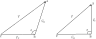
\includegraphics[scale=1]{triangle}
\caption{Triangle Law of Vectors}\label{triangle_pic}
\end{figure}


\textbf{a.} The 2 vectors are in Continuation with each other i.e Head Point of one vector is the Tail Point of the Other Vector. The vector containing the Common point as Tail is called the Leading Vector. The Vector containing the Common Point as Head is called the Trailing Vector.

\textbf{b.} The 2 ectors share a common Tail Point.


\textbf{c.} The 2 vectors share a common Head Point.


Triangular Law of Vector Addition states that If 2 Vectors that are in Continuation ( i.e. Head Point of one Vector is the Tail Point of the Other Vector) are added then the Resultant Vector has the Head Point of the Lead Vector and Tail Point of the Trailing Vector. Since the 2 Vectors and the Resultant Vector form a Triangle, it is know as the Triangular Law of Vector Addition.


\beq
\vec{AC} = \vec{AB} + \vec{BC} = \vec{BC} + \vec{AB}
\eeq


And as per Cosine Law of Triangles


\beq
\vert \vec{AC} \vert = \vert \vec{CA} \vert  = \sqrt{\vert \vec{AB} \vert^2 + \vert \vec{BC} \vert^2 - 
2\vert \vec{AB} \vert \vert \vec{BC} \vert \cos \theta}
\eeq


Triangle Law can be used to Find the Resultant Vector under following conditions

\textbf{a.} Addition of 2 Vectors that are in Continuation with each other: The resultant Vector of addition of 2 given vectors $\vec{AB}$ and $\vec{BC}$ is given as

\beq
\vec{AB} + \vec{BC} = \vec{BC} + \vec{AB} = \vec{AC}
\eeq


\textbf{b.} Subtraction of 2 Vectors that Have a Common Tail Point: The resultant Vector of Subtration of 2 Vectors $\vec{AB}$ and $\vec{CB}$ is given as

\beq
\vec{AB} - \vec{CB} = \vec{AB} + \vec{BC} = \vec{AC} \\
\vec{CB} - \vec{AB} = \vec{CB} + \vec{BA} = \vec{CA}
\eeq


\textbf{c.} Subtraction of 2 Vectors that Have a Common Head Point: The resultant Vector of Subtration of 2 Vectors $AB$ and $AC$ is given as


\beq
\vec{AB} - \vec{AC} = \vec{AB} + \vec{CA} = \vec{CA} + \vec{AB} = \vec{CB} \\
\vec{AC} - \vec{AB} = \vec{AC} + \vec{BA} = \vec{BA} + \vec{AC} = \vec{BC}
\eeq




% =====================================================
% Orthogonal Vector Projection / Rejection
% https://stemandmusic.in/maths/mvt-algebra/vectorPR.php
% =====================================================


Any vector $\vec{V}$ can be represented as a sum of its Projection vector ($\vec{V_{P}}$) and Rejection vector ($\vec{V_{R}}$) on any other vector. That is

\beq
\vec{V} = \vec{V}_{P} + \vec{V}_{V}
\eeq

When the vector $\vec{V}$'s Projection and Rejection vectors are perpendicular to each other then Projection vector $(\vec{V}_{P})$ is also called its Horizontal component $(\vec{V}_{H})$ and Rejection vector $(\vec{V}_{R})$ is also called its Vertical component $(\vec{V}_{V})$.
Hence, any vector $\vec{V}$ can be presented as sum of its Horizontal $(\vec{V}_{H})$ and Vertical
$(\vec{V}_{V})$ components based on any other vector. That is

\beq
\vec{V} = \vec{V}_{H} + \vec{V}_{V}
\eeq

Hence:

\beq \label{rejection_component}
\vec{V}_{V} = \vec{V} - \vec{V}_{H}
\eeq

% https://www.varsitytutors.com/hotmath/hotmath_help/topics/adding-and-subtracting-vectors
%The parallelogram method:

%\begin{figure}[!htbp]
%\centering
%\includegraphics[scale=0.5]{vec_parallelogram}
%\caption{Parallelogram Method}\label{vec_parallelogram_pic}
%\end{figure}


%The triangle method:

%\begin{figure}[!htbp]
%\centering
%\includegraphics[scale=0.5]{vec_triangle}
%\caption{Triangle Method}\label{vec_triangle_pic}
%\end{figure}


%\newpage
%/media/andriy/3TB/InfoA/MathPhys/Basis/Линейная алгебра Антика/mo112.pdf
%https://en.wikipedia.org/wiki/Vector_projection
% https://davidaustinm.github.io/ula/sec-orthogonal-bases.html








\subsection{Orthogonal Scalar Projection}

Definition of the $\cos(\alpha)$ function.

% https://en.wikipedia.org/wiki/Sine_and_cosine

\begin{figure}[!htbp]
\centering
\includegraphics[scale=0.5]{cosine_angle2}
\caption{Definition of the $\cos(\alpha)$ function.}\label{cosine_pic}
\end{figure}


\beq \label{cosine_definition}
\cos(\varphi) = \frac{\text{adjacent}}{\text{hypotenuse}} = \frac{\vert \vec{b} \vert}{\vert \vec{a} \vert}
\eeq

\beq \label{simple_scalar_projection}
\vert \vec{b} \vert = \text{adjacent} = \text{hypotenuse} \cdot \cos(\varphi) =  \vert \vec{a} \vert \cdot \cos(\varphi)
\eeq


\beq 
\vert \vec{c} \vert = \vert \vec{a} \vert \sin \varphi
\eeq


\beq \label{scalar_product_geom}
\vert \vec{a} \vert^{2} = \sqrt{\vert \vec{b} \vert^{2} + \vert \vec{c} \vert^{2} - 2\vert \vec{b} \vert \vert \vec{c} \vert \cos \theta} = \sqrt{\vert \vec{b} \vert^{2} + \vert \vec{c} \vert^{2}}
\eeq

That is why it is easier to choice orthogonal basis for the computations - because the $\cos \theta = 0$ and the formula (\ref{scalar_product_geom}) is simplified.



The $adjacent$ is a scalar projection of $hypotenuse$ onto the direction parallel to the $adjacent$.

% /media/andriy/3TB/InfoA/MathPhys/Basis/Линейная алгебра Антика/mo112.pdf
Let's introduce new notation for a scalar orthogonal projection:

\beq \label{scalar_projection}
\text{Proj}_{\vec{b}}\vec{a} = \vert \vec{a} \vert \cos(\widehat{\vec{b}, \vec{a}})
\eeq 

In the case of figure (\ref{cosine_pic})
\beq
\vert \vec{b} \vert = \text{Proj}_{\vec{b}}\vec{a}
\eeq

- in this case:

\beq
\vert \vec{b} \vert \vert \vec{b} \vert = {\vert \vec{b} \vert}^2 = 
\vert \vec{b} \vert \cdot \text{Proj}_{\vec{b}}\vec{a} = \vert \vec{b} \vert \vert \vec{a} \vert \cos(\widehat{\vec{b}, \vec{a}}) = 
(\vec{b},\vec{a})
\eeq

But this is a special case.

The $\vec{b}$ vector can have arbitrary length but the same direction. In this case:

\begin{figure}[!htbp]
\centering
\includegraphics[scale=0.5]{orth_proj_4}
\caption{Orthogonal Scalar Projection}\label{orth_proj_4}
\end{figure}


\beq \label{geom_dot_product_1}
(\vec{b}, \vec{a}) = 
\vert \vec{b} \vert \cdot \text{Proj}_{\vec{b}}\vec{a} = \vert \vec{b} \vert \vert \vec{a} \vert \cos(\widehat{\vec{b}, \vec{a}})
\neq
{\vert \vec{b} \vert}^2
\eeq


\beq \label{cosine_dot_product}
\cos(\widehat{\vec{b}, \vec{a}}) = \frac{(\vec{b}, \vec{a})}{\vert \vec{b} \vert \vert \vec{a} \vert}
\eeq







%From the (\ref{simple_scalar_projection}) we can see that the $adjacent$ and the $opposite$ can be considered as a coordinates of a vector $hyponetuse$

%Let's introduce some orthogonal coordinate system - $\vec{e}_1$, $\vec{e}_2$, where $\vec{e}_1$ is a unit vector parallel to the $adjacent$ and the  $\vec{e}_2$ is a unit vector parallel to the $opposite$. 

So, in general, in the (\ref{scalar_projection}) we are taking the projection in the direction of $\vec{b}$. And the $\vec{b}$ can have an arbitrary length.
If we take the length of the $\vec{b}$ equals to 1, and denote it as  $\vec{e}_1$ - \textbf{unit vector} collinear with $\vec{b}$ the result will be:

\beq \label{scalar_projection_onto_e1}
\vert \vec{b} \vert = \text{Proj}_{\vec{e}_{1}}\vec{a} = \vert \vec{a} \vert \cos(\widehat{\vec{e}_{1}, \vec{a}})
= \vert \vec{a} \vert \vert \vec{e}_{1} \vert \cos(\widehat{\vec{e}_{1}, \vec{a}})
= (\vec{e}_{1},\vec{a}) = a_{1}
\eeq 



I.e, \textbf{the scalar projection of some vector onto it's first basis vector coincides with it's first coordinate - $\vert \vec{b} \vert = a_{1}$}.

Therefore:

\beq \label{geom_dot_product_2}
(\vec{b}, \vec{a}) = a_1 \vert \vec{b} \vert = (\vec{e}_{1}, \vec{a}) \vert \vec{b} \vert
\eeq

The (\ref{geom_dot_product_1}) and (\ref{geom_dot_product_2}) is a geometrical definition of a dot product.


% https://en.wikipedia.org/wiki/Dot_product#:~:text=Algebraically%2C%20the%20dot%20product%20is,equivalent%20when%20using%20Cartesian%20coordinates.
In multidimensional euclidean space:

\beq \label{vector_in_basis}
\vec{a} = [a_{1}, \cdots , a_{n}] = \sum_{i} a_{i}\vec{e}_{i} \\
\vec{b} = [b_{1}, \cdots , b_{n}] = \sum_{i} b_{i}\vec{e}_{i} \\
\eeq

\beq \label{multi_scalar_projection_onto_e1}
(\vec{e}_{i}, \vec{a}) = \vert \vec{a} \vert \cos (\widehat{\vec{e}_{i}, \vec{a}}) = \vert  \vec{e}_{i} \vert \vert \vec{a} \vert \cos (\varphi_{i}) =  a_{i}
\eeq


The algebraic definition of a dot product is:

\beq \label{dot_prod_algebraic_def}
( \vec{b},\vec{a}) = \sum_{i} b_{i}a_{i} = \sum_{i} a_{i}b_{i}
\eeq

Hence:

\beq \label{dot_prod_geom_algebraic_equivalence}
(\vec{b}, \vec{a}) = \sum_{i} b_{i}a_{i} = \sum_{i} a_{i}b_{i} = 
\sum_{i} \vec{b}_{i} (\vec{e}_{i}, \vec{a}) = 
\sum_{i} \vec{a}_{i} (\vec{e}_{i}, \vec{b})
\eeq

\subsection{Linearity of orthogonal scalar projection} \label{subsection_scalar_projection_linear}

The scalar projection is a linear operation. I.e the projection of the sum of vectors is the same as the sum of the projections, and the scalar factor can be taken out of the brackets:

\beq \label{scalar_projection_linear_1}
\text{Proj}_{\vec{b}}(\vec{a}_{1} + \vec{a}_{2}) =
\text{Proj}_{\vec{b}}(\vec{a}_{1}) +
\text{Proj}_{\vec{b}}(\vec{a}_{2}) 
\eeq

\beq \label{scalar_projection_linear_2}
\text{Proj}_{\vec{b}}(\lambda \vec{a}) = \lambda \text{Proj}_{\vec{b}} \vec{a}
\eeq

% /media/andriy/3TB/InfoA/MathPhys/Basis/Линейная алгебра Антика/mo112.pdf
%\textbf{Proof}.



\subsection{Orthogonal Vector Projection}

The (\ref{scalar_projection}) is a scalar and as we already show, it does not dependent on the length of a $\vec{b}$. To make this quantity directional, we can multiply it by a unit vector $\vec{e}_{1}$

\beq \label{vector_projection}
\overrightarrow{\text{Proj}}_{\vec{b}} \vec{a} = \vert \vec{a} \vert \cos(\widehat{\vec{b}, \vec{a}}) \vec{e}_{1} = a_{1}\vec{e}_{1}
\eeq

Multiplying a vector by a scalar simply scales the vector without changing its direction.

Example:

Let $\vec{u} = [-1,3]$. Find $7\vec{u}$: 

$7 \vec{u} = [-7, 21]$




Since:

\beq
\vec{e}_{1} = \frac{\vec{b}}{\vert \vec{b} \vert} \\
\vec{b} = \vert \vec{b} \vert \vec{e}_{1} = \text{Proj}_{\vec{e}_{1}}\vec{a} \cdot \vec{e}_{1} = 
a_{1}\vec{e}_{1}
\eeq

- then:

\beq \label{vector_projection_2}
\overrightarrow{\text{Proj}}_{\vec{b}} \vec{a} =  \frac{\vert \vec{a} \vert \cos(\widehat{\vec{b}, \vec{a}})}{\vert \vec{b} \vert} \vec{b}
\eeq

- substitute the (\ref{cosine_dot_product}):

\beq \label{vector_projection_3}
\overrightarrow{\text{Proj}}_{\vec{b}} \vec{a} = \frac{(\vec{b}, \vec{a})}{\vert \vec{b} \vert^2} \vec{b}
\eeq

Let's donote it as:

\beq
\overrightarrow{\text{Proj}}_{\vec{b}} \vec{a} = \lambda \vec{b} = \lambda a_{1} \vec{e}_{1} = \lambda  \vert \vec{b} \vert \vec{e}_{1} = \lambda \vec{b}
\eeq

-where:

\beq
\lambda = \frac{\vert \vec{a} \vert \cos(\varphi)}{\vert \vec{b} \vert} = 
\frac{(\vec{b}, \vec{a})}{\vert \vec{b} \vert^2}
\\
\cos(\varphi) = \cos(\widehat{\vec{b}, \vec{a}})
\eeq

The $\lambda$ coefficient is called \textbf{Fourier coefficient.}





\subsection{Properties of a dot product}

In the (\ref{subsection_dot_product}) we already considered some of the properties of the dot product.
Let's consider the properties of the scalar product in more detail.

Let $V$ be a vector space over $\mathbb{R}$.

A dot product $(\cdot, \cdot)$ is a function $V \times V \rightarrow \mathbb{R}$ with the following properties


\textbf{Property 1:} Dot product with itself is non-negative

\beq \label{dot_prod_non_negative}
\forall \vec{a} \in V \\
(\vec{a}, \vec{a}) \geqslant 0
\eeq


We know that the $(\vec{a}, \vec{a}) = \vert \vec{a} \vert^2$ - the lenght of a vector. The length cannot be negative. 


\textbf{Property 2:} Dot product with self is zero iff zero vector

\beq \label{dot_prod_zero_if_zero}
(\vec{a}, \vec{a}) = 0 \Leftrightarrow \vec{a} = 0
\eeq


\textbf{Property 3:} Orthogonality.

If $(\vec{b}, \vec{a}) = 0$ then it can be clearly seen that either $\vec{a}$ or $\vec{b}$ is zero or $\cos(\Theta) = 0 \Rightarrow \Theta = \frac{\pi}{2}$

It suggests that either of the vectors is zero or they are perpendicular to each other.

\textbf{Property 4:} Norm of a vector.

The dot product of a vector to itself is the magnitude squared of the vector i.e.

$(\vec{a}, \vec{a}) = \vert \vec{a} \vert \vert \vec{a} \vert \cos(0) = \vert \vec{a} \vert^2$ which is a square of the length of a vector.


\textbf{Property 5:} Scalar projection.

$a_{b} = \vert \vec{a} \vert \cos(\theta)$ where the $\theta$ is the angle between $\vec{a}$ and $\vec{b}$

In terms of the geometric definition of the dot product, this can be rewritten as

$a_{b} = (\hat{b}, \vec{a})$

where $\hat{b} = \frac{\vec{b}}{\vert \vec{b} \vert}$

The dot product is thus characterized geometrically by

$ (\vec{b}, \vec{a}) = a_{b} \vert \vec{b} \vert = b_{a} \vert \vec{a} \vert $

\textbf{Property 6:} Disctibutive over vector addition.

\beq \label{dot_prod_distributive}
(\vec{a}, \vec{b} + \vec{c}) = (\vec{a}, \vec{b}) + (\vec{a},  \vec{c})
\eeq



\textbf{Property 7:} Dot product is \textbf{symmetric}, i.e - commutative.

\beq \label{dot_prod_symmetry}
(\vec{a}, \vec{b}) = (\vec{b}, \vec{a})
\eeq

This property follows from the geometric (\ref{geom_dot_product_1}) and algebraic (\ref{dot_prod_algebraic_def}) definition of a dot product.

But the \textbf{projections are not symmetric}.



\textbf{Property 8:} Bilinearity. Bilinear means linear in every argument.

\beqn
\forall \vec{a}, \vec{a}, \vec{c} \in V \text{ and } \forall \lambda, \mu \in \mathbb{R}
\eeq

\beq \label{dot_prod_bilinear_1}
(\lambda \vec{a} + \mu \vec{b}, \vec{c}) = \lambda (\vec{a}, \vec{c}) + 
\mu (\vec{b}, \vec{c})
\eeq

\beq \label{dot_prod_bilinear_2}
(\vec{a}, \lambda \vec{b} + \mu \vec{c}) = \lambda (\vec{a}, \vec{b}) + \mu (\vec{a}, \vec{c})
\eeq

The (\ref{dot_prod_bilinear_1}) and the (\ref{dot_prod_bilinear_2}) follows from the linearity of a scalar orthogonal projection - (\ref{scalar_projection_linear_1}) and (\ref{scalar_projection_linear_2})

%/media/andriy/3TB/InfoA/MathPhys/Quantum Mechanic/Quantum Computing/short


% https://math.stackexchange.com/questions/1311394/why-conjugate-when-switching-order-of-inner-product


\textbf{Property 9:} Not associative.

Formally, a binary operation $\ast$ on a set $S$ is called \textbf{associative} if it satisfies the associative law:

\beq \label{associative_law}
\forall x, z, z \text{ in } S \\
(x \ast y) \ast z = x \ast (y \ast x)
\eeq

But because the dot product between a scalar $(\vec{a}, \vec{b})$ and a vector $\vec{c}$ is not defined the associative law is \textbf{ill-defined}.

But the dot product is associative with respect to scalar multiplication $c (\vec{a}, \vec{b}) = 
(c \vec{a}, \vec{b}) = (\vec{a}, c \vec{b})$


% https://en.wikipedia.org/wiki/Dot_product
% https://byjus.com/maths/dot-product-of-two-vectors/
% short/mo112.pdf

\textbf{Property 10:} No cancellation.

Unlike multiplication of ordinary numbers, where if $ab = ac$, then $b$ always equals $c$ unless $a$ is zero, the dot product does not obey the \textbf{cancelation law}.

If $(\vec{a}, \vec{b}) = (\vec{a}, \vec{c})$, then we can write: 
$(\vec{a}, \vec{b} - \vec{c}) = 0$ by the distribution law. The result above says this just means that $\vec{a}$ is perpendicular to $(\vec{b} - \vec{c})$, which still allows $\vec{b} - \vec{c} \neq 0$, and therefore allows $\vec{b} \neq \vec{c}$.


\subsection{Properties of an inner product}

As we already show in the (\ref{subsection_inner_roduct}) for a complex spaces we have to modify the dot product. In this case we also call it \textbf{hermitian product}.

Let's consider this modifications in more details.

\textbf{Property 1:} Symmetric property becomes conjugate-symetric.

The symmetry property (\ref{dot_prod_symmetry}) is no longer met. Indeed for any $\vec{a}$ and $\vec{b}$ in $\mathbb{C}$ so that:

\beq
\vec{a} =
\begin{bmatrix}
a_1 \\ \cdots \\ a_n
\end{bmatrix}
,
\vec{b} =
\begin{bmatrix}
b_1 \\ \cdots \\ b_n
\end{bmatrix}
\eeq

\beq
\bra{\vec{b}}\ket{\vec{a}} \sim (\vec{b}^{\dag}, \vec{a})
\eeq

where the $\vec{b}^{\dag}$ is a transposed vector with complex conjugate components.

The $\dag$ operation - is called \textbf{Conjugate Transpose of a Vector}.

To swap $\vec{a}$ and $\vec{b}$ we have to apply conjugate transpose to both of them.

\beq \label{hermitian_product}
(\vec{b}^{\dag}, \vec{a}) = (\vec{a}^{\dag}, \vec{b})^{\dag}
\eeq

%\beq \label{hermitian_product}
%\bra{\vec{b}}\ket{\vec{a}} \sim (\vec{b}^{\dag}, \vec{a}) = (\vec{a}^{\dag}, \vec{b}^{\dag^{\dag}}) = (\vec{a}^{\dag}, \vec{b})^{\dag} \sim \bra{\vec{a}}\ket{\vec{b}}^{\dag}
%\eeq

% https://math.libretexts.org/Bookshelves/Linear_Algebra/Book%3A_Linear_Algebra_(Schilling_Nachtergaele_and_Lankham)/09%3A_Inner_product_spaces/9.01%3A_Inner_Products
%\beq
%\bra{\vec{a}}\ket{\vec{b}} = \sum_{i} a_{i} \bar{b_{i}}
%\eeq

% https://math.stackexchange.com/questions/1684589/property-of-the-conjugate-transpose-matrix-with-inner-product
%\beq
%\bra{\vec{b}}\ket{\vec{a}} = \sum_{i} \bar{b_{i}} a_{i}
%\eeq

Therefore the hermitian product is conjugate-symmetric, but the dot product is symmetric.


% /media/andriy/3TB/InfoA/MathPhys/Quantum Mechanic/Quantum Computing/short/cqt03.pdf
\textbf{Property 2:} Linear as a function of its second argument. 

\beq \label{inner_prod_similinear}
\bra{\vec{c}} \ket{\alpha \vec{a} + \beta \vec{b} } = \alpha \bra{\vec{c}}\ket{\vec{a}} + \beta \bra{\vec{c}}\ket{\vec{b}}
\eeq

% /media/andriy/3TB/InfoA/MathPhys/Quantum Mechanic/Quantum Computing/short/cqt03.pdf
\textbf{Property 3:} Antilinear function of tis first argument

\beq \label{inner_prod_antilinear}
\bra{ \alpha \vec{a} + \beta \vec{b} } \ket{\vec{c}} = \bar{\alpha}\bra{\vec{a}}\ket{\vec{c}} + \bar{\beta} \bra{\vec{b}}\ket{\vec{c}}
\eeq


\subsection{Outer product}
It is a standard matrix of the vector orthogonal projection.

Let's consider the (\ref{vector_projection_3}) again.

As we remember, in the case of complex space, we have to write it in the form of:

\beq \label{vector_projection_4}
\overrightarrow{\text{Proj}}_{\vec{b}} \vec{a} = \frac{\bra{\vec{b}}\ket{\vec{a}}}{\vert \vec{b} \vert^2} \ket{\vec{b}}
\eeq

- and since the $\bra{\vec{b}}\ket{\vec{a}}$ it is a scalar we can rewrite it as follows:

\beq \label{vector_projection_5}
\overrightarrow{\text{Proj}}_{\vec{b}} \vec{a} = \frac{1}{\vert \vec{b} \vert^2}
\ket{\vec{b}}\bra{\vec{b}}\ket{\vec{a}}
\eeq

Hence, we have a formula:

\beq
\bra{\vec{b}}\ket{\vec{a}}\ket{\vec{b}} = \ket{\vec{b}}\bra{\vec{b}}\ket{\vec{a}}
\eeq

And according to the vector(matrix) multiplication rules the $\ket{\vec{b}}\bra{\vec{b}}$ produces a matrix.

Sometimes, the cross product is denoted as follows $\vec{c} \otimes \vec{b}$, then there is some more general relation:

% /media/andriy/3TB/InfoA/MathPhys/Quantum Mechanic/Quantum Computing/short/The Dirac Representation of the Outer Pro.pdf
\beq \label{outer_product_dot_product}
\left( \vec{c} \otimes \vec{b} \right)\vec{a} = \vec{c} \left( \vec{b} \cdot \vec{a} \right)
\eeq

\textbf{This therefore takes a vector in the $\vec{a}$ direction and gives back one in a $\vec{c}$ direction.}

To proof it just rewrite it in a bra-ket notation.

\beql{
\ket{\vec{c}}\bra{\vec{b}}\ket{\vec{a}} = \ket{\vec{c}}\bra{\vec{b}}\ket{\vec{a}}
}{outer_scalar_rpoduct_relation}

\textbf{If we have an orthonormal basis, $\vec{e}_{i}, i=1...N$, then the outer product
$\vec{e}_{i} \otimes \vec{e}_{j}$ acting on a vector $\vec{a}$ picks out the j-th component of the vector and gives it back in the i-th direction; that is}

\beq \label{outer_product_basis}
\left( \vec{e}_{i} \otimes \vec{e}_{j} \right) \vec{a} =
\vec{e}_{i} \left( \vec{e}_{j} \cdot \vec{a} \right) = a_{j}\vec{e}_{i}
\eeq

The matrix that does this job is one with 1 in the j-th row and i-th columnt and 0 everywhere else.

\subsection{Completeness Relation}

% short/qmech1.pdf
Acctording to the (\ref{2d_comp_basis}) and the (\ref{vector_in_basis}) arbitrary state $\psi$
can be written as linear superposition of basis vectors (in computational basis, as linear combination of eigenkets)

\beq \label{vector_again}
\ket{\psi} = \sum_{i}a_{i}\ket{e_{i}}
\eeq

Taking inner product with $\bra{e_{j}}$, and using the ortho normality of $\ket{e_{i}}$, we have


\beq \label{multi_scalar_projection_onto_e1_again}
\bra{e_{j}}\ket{\psi} = \sum_{i} \bra{e_{j}} a_{i} \ket{e_{i}} =
\sum_{i} a_{i} \bra{e_{j}}\ket{e_{i}} =
\sum_{i} a_{i}\delta_{ij} = a_{j}
\eeq

For 2D spaces this coincides with (\ref{scalar_projection_onto_e1}) and for multidimensional spaces it coincides with (\ref{multi_scalar_projection_onto_e1})

Substituting back in Eq. (\ref{vector_again}) we have

\beq \label{vector_by_outer_product}
\ket{\psi} = 
\sum_{i} \bra{e_{i}} \ket{\psi} \ket{e_{i}} = 
\left( \sum_{i} \ket{e_{i}} \bra{e_{i}} \right) \ket{\psi}
\eeq




Similarly we can write any matrix as an outer product operator


\beq \label{matrix_as_outer_product}
A = \sum_{i,j=1}^{N} A_{ij}e_{i} \otimes e_{j} = 
\sum_{i,j=1}^{N} A_{ij} \ket{e_{i}}\bra{e_{j}} = 
\sum_{i,j=1}^{N} \ket{e_{i}} A_{ij} \bra{e_{j}}
\eeq

\beq \label{identity_matrix}
\mathbb{1} = \sum_{i,j=1}^{N} \ket{e_{i}} \delta_{ij}\bra{e_{j}} = 
\sum_{i=1}^{N} \ket{e_{i}}\bra{e_{i}}
\eeq

- the (\ref{identity_matrix}) is also called \textbf{resolution of identity.}

% lecture_3_453.pdf
- this can be inserted in any expression without affecting its value, for example:

\beql{
\bra{\phi}\ket{\psi} = \bra{\phi}\sum_{i\in N} \ket{e_i}\bra{e_i}\ket{\psi} =
\bra{\phi}\sum_{i\in N} \ket{e_i}\bra{e_i} \sum_{j\in N} \ket{e_j}\bra{e_j} \ket{\psi} = 
\bra{\phi}\ket{e_i}\bra{e_i}\ket{e_j}\bra{e_j}\ket{\psi}
}{double_res_of_id}


Hence the (\ref{matrix_as_outer_product}) can be rewritten in the form of:

\beql{
& A = \mathbb{1} A \mathbb{1} =
\left( \sum_i \ket{e_i}\bra{e_i} \right)
A
\left( \sum_j \ket{e_j}\bra{e_j} \right) = 
\sum_{ij} \ket{e_i}\bra{e_i} A \ket{e_j}\bra{e_j} = \sum_{ij}^{N} \ket{e_{i}} A_{ij} \bra{e_{j}} \\
& A_{ij} = \bra{e_i} A \ket{e_j} \;\;\; - \text{just a number}
}{matrix_as_outer_product_2}


%/media/andriy/3TB/InfoA/MathPhys/Quantum Mechanic/Quantum Computing/short/Inner Product Spaces and Orthogonality.pdf



%-----------------------------------------------

\textbf{In the case of quantum mechanics}, state vectors are normilized i.e $\vert \phi \vert^2 = 1$

Hence, according to the (\ref{vector_projection_5}):

\beq \label{quantum_projection}
\overrightarrow{\text{Proj}}_{\phi} \psi =
\ket{\phi}\bra{\phi}\ket{\psi}
\eeq

%https://www.youtube.com/watch?v=GkKLBC1eoUc

% Projection
% https://ximera.osu.edu/mooculus/calculus2/dotProducts/digInProjections2E

%/media/andriy/3TB/InfoA/MathPhys/Quantum Mechanic/Quantum Computing/short/Inner Product Spaces and Orthogonality.pdf

% https://www.youtube.com/watch?v=_Z_tCGZ8KBo
% Quantum Mechanics - 5 - Outer Products and Projection Operators.mp4


In general, product of ket $\ket{\phi}$ and bra $\bra{\psi}$, is called an \textbf{outer product}.

An outer product, producing a matrix. Example:

\renewcommand*{\arraystretch}{2}
%\setlength{\arraycolsep}{5pt}
\beq \label{outer_product_example}
\ket{\phi}\bra{\psi} = \left| \phi \psi \right| = 
\begin{bmatrix}
-\frac{-4}{5} \\ \frac{3}{5}
\end{bmatrix}
\begin{bmatrix}
\frac{1}{2} & \frac{\sqrt{3}}{2}
\end{bmatrix} = 
\begin{bmatrix}
-\frac{4}{10} & -\frac{4\sqrt{3}}{10} \\
\frac{3}{10} & \frac{3\sqrt{3}}{10}
\end{bmatrix}
\eeq


% https://chem.libretexts.org/Bookshelves/Physical_and_Theoretical_Chemistry_Textbook_Maps/Time_Dependent_Quantum_Mechanics_and_Spectroscopy_(Tokmakoff)/01%3A_Overview_of_Time-Independent_Quantum_Mechanics/1.02%3A_Matrix_Mechanics
%The outer product  |i⟩⟨i|
%  is known as a projection operator because it can be used to project the wavefunction of the system onto the  ith
%  eigenstate of the system as  |i⟩⟨i∣Ψ⟩=ci|i⟩
% . Furthermore, if we sum projection operators over the complete basis set, we obtain an identity operator



% /media/andriy/3TB/InfoA/MathPhys/Quantum Mechanic/Quantum Computing/short/youtube/[The Materials Research Society Series] Ray LaPierre - Introduction to Quantum Computing (2021, Springer) - libgen.li.pdf
An outer product $\ket{\phi}\bra{\phi}$ is also known as a \textbf{projection operator}. Projection operator it is a standard matrix of orthogonal projection.
% ?They \textbf{project} some vector $\ket{\psi}$ onto the vector $\ket{\phi}$?.



According to the (\ref{rejection_component}), (\ref{vector_projection_5}) and Fig(\ref{cosine_pic}):

\beq \label{vector_rejection}
\overrightarrow{\text{Proj}}_{\vec{c}} \vec{a} = \vec{a} - \overrightarrow{\text{Proj}}_{\vec{b}} \vec{a} = \left( I - \frac{1}{\vert \vec{b} \vert^2} \ket{\vec{b}} \bra{\vec{b}} \right) \ket{\vec{a}}
\eeq


The (\ref{vector_rejection}) is called \textbf{vector rejection}.



% https://en.wikipedia.org/wiki/Vector_projection
In two dimensions, the scalar rejection is equivalent to the projection of $\vec{a}$ onto $\vec{b}^{\perp} = (-\vec{b}_{y}, \vec{b}_{x})$, which is $\vec{b} = (\vec{b}_{x}, \vec{b}_{y})$ rotated $90^{\circ}$ to the left,

Hence

\beq
\vert \vec{c} \vert = \vert \vec{a} \vert \sin \theta = \frac{(\vec{a},\vec{b}^{\perp})}{\vert \vec{b} \vert} = 
\frac{\vec{a}_{y}\vec{b}_{x} - \vec{a}_{x}\vec{b}_{y}}{\vert \vec{b} \vert}
\eeq

Let's return to the orthogonal projection in multidimensional space:

% Линейная алгебра Антика/LinearAlgebraDoneOpenly.pdf

\textbf{Theorem (Parseval's Identity.)} Let $S = \left\lbrace \vec{v}_{1}, \cdots, \vec{v}_{p} \right\rbrace \subseteq F^{n}$ be an orthogonal subset. If $\vec{y}$ is a linear combination of the vectors in $S$, that is,

\beq
\vec{y} = c_{1}\vec{v}_{1} + c_{2}\vec{v}_{2} + \cdots + c_{p}\vec{v}_{p}
\eeq

then

\beq
c_{i} = \frac{\vec{v}_{i} \cdot \vec{y}}{\vec{v}_{i} \cdot \vec{v}_{i}}
\eeq

-is called \textbf{Fourier coefficients.}


\textbf{Proof.} Taking the dot product, we get

\beq
\vec{v}_{i} \cdot \vec{y} = \vec{v}_{i} (c_{1}\vec{v}_{1} + c_{2}\vec{v}_{2 + \cdots + c_{p}\vec{v}_{p}}) = c_{i}(\vec{v}_{i}, \vec{v}_{i})
\eeq


Since $\vec{v}_{i} \cdot \vec{v}_{i} \neq 0$, dividing both sides by $\vec{v}_{i} \cdot \vec{v}_{i}$ gives the formula.






\textbf{Example of projection operator.}


\beq
\hat{\text{P}}\vec{v} = 
\left[
	\begin{array}{c c c}
		1 & 0 & 0 \\
		0 & 1 & 0 \\
		0 & 0 & 0 \\
	\end{array}
\right]
\left[
	\begin{array}{c}
		x \\
		y \\
		z
	\end{array}
\right] = 
\left[
	\begin{array}{c}
		x \\
		y \\
		0
	\end{array}
\right]
\eeq

\newpage

Thus, the action of this matrix on an arbitrary vector is

\beqn
P
\left[
	\begin{array}{c}
		x \\
		y \\
		z
	\end{array}
\right]
=
\left[
	\begin{array}{c}
		x \\
		y \\
		0
	\end{array}
\right]
\eeq



\begin{figure}[!htbp]
\centering
\includegraphics[scale=1]{simple_projection_pic}
\caption{Orthogonal projection of a vector onto the plane}\label{simple_projection_pic}
\end{figure}



\textbf{Example.} Find the linear mapping from $\mathbb{R}^{3}$ to $\mathbb{R}^{3}$ that is a the orthogonal projection of $\mathbb{R}^{3}$ onto the plane $x_{1} + x_{2} + x_{3} = 0$

To find the orthogonal projection of $\mathbb{R}^{3}$ onto the subspace $\vec{v}^{\perp}$, where $\vec{v} = [1,1,1]^{T}$, we find the following orthogonal projection



\beqn
\text{Proj}_{\vec{v}}(\vec{y}) = \left( \frac{\vec{v} \cdot \vec{y}}{\vec{v} \cdot \vec{v}} \right)
\vec{v} = \frac{y_{1} + y_{2} + y_{3}}{3}
\begin{bmatrix}
1 \\
1 \\
1
\end{bmatrix} = \frac{1}{3}
\begin{bmatrix}
1 & 1 & 1 \\
1 & 1 & 1 \\
1 & 1 & 1
\end{bmatrix}
\begin{bmatrix}
y_{1} \\
y_{2} \\
y_{3}
\end{bmatrix}
\eeq


Then the orthogonal projection of $\vec{y}$ onto $\vec{v}^{\perp}$, according to (\ref{rejection_component}) is given by


\beqn
\text{Proj}_{\vec{v}}\vec{y} = \vec{y} - \text{Proj}_{v}(\vec{y}) = 
\left( I - \frac{1}{\vec{v} \cdot \vec{v}} \vec{v} \vec{v}^{T} \right) \vec{y} = 
\frac{1}{3}
\begin{bmatrix}
2  & -1 & -1 \\
-1 & 2  & -1 \\
-1 & -1 & 2
\end{bmatrix}
\begin{bmatrix}
y_{1} \\ y_{2} \\ y_{3}
\end{bmatrix}
\eeq

% https://www.maplesoft.com/support/help/maple/view.aspx?path=MathApps%2FProjectionOfVectorOntoPlane
I.e. the projection of $\vec{y}$ \textbf{onto a plane} can be calculated by substracting the component $\text{Proj}_{v}(\vec{y})$ that is orthogonal to the plane from $\vec{y}$.

Let $W$ be a subspace of $V$, and let $\vec{v}_{1}, \vec{v}_{2}, \cdots , \vec{v}_{k}$ be an orthogonal basis of $W$. We want to decompose an arbitrary vector $\vec{v} \in V$ into the form
\beqn
\vec{y} = \vec{w} + \vec{z}
\eeq

with $\vec{w} \in W$ and $\vec{z} \in W^{\perp}$. Then there exist scalars $\alpha_{1}, \alpha_{2}, \cdots , \alpha_{k}$ such that

\beqn
\hat{\vec{y}} = \alpha_{1}\vec{v}_{1} + \alpha_{2}\vec{v}_{2} + \cdots + \alpha_{k}\vec{v}_{k}
\eeq

Since $\vec{z} \perp \vec{v}_{1}, \vec{z} \perp \vec{v}_{2}, \cdots, \vec{z} \perp \vec{v}_{k}$, we have

\beqn
(\vec{v}_{i}, \vec{y}) = (\vec{v}_{i}, \alpha_{1}\vec{v}_{1} + \cdots + \alpha_{k}\vec{v}_{k} + \vec{z} ) = \alpha_{i}(\vec{v}_{i}, \vec{v}_{i})
\eeq

Then

\beqn
\alpha_{i} = \frac{\vec{v}_{i} \cdot \vec{y}}{\vec{v}_{i} \cdot \vec{v}_{i}}, \text{ } 1 \leq i \leq k.
\eeq



We thus define

\beqn
\text{Proj}_{W}(\vec{y}) = 
\frac{\vec{v}_{1} \cdot \vec{y}}{\vec{v}_{1} \cdot \vec{v}_{1}}\vec{v}_{1} + 
\frac{\vec{v}_{2} \cdot \vec{y}}{\vec{v}_{2} \cdot \vec{v}_{2}}\vec{v}_{2} +
\cdots + 
\frac{\vec{v}_{k} \cdot \vec{y}}{\vec{v}_{k} \cdot \vec{v}_{k}}\vec{v}_{k},
\eeq

called the \textbf{orthogonal projection of} $\vec{v}$ \textbf{along} $W$. The linear transformation
is called the \textbf{orthogonal projection of} $V$ \textbf{onto} $W$.


\textbf{Theorem}. Let $V$ be an n-dimensional inner product space. Let $W$ be a subspace with an orthogonal basis $\mathcal{B} = \left\lbrace \vec{v}_{1}, \vec{v}_{2}, \cdots, \vec{v}_{k} \right\rbrace $. Then for any $\vec{y} \in V$

\beqn
\text{Proj}_{W}(\vec{y}) = 
\frac{\vec{v}_{1} \cdot \vec{y}}{\vec{v}_{1} \cdot \vec{v}_{1}}\vec{v}_{1} + 
\frac{\vec{v}_{2} \cdot \vec{y}}{\vec{v}_{2} \cdot \vec{v}_{2}}\vec{v}_{2} + 
\cdots +
\frac{\vec{v}_{k} \cdot \vec{y}}{\vec{v}_{k} \cdot \vec{v}_{1}}\vec{v}_{k}
\eeq


\beqn
\text{Proj}_{W^{\perp}} (\vec{y}) = \vec{y} - \text{Proj}_{W}(\vec{y})
\eeq


\textbf{In particular, if $\mathcal{B}$, is an orthonormal basis of $W$, then}

\beqn
\text{Proj}_{W}(\vec{y}) = 
(\vec{v}_{1} \cdot \vec{y})\vec{v}_{1} + 
(\vec{v}_{2} \cdot \vec{y})\vec{v}_{2} + 
\cdots + 
(\vec{v}_{k} \cdot \vec{y})\vec{v}_{k}
\eeq



%Inner Product Spaces and Orthogonality.pdf
\textbf{Proposition} Let $W$ be a subspace of $\mathbb{R}^{n}$. Len $U = [\vec{u}_{1}, \vec{u}_{2}, \cdots, \vec{u}_{k}]$ be an $n \times k$ matrix, whose columns form an orthonormal basis of $W$. Then the orhtogonal projection $\text{Proj}_{W}: \mathbb{R}^{n} \rightarrow \mathbb{R}^{n}$ is given by

\beqn
\text{Proj}_{W}(\vec{y}) = UU^{T}\vec{y}
\eeq


\textbf{Proof}. For any $\vec{y} \in \mathbb{R}^n$, we have

\beqn
\text{Proj}_{W}(\vec{y}) = 
(\vec{v}_{1} \cdot \vec{y})\vec{v}_{1} + 
(\vec{v}_{2} \cdot \vec{y})\vec{v}_{2} + 
\cdots + 
(\vec{v}_{k} \cdot \vec{y})\vec{v}_{k}
\eeq

Note that

\beqn
U^{T}\vec{y} =
\begin{bmatrix}
\vec{u}_{1}^{T} \\ \vec{u}_{2}^{T} \\ \vdots \\ \vec{u}_{k}^{T}
\end{bmatrix} \vec{y} = 
\begin{bmatrix}
\vec{u}_{1}^{T}\vec{y} \\ \vec{u}_{2}^{T}\vec{y} \\ \vdots \\ \vec{u}_{k}^{T}\vec{y}
\end{bmatrix} = 
\begin{bmatrix}
\vec{u}_{1} \cdot \vec{y} \\ \vec{u}_{2} \cdot \vec{y} \\ \vdots \\ \vec{u}_{k} \cdot \vec{y}
\end{bmatrix}
\eeq

Then

\beqn
UU^{T}\vec{y} = \left[  \vec{u}_{1}, \vec{u}_{2}, \cdots , \vec{u}_{k}  \right] 
\begin{bmatrix}
\vec{u_{1} \cdot \vec{y}} \\
\vec{u_{2} \cdot \vec{y}} \\
\vdots \\
\vec{u_{k} \cdot \vec{y}}
\end{bmatrix} = 
\text{Proj}_{W}(\vec{y})
\eeq

\textbf{Example.} Find the orthogonal projection

\beqn
\text{Proj}_{W}: \mathbb{R}^{3} \rightarrow \mathbb{R}^3
\eeq

where $W$ is the plane $x_{1} + x_{2} + x_{3} = 0$

By inspection, the following two vectors

\beqn
\vec{v}_{1} =
\begin{bmatrix}
1 \\ -1 \\ 0
\end{bmatrix} \text{ and } \vec{v}_{2}
\begin{bmatrix}
1 \\ 1 \\ -2
\end{bmatrix}
\eeq

form an orthogonal basis of $W$. Then

\beqn
\text{Proj}_{W}(\vec{y}) = 
\frac{\vec{v}_{1} \cdot \vec{y}}{\vec{v}_{1} \cdot \vec{v}_{1}}\vec{v}_{1} + 
\frac{\vec{v}_{2} \cdot \vec{y}}{\vec{v}_{2} \cdot \vec{v}_{2}}\vec{v}_{2} = \\
\frac{y_{1} - y_{2}}{2}
\begin{bmatrix}
1 \\ -1 \\ 0 
\end{bmatrix}
+ \frac{y_{1} + y_{2} - 2y_{3}}{6}
\begin{bmatrix}
1 \\ 1 \\ -2
\end{bmatrix} = \\ 
\frac{1}{3}
\begin{bmatrix}
2   & -1   & -1 \\
-1  & 2    & -1 \\
-1  &-1    & 2
\end{bmatrix}
\begin{bmatrix}
y_{1} \\
y_{2} \\
y_{3}
\end{bmatrix}
\eeq

% Inner Product Spaces and Orthogonality.pdf
\textbf{Example}. Find the standard matrix of the orthogonal projection

\beqn
\text{Proj}_{W} : \mathbb{R}^{3} \leftarrow \mathbb{R}^{3}
\eeq

where

\beqn
W = \text{Span} \left\lbrace 
\begin{bmatrix}
1 \\ 1 \\ 1
\end{bmatrix}, 
\begin{bmatrix}
1 \\ -1 \\ 0
\end{bmatrix}
\right\rbrace
\eeq

The following two vectors

\beqn
\vec{u_{1}} = \begin{bmatrix}
1/\sqrt{3} \\ 1/\sqrt{3} \\ 1/\sqrt{3}
\end{bmatrix}, \;\;\;
\vec{u_{2}} = \begin{bmatrix}
1/\sqrt{2} \\ -1/\sqrt{2} \\ 0
\end{bmatrix}
\eeq

form of an orthonormal basis of $W$. Then the standard matrix of $\text{Proj}_{W}$ is the product

\beqn
\begin{bmatrix}
1/\sqrt{3} & 1/\sqrt{2} \\
1/\sqrt{3} & 1/\sqrt{2} \\
1/\sqrt{3} & 0
\end{bmatrix}
\begin{bmatrix}
1/\sqrt{3} & 1/\sqrt{3} & 1/\sqrt{3} \\
1/\sqrt{2} & -1/\sqrt{2} & 0
\end{bmatrix}
\eeq

which results the matrix

\beqn
\begin{bmatrix}
5/6   & -1/6   &   1/3 \\
-1/6  & 5/6    &   1/3 \\
1/3   & 1/3    &   1/3
\end{bmatrix}
\eeq

% Inner Product Spaces and Orthogonality.pdf
Alternatively the matrix can be found by computing the orthogonal projection:

\beqnl{
& \text{Proj}_{W}(\vec{y}) = 
\frac{ y_{1} + y_{2} + y_{3} }{3} \begin{bmatrix} 1\\ 1\\ 1\end{bmatrix} +
\frac{ y_{1} - y_{2} }{2} \begin{bmatrix} 1\\ -1\\ 0\end{bmatrix} = \\
& = \frac{1}{6}\begin{bmatrix}
5y_1 - y_2 + 2y_3 \\
-y_1 - 5y_2 + 2y_3 \\
2y_1 - 2y_2 + 2y_3
\end{bmatrix} =
\begin{bmatrix}
5/6   & -1/6   &   1/3 \\
-1/6  & 5/6    &   1/3 \\
1/3   & 1/3    &   1/3
\end{bmatrix} \begin{bmatrix}
y_1 \\ y_2 \\ y_3
\end{bmatrix}
}





%Quantum Mechanics - 5 - Outer Products and Projection Operators.mp4
\textbf{Example.}

Let's consider the state
\beqn
\ket{\psi} = \alpha \ket{\phi_{1}} + \beta \ket{\phi_{2}}, 
\;\;\; \text{ where } \ket{\phi_{1}}, \ket{\phi_{2}} \text{ forms an orthonormal basis}
\eeq

- we want to decompose this state into a set of basis vectors. There is some experiment that define that basis states (Stern–Gerlach experiment, spectroscopy experiment, etc.)

Let's get the $\alpha$ coefficient.
Let's muliply both sides of $\ket{\psi}$ by $\bra{\phi_{1}}$

\beqn
\bra{\phi_{1}} \ket{\psi} = \alpha \bra{\phi_{1}}\ket{\phi_{1}} + \beta \bra{\phi_{1}}\ket{\phi_{2}}
\eeq

-then

\beqnl{
& \bra{\phi_{1}}\ket{\phi_{1}} = 1 \;\;\;\; \text{due to orthonormality} \\
& \bra{\phi_{1}}\ket{\phi_{2}} = 0 \;\;\;\; \text{due to orthogonality}
}

- then

\beqnl{
& \alpha = \bra{\phi_{1}} \ket{\psi}
}

Hence, we can rewrite the $\ket{\psi}$ state without $\alpha$ and $\beta$ coefficients:

\beqnl{
& \ket{\psi} = \bra{\phi_{1}}\ket{\psi}\ket{\phi_{1}} + \bra{\phi_{2}}\ket{\psi}\ket{\phi_{2}} = \\
& \ket{\phi_{1}}\bra{\phi_{1}}\ket{\psi} + \ket{\phi_{2}}\bra{\phi_{2}}\ket{\psi} = \\
& \left[ \ket{\phi_{1}}\bra{\phi_{1}} +   \ket{\phi_{2}}\bra{\phi_{2}} \right] \ket{\psi}
}

- i.e, the $\left[ \ket{\phi_{1}}\bra{\phi_{1}} +   \ket{\phi_{2}}\bra{\phi_{2}} \right] = \mathbb{1}$, it is an idendity matrix.

And in general:

\beq \label{completeness1}
\sum_{i} \ket{\phi_{i}}\bra{\phi_{i}} = \mathbb{1}
\eeq

and according to the (\ref{quantum_projection}), the $\ket{\phi_{i}}\bra{\phi_{i}}$ it is a projection operator. It projects the $\ket{\psi}$ state, onto the $\ket{\phi}$ state.

The (\ref{completeness1}) is called \textbf{Completeness Relation}. 


\textbf{Example.}

Let's go back to a two level system - "spin up" and "spin down"

\beqn
\ket{\psi} = \frac{3}{5}\ket{\uparrow} + \frac{4}{5}\ket{\downarrow}
\eeq

And let's introduce the notation for the projection operator: $\hat{P}_{\uparrow} \equiv \ket{\uparrow}\bra{\uparrow}$

- according to the orthogonality and orthonormality (\ref{spin_up_down}):

\beql{
\hat{P}_{\uparrow}\ket{\psi} = \ket{\uparrow}\bra{\uparrow}
\left( \frac{3}{5}\ket{\uparrow} + \frac{4}{5}\ket{\downarrow} \right) = \ket{\uparrow}\frac{3}{5}
}{projection_experiment}

- it is a projection of $\ket{\psi}$ onto the $\ket{\uparrow}$, but it is not normizied vector.

The general case of the (\ref{projection_experiment}) is: 

%/media/andriy/3TB/InfoA/MathPhys/Quantum Mechanic/Quantum Computing/short/Measurement/physics.mq.edu.au/Chapter11.pdf
\beql{
& \hat{P}_n \ket{\varphi_m} = \delta_{nm} \ket{\varphi_n} \\
& \hat{P}_n\ket{\psi} = \hat{P}_n \sum_m \ket{\varphi_m}\bra{\varphi_m}\ket{\psi} = 
\sum_m \hat{P} \ket{\varphi_m}\bra{\varphi_m} \ket{\psi} \\
& = \sum_m \delta_{nm}\ket{\varphi_m}\bra{\varphi_m} \ket{\psi} = \ket{\varphi_n}\bra{\varphi_n}\ket{\psi}
}{general_projection_experiment}



\textbf{Important}. The result of a projection operator, in general is not normilized state. There can be cases when you project a pure state onto a pure state, then the result can be a normilized state, but not always.









By the definition, a projection $\hat{P}$ is \textbf{idempotent} (i.e. $\hat{P}^{2} = \hat{P}$)
% https://math.stackexchange.com/questions/1574758/prove-that-the-orthogonal-projection-operator-is-idempotent

%/media/andriy/3TB/InfoA/MathPhys/Quantum Mechanic/Quantum Computing/short/Measurement/physics.mq.edu.au/Chapter11.pdf
\beqnl{
\hat{P}^2_n \ket{\varphi_m} = \hat{P}_n \lbrace \hat{P}_n \ket{\varphi_m} \rbrace = 
\delta_{nm} \hat{P}_n \ket{\varphi_m} = \delta^2_{nm} \ket{\varphi_m}   
}


% https://en.wikipedia.org/wiki/Self-adjoint_operator
% https://www.cfm.brown.edu/people/dobrush/am34/MuPad/projection.html
A projection is orthogonal if and only if it is self-adjoint.


\subsection{Projection matrix idempotence}

Let's denote a projection as $\hat{P}$.

\textbf{Definition}. Let $\hat{P}: F^n \rightarrow F^n $ be a linear transformation. We say that $\hat{P}$ is a \textbf{projection} if $\hat{P} \circ \hat{P} = \hat{P} $


Let $A$ be the standsrd matrix of $\hat{P}$. Then the property that $\hat{P} \circ \hat{P} = \hat{P}$ translate to mean that $A^2 = A$. Any matrix (necessarily a square) which satisfies this identity is called an \textbf{idempotent} matrix and is necessarily the standard matrox of a projection.

Let $\vec{x} \in F^n$. Then $\vec{y} = \hat{P}(\vec{x})$ is an arbitrary element of the range of $\hat{P}$. By definition, we have that

\beq \label{projection_idempotent_1}
\hat{P}(\vec{y}) = \hat{P}(\hat{P}(\vec{x})) = \hat{P} \circ \hat{P}(\vec{x}) = \hat{P}(\vec{x}) = \vec{y},
\eeq

that is, a projection is exactly a linear transformation that fixes its image. Essentially this means that while some of the coordinates of $\vec{x}$ are unaltered the other coordinates are forgotten.


\begin{multicols}{2}
Any point already on the $x$-axis has the form $(x,0)$ and is unaffected by the projection.

\vfill
\columnbreak
        \begin{minipage}{\linewidth}
            \centering
            \includegraphics[width=\linewidth]{projection_idempotence}
        \end{minipage}
\end{multicols}


\textbf{Example.} For example, the matices

\beqn
\begin{bmatrix}
1 & 0 \\
0 & 0
\end{bmatrix}, \;\;
\begin{bmatrix}
0 & 0 & 0 \\
0 & 1 & 0 \\
0 & 0 & 0 \\
\end{bmatrix}, \;\;
\begin{bmatrix}
1 & 0 & 0 \\
0 & 1 & 0 \\
0 & 0 & 0 \\
\end{bmatrix}
\eeq

are easily to seen to be idempotent matrices and hence corresponds to projections.

The first matrix is projection in $\mathbb{R}^3$ onto the $x$-axis where the $y$-coordinate is forgotten and replaced with $0$. Any point already on the $x$-axis has the form $(x,0)$ and is unaffected by the projection.

The second matrix is a projection in $\mathbb{R}^3$ onto $y$-axis, where the $x$- and $z$-coordinates are discarded.

The third matrix is a projection in $\mathbb{R}^3$ onto the $xy$-plane, where the $z$-coordinate is the inly information forgotten.


\textbf{Example.}

Find a standard matrix of orthogonal projection of $\mathbb{R}^{2}$ onto the line spanned by 
$(2,-1)$, that is, the line $y = -1/2x$.

A norm of the $\begin{bmatrix} 2 \\ -1 \end{bmatrix}$ vector is $1/\sqrt{5}$. Therefore we have next matrix of orthogonal projection onto the line $y = -1/2x$:

\beqnl{
& \vec{u} \otimes \vec{u} = 
\frac{1}{\sqrt{5}}\begin{bmatrix} 2 \\ -1 \end{bmatrix}
\otimes
\frac{1}{\sqrt{5}}\begin{bmatrix} 2 & -1 \end{bmatrix} = 
\begin{bmatrix}
0.8944 \\ -0.4472
\end{bmatrix}\begin{bmatrix}
0.8944 & -0.4472
\end{bmatrix} = \\
& = \begin{bmatrix}
0.8 & -0.4 \\
-0.4 & 0.2
\end{bmatrix}
}


Let's check that it is idempotent:

\beqn
\begin{bmatrix}
0.8 & -0.4 \\
-0.4 & 0.2
\end{bmatrix}
\begin{bmatrix}
0.8 & -0.4 \\
0.4 & 0.2
\end{bmatrix} = 
\begin{bmatrix}
0.8 & -0.4 \\
-0.4 & 0.2
\end{bmatrix}
\eeq

Let's try to project a $\begin{bmatrix} 2 \\ 2 \end{bmatrix}$ vector:

\beqn
\begin{bmatrix}
0.8 & -0.4 \\
-0.4 & 0.2
\end{bmatrix} \begin{bmatrix}
2 \\ 2
\end{bmatrix} = \begin{bmatrix}
0.8 & -0.4
\end{bmatrix}
\eeq

If you draw a plot you will see it - it is an orthogonal projection.


% LinearAlgebraDoneOpenly.pdf
\textbf{Definition} Let $A$ be an $n \times n$ matrix. We say that $A$ is \textbf{nilpotent} if $A^n = 0$, the zero matrix.

\textbf{Theorem} Let $\vec{u}, \vec{v} \in F^n$ such that $\vec{u}$ and $\vec{v}$ are orthogonal. Then $A = \vec{u} \otimes \vec{v}$ is a nilpotent matrix.

\textbf{Theorem}. All strictly triangular matrices are nilponent.



\subsection{Gram-Schmidt process.}
% Inner Product Spaces and Orthogonality.pdf
Let $W$ be a subspace of an inner product space $V$. Let 
$\mathcal{B} = \left\lbrace \vec{v_{1}}, \vec{v_{2}}, \cdots ,\vec{v_{k}} \right\rbrace $ be a basis of $
W$, not necessarily orthogonal. 

An orthogonal basis $\mathcal{B'}$ may be constructed from $\mathcal{B}$ as follows

\beql{
& \vec{w_{1}} = \vec{v_{1}},                                    \;\;\;\;\;\;\;\;\;\;\;\;\;\;\;\;\;\;\;\;\;\;\;\;\;\;\;\;\;\; W_{1} = \text{Span}\left\lbrace \vec{w_{1}} \right\rbrace \\
& \vec{w_{2}} = \vec{v_{2}} - \text{Proj}_{W_{1}}(\vec{v}_{2}), \;\;\;\;\;\;\;\;\;									               W_{2} = \text{Span}\left\lbrace \vec{w_{1}},  \vec{w_{2}} \right\rbrace \\
& \vec{w_{3}} = \vec{v_{3}} - \text{Proj}_{W_{2}}(\vec{v}_{3}), \;\;\;\;\;\;\;\;\;                                           W_{3} = \text{Span}\left\lbrace \vec{w_{1}},  \vec{w_{2}},  \vec{w_{3}} \right\rbrace \\
& \vdots \\
& \vec{w}_{k-1} = \vec{v}_{k-1} - \text{Proj}_{W_{k-1}}(\vec{v_{k-1}}), \;\;\; W_{k-1 = \text{Span}}\left\lbrace \vec{w_{1}}, \cdots \vec{w}_{k-1} \right\rbrace , \\
& \vec{w}_{k} = \vec{v}_{k} - \text{Proj}_{W_{k-1}}(\vec{v}_{k})
}{gram_shmidt1}

More precisely

\beql{
& \vec{w}_{1} = \vec{v}_{1}, \\
& \vec{w}_{2} = \vec{v}_{2} - \frac{\bra{\vec{w}_{1}}\ket{\vec{v}_{2}}}{\bra{\vec{w}_{1}}\ket{\vec{w}_{1}}} \vec{w}_{1} \\
& \vec{w}_{3} = \vec{v}_{3} - \frac{\bra{\vec{w}_{1}}\ket{\vec{v}_{3}}}{\bra{\vec{w}_{1}}\ket{\vec{w}_{1}}}\vec{w}_{1} - \frac{\bra{\vec{w}_{2}}\ket{\vec{v}_{3}}}{\bra{\vec{w}_{2}}\ket{\vec{w}_{2}}}\vec{w}_{2} \\
& \vdots \\
& \vec{w}_{3} = \vec{v}_{3} - \frac{\bra{\vec{w}_{1}}\ket{\vec{v}_{3}}}{\bra{\vec{w}_{1}}\ket{\vec{w}_{1}}}\vec{w}_{1} - \frac{\bra{\vec{w}_{2}}\ket{\vec{v}_{3}}}{\bra{\vec{w}_{2}}\ket{\vec{w}_{2}}}\vec{w}_{2} - \cdots -
\frac{\bra{\vec{w}_{k-1}}\ket{\vec{v}_{k}}}{\bra{\vec{w}_{k-1}}\ket{\vec{w}_{k-1}}}\vec{w}_{k-1}
}{gram_shmidt2}

The method of constructing the orthogonal vector $\vec{w}_{1}, \vec{w}_{2}, \cdots, \vec{w}_{k}$ is known as the \textbf{Gram-Schmidt process}.



\subsection{Some summary.}

The ket $\ket{\psi}$ is a columnt vector.

The bra $\bra{\phi}$ is a row vector (transpose and complex conjugate).

The bra-ket $\bra{\phi}\ket{\psi}$ is a comparison (inner product, dot product)

The ket-bra $\ket{\psi}\bra{\phi}$ is a transformation (matrix, projection operator).

The ket $\bra{\phi}\bra{\psi}$ is meaningless, due to linear algebra rules.

% https://learn.microsoft.com/en-us/azure/quantum/concepts-dirac-notation
%An outer product, also called a \textbf{ketbra}, are often called \textbf{projectors} because they project a quantum state onto a fixed value (microsoft)


\section{Measurements.}



\subsection{Observables.}



% /media/andriy/3TB/InfoA/MathPhys/Quantum Mechanic/Quantum Computing/short/Measurement/tmp/Quantum_Mechanics_The_Theoretical_Minimum/Leonard Susskind, Art Friedman - Quantum Mechanics_ The Theoretical Minimum-Basic Books (2014).pdf

Observables are the things you measure. For example,
we can make direct measurements of the coordinates of a
particle; the energy, momentum, or angular momentum of a
system; or the electric field at a point in space. Observables
are also associated with a vector space, but they are not
state-vectors. They are the things you measure. They are represented by linear operators.

John Wheeler liked to call such mathematical objects
machines. He imagined a machine with two ports: an input port and an output port.

In the input port you insert a vector, such as $\ket{\psi}$. The gears turn and the machine delivers a result in the output port. This result is another vector, say $\ket{\phi}$

\beql{
\hat{A}\ket{\psi} = \ket{\phi}
}{simple_operator}

- the $\hat{A}$  - is called an and \textbf{operator.}


%/media/andriy/3TB/InfoA/MathPhys/Quantum Mechanic/Quantum Computing/short/Measurement/tmp/Quantum_Mechanics_The_Theoretical_Minimum/Leonard Susskind, Art Friedman - Quantum Mechanics_ The Theoretical Minimum-Basic Books (2014).pdf
Let's write it in a component form (where $\ket{j}$ - it is a basis):

\beqnl{
\ket{\psi} = \sum_j \alpha_j \ket{j}
}

\beqnl{
\ket{\phi} = \sum_j \beta_j \ket{j}
}

\beqnl{
\sum_{j} \hat{A} \ket{j} \alpha_j = \sum_j \beta_j \ket{j}
}

Now let's take the inner product of both sides with a particular basis vector $\bra{k}$

\beqnl{
\sum_j \bra{k} \hat{A} \ket{j} \alpha_{j} = \sum_{j} \beta_j \bra{k}\ket{j}
}

\beqnl{
\sum_j \bra{k} \hat{A} \ket{j} \alpha_{j} = \sum_{j} \beta_j \delta_{kj}
}

- $\bra{k}\ket{j}$ is zero if $j$ and $k$ are not equal, and $1$ if they are equal.
That means that the sum on the right side collapses to a single term, $\beta_k$. We can abbreviate $\bra{k} \hat{A} \ket{j}$ with the symbol $m_{kj}$. Each $m_{kj}$ is just a complex number.

The quantities $m_{kj}$ are called the \textbf{matrix elements} of $\hat{A}$.

\beql{
\sum_j m_{kj} \alpha_{j} = \beta_{k}
}{matrix_elements}

In matrix form it becomes:

\beqnl{
\begin{bmatrix}
m_{11} & m_{12} & m_{13} \\
m_{21} & m_{22} & m_{23} \\
m_{31} & m_{32} & m_{33} \\
\end{bmatrix}
\begin{bmatrix}
\alpha_1 \\
\alpha_2 \\
\alpha_3 \\
\end{bmatrix} = 
\begin{bmatrix}
\beta_1 \\
\beta_2 \\
\beta_3 \\
\end{bmatrix}
}


\beqnl{
&\beta_{1} = m_{11}\alpha_{1} + m_{12}\alpha_{2} + m_{13}\alpha_{3} \\
&\beta_{2} = m_{21}\alpha_{1} + m_{22}\alpha_{2} + m_{23}\alpha_{3} \\
&\cdots
}


Next.

% /media/andriy/3TB/InfoA/MathPhys/Quantum Mechanic/Quantum Computing/short/Measurement/physics.mq.edu.au/Chapter13.pdf
\textbf{(1)} Outcomes of the measurements must be real numbers

\textbf{(2)} In the measurements we are interested in basis states. For example for a Stern-Gerlach experiment we have "spin up" - $\ket{\uparrow}$  and "spin down" - $\ket{\downarrow}$ as a basis states. They are mutually exclusive. And any state in a Stern–Gerlach experiment can be represented as a superposition of basis states.

\textbf{(3)} "spin up" - $\ket{\uparrow}$  and "spin down" - $\ket{\downarrow}$ in a Stern–Gerlach experiment associated with all the possible values of observable $S_{z}$ - $z$ component of the spin.


An operator that satisfies all these requirements is called \textbf{Hermitian operator}.


%\begin{tabular}{|*{9}{p{11mm}|}}
%    \hline
%    \textbf{Bit $\rightarrow$} & 7 & 6 & 5 & 4 & 3 & 2 & 1 & 0\\
%    \hline
%    Byte 1 & \multicolumn{4}{c|}{MQTT Control Packet type} & \multicolumn{4}{p{50mm}|}{Flags specific to each MQTT Control Packet type}\\
%    \hline
%    Byte 2 & \multicolumn{8}{c|}{Remaining Length}\\
%    \hline
%\end{tabular}



\begin{tabular}{|p{70mm}|p{70mm}|}
\hline
\textbf{Properties of a Hermitian Operator}  & \textbf{Properties of Observable $S_{z}$ - $z$ component of the spin.} \\
\hline
The eigenvalues of a Hermitean operator are all real. & 
Value of observable $S_{z}$ measured to be real numbers $\pm 1 $ (spin-up/spin-down) \\
\hline
Eigenvectors belonging to different eigenvalues are orthogonal. & 
States $\ket{\uparrow\downarrow}$ associated with different values of the observable are mutually exclusive. \\
\hline
The eigenstates form a complete set of basis
states for the state space of the system. \textbf{Completeness Relation.} & 
The states $\ket{\uparrow\downarrow}$ associated with all the possible
values of observable $S_{z}$ form a complete set of
basis states for the state space of the system.\\
\hline
\end{tabular}



Therefore, we associate with the observable a Hermitian operator $\hat{A}$, such that has \textbf{eigenstates (eigenvectors)} $\ket{\psi_i}$ and associate \textbf{eigenvalues} $\alpha_{i}$.

\beql{
\hat{A}\ket{\psi_{i}} = \lambda_{i}\ket{\psi_{i}}
}{simple_hermitian_operator}



\subsection{Linear operators in unitary space}


\subsubsection{Adjoint operators.}


%/media/andriy/3TB/InfoA/MathPhys/Basis/Линейная алгебра Антика/Linear algebra done right-Springer (2014_2015).pdf


\skl

\textbf{Riesz Representation Theorem.}


Suppose $V$ is finite-dimensional and $\ell$ is a linear functional on $V$. Then there is a unique vector $u \in V$ such that

\beqnl{
\ell(v) = \langle v, u \rangle
}

for every $v \in V$.

\textit{Proof.} We show there exists a vector $u \in V$ such that
$\ell (v) =  \langle v,u \rangle$ for every $v \in V$. Let $e_1, \cdots , e_n$ be an orthonormal basis of $V$. Then

\beqnl{
& \ell (v) = \ell (x_1 e_1 + \cdots x_n e_n) \\
& = \ell \left( (e_1, v)e_1  + \cdots + (e_1, v)e_1 \right) \\
& = (e_1, v) \ell(e_1) + \cdots + (e_n, v) \ell(e_n) \\
& = (v, \ell(e_1)e_1 + \cdots + \ell(e_n)e_n )
}

- for every $v \in V$. Thus setting

\beqnl{
u = \ell(e_1)e_1 + \cdots + \ell(e_n)e_n
}

- we have

\beqnl{
\ell (v) = (v, u)
}

Also, only one vector $u \in V$ has the desired behavior.


\skl


%https://www.sciencedirect.com/topics/mathematics/adjoint-operator
%C.W. Groetsch, in Encyclopedia of Physical Science and Technology (Third Edition), 2003

Adjoint operators mimic the behaviour of the transpose matrix on real Euclideaan space. Recall that the transpose $A^T$ of a real $m \times n$ matrix satisfies

\beqnl{
\langle Ax,y  \rangle = \langle x,A^{T}y  \rangle
}

- for all $x \in \mathbb{R}^n$ and $y \in \mathbb{m}^n$, where $\langle \cdot, \cdot \rangle$ is the Euclidean inner product.


If $T$ is a \textit{bounded linear operator} from a Hilbert space $H_1$ into a Hilbert space  $H_2$, i.e $T: H_1 \rightarrow H_2$, then for fixed $y \in H_2$ the linear functional $\ell$ defined on $H_1$ by

\beqnl{
\ell (x) = \langle Ax, y \rangle
}

- is bounded and hence by the Reisz Representation Theorem

\beqnl{
\langle Ax,y \rangle = \langle x, z \rangle
}

- for some $z \in H_1$. This $z$ is uniquely determined by $y$, via $A$, and we denote it by $A^{\dag}y$, that is

\beqnl{
\langle Ax, y \rangle = \langle x, A^{\dag}y \rangle
}

The $A^{\dag}$ is called \textbf{adjoint} of an $A$ operator.

% /media/andriy/3TB/InfoA/MathPhys/Quantum Mechanic/Quantum Computing/short/pauli_matrices/21a-the-adjoint-of-a-linear-operator.pdf
We have that:

\beqnl{
\langle Ax, y \rangle = \langle y, Ax \rangle^\dag = \langle A^\dag y, x \rangle^\dag =
\langle x, A^\dag y \rangle
}


% /media/andriy/3TB/InfoA/MathPhys/Quantum Mechanic/Quantum Computing/short/pauli_matrices/Lect3-07web.pdf


If $V$ is finite-dimensional, the the adjoint operator $A^\dag $ always exists.


\textbf{Theorem.} Given a matrix $A$ with complex entries, its \textbf{adjoint matrix} is $A^\dag = \bar{A^{T}}$


% /media/andriy/3TB/InfoA/MathPhys/Basis/Линейная алгебра Антика/Мальцев Основы линейной алгебры.djvu
Given a orthonormal basis $e_1, \cdots , e_n$, and let

\beqnl{
& e_iA = \alpha_{i1}e_1 + \alpha_{i2}e_2 + \cdots + \alpha_{in}e_n, \\
& e_iA^\dag = \beta_{i1}e_1 + \beta_{i2}e_2 + \cdots + \beta_{in}e_n,  \;\;\; (i = 1, \cdots , n) \\
}

- multiplying these equalities scalarly by $e_j$ and use orthonormality of $e_1, \cdots , e_n$ we will get

\beqnl{
& \langle e_iA, e_j \rangle = \alpha_{ij}, \\
& \langle e_iA^\dag, e_j \rangle = \beta_{ij}, \\
}

- hence:

\beqnl{
\alpha_{ij} = \langle e_iA, e_j \rangle  = \langle e_i, e_jA^\dag \rangle = \langle e_jA^\dag, e_i \rangle^* = \bar{\beta}_{ji}
}




\textbf{Theorem} If $A$ is the matrix of a linear operator $\hat{A}$ relative to an orthonormal basis $\beta$, then the matrix of $\hat{A}^\dag$ relative to the same basis is $A^\dag$.



%/media/andriy/3TB/InfoA/MathPhys/Quantum Mechanic/Quantum Mechanics - Concepts and Applications.pdf
In quantum mechanics ajdoint operators defined as:

\beqnl{
& \text{Ket vector} \;\;\; \hat{A} \ket{\phi} \;\;\; \text{corresponding bra vector} \;\;\; \bra{\phi} \hat{A}^{\dag} \\
& \hat{A} \ket{\phi} = \ket{\hat{A}\phi} \\
& \bra{\hat{A}\phi} = \bra{\phi}\hat{A}^\dag \\
& \bra{\hat{A}^\dag \phi}\ket{\psi} = \bra{\phi}\ket{\hat{A}\psi} \\
& (\hat{A}^\dag)^\dag = \hat{A}, \\
& (\hat{A}\hat{B})^\dag = \hat{B}^\dag \hat{A}^\dag
}


% /media/andriy/3TB/InfoA/MathPhys/Quantum Mechanic/Элютин КМ с задачами.djvu
For the matrix of operators in $n$-dimensional space:

\beqnl{
& \bra{\psi}\hat{A}\ket{\phi} = \sum_{m,n} \psi_m^*A_{mn}\phi_{n}, \\
& (\bra{\phi}\hat{A}^\dag\ket{\psi})^* = \sum_{m,n} \phi_m A^{\dag *}_{mn} \psi^{*}_n \\
}


If we swap summation indices, we will find relationships between matrices of conjugated operators:

\beqnl{
& \sum_{m,n} \psi_m^* A_{mn} \phi_n = \sum_{m,n} \psi^*_m (A_{nm}^\dag)^* \phi_n, \\
& A^*_{mn} = A^\dag_{nm} 
}

- i.e. given a matrix $A$ with complex entries, its \textbf{adjoint matrix} is $A^\dag = \bar{A^{T}}$






Hence:

\beqnl{
& \hat{A}^\dag \ket{\phi} \equiv \left( \bra{\phi} \hat{A} \right)^* \\
& \bra{\psi} \hat{A} \ket{\phi} = (\bra{\phi} \hat{A}^\dag \ket{\psi})^* =
(\bra{\psi}(\hat{A}^\dag)^\dag\ket{\phi})^{**} = \bra{\psi}\hat{A}^{\dag\dag}\ket{\phi}, \\
& \bra{\psi} \hat{A}^\dag \ket{\phi} = (\bra{\phi} \hat{A} \ket{\psi})^* \\
& \bra{\psi} \alpha\hat{A}\ket{\phi} = (\alpha\bra{\phi}\hat{A}^\dag\ket{\psi})^* =
\alpha^*\bra{\phi}\hat{A}^{\dag}\ket{\psi}, \\
& (\alpha\hat{A})^\dag = \alpha^*\hat{A}^\dag \\
}





% https://math.stackexchange.com/questions/2973554/definition-of-adjoint-operator-for-quantum-mechanics
Any linear operator $\hat{A}: V \rightarrow V $ acts naturally on \textit{both} bras and kets.
Since a ket is a vector, its action is the usual one: $\hat{A}\ket{\psi}$ means a vector $A\psi \in V$.

Recall that bra $\bra{\phi}$ is a map $V \rightarrow \mathbb{C}$, so the map $\bra{\phi}\hat{A}$ is the map $V \rightarrow \mathbb{C}$ which first applies $\hat{A}$, then applies $\bra{\phi}$. We get

\beqnl{
\bra{\phi}\hat{A}\ket{\psi} = \bra{\phi}\hat{A}(\ket{\psi}) = (\bra{\phi})\hat{A}\ket{\psi}
}

- i.e the expression $\bra{\phi}\hat{A}\ket{\psi}$ is consistent with both these interpretations (of couce it is, it's just composition of operators).



\textbf{Example.}

\beqnl{
\text{Given} \;\;\;
A = \begin{bmatrix}
1 & -2i \\
3 & i
\end{bmatrix} \;\;\; ,\text{then} \;\;\; A^\dag = \begin{bmatrix}
1 & 3 \\
2i & -i
\end{bmatrix}
}

\skl

% /media/andriy/3TB/InfoA/MathPhys/Basis/Линейная алгебра Антика/Linear algebra done right-Springer (2014_2015).pdf
\textbf{Adjoint operators as linear maps.}

\skl

A \textbf{linear map} from $V$ to $W$ is a function $T: V \rightarrow W $ with the following properties:

\textbf{additivity}:

$T(u + v) = Tu + Tv$ for all $u,v \in V$;

\textbf{homogeneity}:

$T(\lambda v) = \lambda (T v) $ for all $\lambda \in \mathbb{F}$ and all $v \in V$.

\skl

Some mathematiciants use the term \textbf{linear transformation},  which means the same as linear map.
Note that for linear maps often the notation $Tv$ used as well as more standard functional notation $T(v)$. 

Some times, when $V = W$ linear map is called \textbf{linear operator.} I.e. a linear operator is a linear endomorphism, that is, a linear map with the same domain and codomain.


\skl


\textbf{Notation.}  $\mathcal{L}(V, W)$ - is a set of all linear maps from $V$ to $W$.

A linear map is invertible if it is injective and surjective.


\textbf{Notation.}  $\mathcal{L}(V)$ - is called an operator. It denotes the set of all operators on $V$. In other words, $\mathcal{L}(V) = \mathcal{L}(V,V)$.

Suppose $V$ is finite-dimensional and $T \in \mathcal{L}(V)$. Then the following are equivelent

(a) $T$ is invertible

(b) $T$ is injective

(c) $T$ is surjective


\skl

\textbf{Definition.} Suppose $T \in \mathcal{L}(V,W)$. The \textbf{adjoint} of $T$ is the function $T^\dag : W \rightarrow V$ such that

$\langle Tv, w \rangle$ = $\langle v, T^\dag w \rangle$

- for every $v \in V$ and every $w \in W$

\skl

To see why the definition above makes sence, suppose $T \in \mathcal{L}(V,W)$. Fix $w \in W$. Consider linear functional $\ell (v)$ on $V$ that maps $v \in V$ to $\langle Tv, w \rangle$; this linear functional dependents on $T$ and $w$. By Riesz Reprezentation Theorem, there exists a unique vector in $V$ such that this linear functional is given by taking product with it. In other words, $T^\dag$ is the unique vector in V such that $\langle Tv, w \rangle = \langle v, T^\dag w \rangle$ for every 
$v \in V$.


\skl

\textbf{Example.}

Define T: $\mathbb{R}^3 \rightarrow \mathbb{R}^2$ by

\beqnl{
T(x_1, x_2, x_3) = (x_2 + 3x_3, 2x_1)
}

- find a formulat form $T^\dag$

\textit{Solution.} Here $\hat{A}$ will be a function from $\mathbb{R}^2 \rightarrow \mathbb{R}^3$. To compute $T^\dag$, fix a point $(y_1, y_2) \in \mathbb{R}^2$. Then for every  $(x_1, x_2, x_3) \in \mathbb{R}^3$ we have

\beqnl{
& \langle (x_1, x_2, x_3), T^\dag (y_1, y_2) \rangle =
\langle T(x_1, x_2, x_3), (y_1, y_2) \rangle \\
& = \langle (x_2 + 3x_3, 2x_1), (y_1, y_2) \rangle \\
& = \langle x_2y_1 + 3x_3 y_1 + 2x_1 y_2 \rangle \\
& = \langle (x_1, x_2, x_3), (2y_2, y_1, 3y_1) \rangle \\
}

Thus

\beqnl{
T^\dag(y_1, y_2) = (2y_2, y_1, 3y_1)
}


\textbf{Example}

Fix $u \in V$ and $x \in W$. Define $T \in \mathcal{L}(V,W)$ by

$Tv = \langle v, u \rangle x $

for every $v \in V$. Find a formula for $T^\dag$.

\textit{Solution.} Fix $w \in W$. Then for every $v \in V$ we have

\beqnl{
& \langle v, T^\dag w \rangle = \langle Tv, w \rangle \\
& = \langle \langle v,u \rangle x, w \rangle \\
& = \langle v,u \rangle \langle x,w \rangle \\
& = \langle v, \langle w,x \rangle u \rangle
}

Thus

\beqnl{
T^\dag w = \langle w, x \rangle u
}






\subsubsection{Normal operators operators.}
% /media/andriy/3TB/InfoA/MathPhys/Quantum Mechanic/Quantum Computing/short/pauli_matrices/Lect3-07web.pdf

A linear operator $\hat{A}$ in an inner product space $V$ is called normal if it commutes with its adjoint. That if the adjoint operator $\hat{A}^*$ exists and:

\beqnl{
\hat{A} \circ \hat{A}^\dag = \hat{A}^\dag \circ \hat{A}
}

There are special classes of normal operators important for applications:

The operator $\hat{A}$ is \textbf{self-adjoint - (Hermitian)} if:
\beqnl{
& \hat{A}^\dag = \hat{A} \;\;\; \text{or equivalently:} \\
& \langle \hat{A}x, y \rangle = \langle x, \hat{A}y \rangle
}


The operator $\hat{A}$ is \textbf{unitary} if:

\beqnl{
\hat{A}^\dag = \hat{A}^{-1}
}


The operator $\hat{A}$ is \textbf{anti-selfadjoint - (skew-Hermitian, anti-Hermitian)} if:

\beqnl{
\hat{A}^\dag = - \hat{A}
}



\textbf{Definition}. A square matrix $A$ with real or complex entries is \textbf{normal} if $AA^\dag = A^\dag A$.

\textbf{Example}

\beqnl{
\begin{bmatrix}
2 & -3 \\
3 & 2
\end{bmatrix}
}

Show that matrix above is normal.

\textit{Solution}

\beqnl{
TT^\dag = 
\begin{bmatrix}
2 & -3 \\
3 & 2
\end{bmatrix}
\begin{bmatrix}
2 & 3 \\
-3 & 2
\end{bmatrix} = 
\begin{bmatrix}
13 & 0 \\
3 & 13
\end{bmatrix}
}


\beqnl{
T^{\dag}T = 
\begin{bmatrix}
2 & 3 \\
-3 & 2
\end{bmatrix}
\begin{bmatrix}
2 & -3 \\
3 & 2
\end{bmatrix} = 
\begin{bmatrix}
13 & 0 \\
3 & 13
\end{bmatrix}
}

Because $TT^{\dag}$ and $T^\dag T$ have the same matrix, we see that $TT^{\dag} = T^\dag T$. Thus $T$ is normal.

\skl

Other examples of normal matrices:

$
T = \begin{bmatrix}
1 & -1 \\ 1 & 1
\end{bmatrix}
\Rightarrow T^\dag T = TT^\dag
\begin{bmatrix}
2 & 0 \\ 0 &2
\end{bmatrix}
$

$
T = \begin{bmatrix}
4i & -1 + i \\ 1-i & 4i
\end{bmatrix}
\Rightarrow T^\dag T = TT^\dag
\begin{bmatrix}
18 & 8i \\ -8i & 18
\end{bmatrix}
$


$
T = \begin{bmatrix}
-i & 2 + 3i \\ -2+3i & 0
\end{bmatrix}
\Rightarrow T^\dag T = TT^\dag
\begin{bmatrix}
14 & -3+2i \\ -3-2i & 13
\end{bmatrix}
$


$
T = \begin{bmatrix}
6 & -3 \\ 3 & 6
\end{bmatrix}
\Rightarrow T^\dag T = TT^\dag
\begin{bmatrix}
45 & 0 \\ 0 & 45
\end{bmatrix} \;\;\; \text{This matrix is Hermitian also.}
$


$
T = \begin{bmatrix}
3 & 3-2i \\ 3+2i & 2
\end{bmatrix}
\Rightarrow T^\dag T = TT^\dag
\begin{bmatrix}
9 & 13 \\ 13 & 9
\end{bmatrix} \;\;\; \text{This matrix is Hermitian also.}
$


\skl
\skl

% /media/andriy/3TB/InfoA/MathPhys/Basis/Линейная алгебра Антика/Linear algebra done right-Springer (2014_2015).pdf
\textbf{Properties of normal operators.}


\textit{Proposition.} An operator $T \in \mathcal{L}(V)$ is normal if and only if

\beqnl{
\Vert Tv \Vert = \Vert T^\dag v \Vert \;\;\; \text{for all } v \in V
}

\textit{Proof}

\beqnl{
& T^\dag T - TT^\dag = 0 \\
& \Longleftrightarrow \langle (T^\dag T - TT^\dag) v, v \rangle = 0 \\
& \Longleftrightarrow \langle T^\dag T v, v \rangle = \langle TT^\dag v, v \rangle \\
& \Longleftrightarrow \langle T v, Tv \rangle = \langle T^\dag v, T^\dag v \rangle \\
& \Longleftrightarrow \Vert Tv \Vert^2 = \Vert T^\dag v \Vert^2
}

\skl

\textit{Proposition.} For $T$ normal, $T$ and $T^*$ have the same eigenvectors. Suppose $T \in \mathcal{L}(V)$ is normal and $v \in V$ is an eigenvector of $T$ with eigenvalue $\lambda$. Then $v$ is also eigenvector of $T^*$ with eigenvalue $\bar{\lambda}$.

\textit{Proof}.

Because $T$ is normal, so is $T - \lambda I$. We have

\beqnl{
0 = \Vert (T - \lambda I)v \Vert = \Vert (T - \lambda I)^\dag v \Vert = \Vert (T^\dag - \bar{\lambda}I) v \Vert
}

Hence $v$ is an eigenvector of $T^\dag$ with eigenvalue $\bar{\lambda}$, as desired.

I.e if $T$ is normal, then

\beqnl{
Tv = \lambda v  \;\;\; \Longrightarrow \;\;\; T^\dag x = \bar{\lambda} v
}

\textbf{Notice}, that if $T^\dag = T$ then $\bar{\lambda} = \lambda$, hence the $\lambda$ is a real number.


\skl
% Lect3-07web.pdf
\textit{Proposition.} If $v_1$ and $v_2$ are eigenvectors of $T$ belonging to distinct eigenvalues $\lambda_1$ and $\lambda_2$ then $\langle v_1, v_2 \rangle =0$.

\textit{Proof.}

We have $Tv_1 = \lambda_1 v_1$ and $T^\dag v_2 = \bar{\lambda_2}v_2$. Then

\beqnl{
& \lambda_1 \langle v_1,v_2 \rangle = \langle \textcolor{red}{\lambda_1 v_1}, v_2 \rangle = \langle \textcolor{red}{Tv_1}, v_2 \rangle = \\
&\langle v_1, \textcolor{red}{T^\dag v_2} \rangle = \langle v_1, \textcolor{red}{\bar{\lambda_2} v_2} \rangle = \lambda_2 \langle v_1, v_2 \rangle
}

It follows that $(\lambda_1 - \lambda_2)\langle v_1, v_2 \rangle = 0$. Since $\lambda_1 \neq \lambda_2$, we obtain
$\langle v_1, v_2 \rangle = 0$.



\subsubsection{Self-adjoint (Hermitian) operators.}

The operator $\hat{A}$ is \textbf{self-adjoint - (Hermitian)} if:
\beqnl{
& \hat{A}^\dag = \hat{A} \;\;\; \text{or equivalently:} \\
& \langle \hat{A}x, y \rangle = \langle x, \hat{A}y \rangle
}

Hermitian operator is normal operator:

\beqnl{
\hat{A} \circ \hat{A}^\dag = \hat{A}^\dag \circ \hat{A}
}


%https://www.theochem.ru.nl/~pwormer/Knowino/knowino.org/wiki/Hermitian_operator.html
An Hermitian operator is the physicist's version of an object that mathematicians call a self-adjoint operator.


% https://www.geeksforgeeks.org/hermitian-matrix/
\textbf{Hermitian Matrix:} A square matrix is said to be Hermitian if it is equal to its conjugate transpose matrix.

\textbf{How to find whether a matrix is Hermitian or not?}

- Find the conjugate matrix of the given matrix by replacing every element with its conjugate.

- Find the transpose of the resultant matrix.

- If the original matrix is equal to its conjugate transpose matrix, then the given matrix is Hermitian.


\textbf{Examples:}

\beqnl{
& \begin{bmatrix}
3 & 3 - 2i \\
3 + 2i & 2
\end{bmatrix} \\
& \begin{bmatrix}
1 & 2+i & 5-4i \\
2-i & 4 & 6i \\
5+4i & -6i & 2
\end{bmatrix}
}


\textbf{Hermitian Matrix Formula}

From the above two matrices, it is clear that the diagonal elements of a Hermitian matrix are \textbf{always real}. Also, the elements in the position $(i,j)$ is the complex conjugate of the element in the position $(j,i)$.

Hence, a $2 \times 2$ Hermitian matrix is on the form

\beqnl{
\begin{bmatrix}
x & y+zi \\
y-zi & w
\end{bmatrix}
}

- where $x,y,z,w$ are real numbers.

Similar, we can construct a $3 \times 3$ Hermitian matrix using the formula

\beqnl{
\begin{bmatrix}
a & b+ci & c+di \\
b-ci & e & g+hi \\
c-di & g-hi & k
\end{bmatrix}
}


\textbf{Properties of Hermitian Matix}

- Hermitian matrices have real eigenvalues:

\beqnl{
& A = A^\dag = \bar{A}^T \\
& Ax = \lambda x = A^\dag x \\
& \bar{x}^T A x = \lambda \Vert x \Vert \\
& \text{And if we take the complex transpose in both sides we get} \\
& \bar{x}^T A^\dag x = \bar{\lambda} \Vert x \Vert \\
& \text{And since} A = A^\dag , \text{we get that} \\
& \lambda \Vert x \Vert = \bar{\lambda} \Vert x \Vert \\
& \text{and so } \lambda \in \mathbb{R}
}

- Hermitian matrices have real eigenvalues (2):

\beqnl{
& \text{Let} (\lambda, x ) \text{be an eigenvalue-eigenvector pair of} A \\
& \bar{x}^T x = \sum_{i=1}^n \vert x_i \vert^2 \geq 0 \\
& \text{Since } x \text{ is an eigenvector, } x_i \text{ cannot be 0 for all } i \text{. Therefore, } \bar{x}^T x > 0 \\
& \bar{x}^T A x = \bar{x}^T (\lambda x ) = \lambda \bar{x}^T x \\
& \bar{x}^T A x = \bar{x}^T A^\dag x = (A x)^\dag x = (\lambda x)^\dag x = \bar{\lambda} \bar{x}^T x \\
& \lambda \bar{x}^T x = \bar{\lambda} \bar{x}^T x \Longrightarrow (\lambda - \bar{\lambda}) \bar{x}^T x = 0
\Longrightarrow (\lambda - \bar{\lambda}) = 0 \Longrightarrow \lambda = \bar{\lambda} \\
& \text{Since } \lambda = \bar{\lambda}, \;\;\; \lambda \text{ is real.}
}


- Elements of the principal diagonal of a hermitian matrix are all real numbers.

- The non-diagonal elements of a hermitian matrix are complex numbers.

- \textbf{Every hermitian matrix is a normal matrix.}

- The \textit{sum} of any two hermitian matrices is hermitian.

- The \textit{inverse} of a hermitian matrix is a hermitian.

- The \textit{product} of two hermitian matrices is hermitian.

- The \textit{determinant} of a hermitian matrix is real.



%/media/andriy/3TB/InfoA/MathPhys/Quantum Mechanic/Quantum Computing/short/special_matrix/EVERY HERMITIAN MATRIX CAN BE WRITTEN AS B-iC- WHERE B IS REAL SYMMETRIC -26 C IS REAL SKEW SYMMETRIC.mp4
\textbf{Every Hermitian matrix can be written as } $B + iC$, where $B$ is real symmetric and $C$ is real skew symmetric.

\textit{Proof.} We have that $A^\dag = A$ - $A$ is Hermitian.

\beqnl{
& A = \frac{1}{2}(A + \bar{A}) + i \frac{1}{2i}(A - \bar{A}) \\
& A = B + iC \\ \text{ where } \\
& B = \frac{1}{2}(A + \bar{A}) \text{, } C = \frac{1}{2i}(A - \bar{A})
}

- $ \text{ where } B \text{ and } C \text{ are real 'numbers' - matrices} $

Hence

\beqnl{
& \bar{A} = B - iC \\
}

Hence

\beqnl{
& A + \bar{A} = 2B \\
& B = \frac{1}{2}(A + \bar{A}) \\
& A - \bar{A} = 2iC \\
& C = \frac{1}{2i}(A - \bar{A}) \\
& B^T = \frac{1}{2}(A + \bar{A})^T \\
& = \frac{1}{2}(A^T + A^\dag) = \frac{1}{2}(A^T + A) \text{, sice A is Hermitian} \\
}

Let's compare $B$ with $B^T$:

\beqnl{
B = \frac{1}{2}(A + \bar{A}), \;\;\; B^T = \frac{1}{2}(A + A^T)
}

And since we have:

\beqnl{
& A^\dag = A \\
& (A^\dag)^T = A^T \\
& ((\bar{A})^T)^T = A^T \\
& \bar{A} = A^T \\
& B^T = \frac{1}{2}(\bar{A} + A) \\
& B^T = B \;\;\; \Longrightarrow B \text{ \textbf{is symmetric.}}
}

Similarly

\beqnl{
& C = \frac{•}{2i}(A - \bar{A}) \\
& C^T = \frac{1}{2i}(A - \bar{A})^T \\
& = \frac{1}{2i}(A^T - (\bar{A})^T) \\
& = \frac{1}{2i}(\bar{A} - A^\dag) \\
& = \frac{1}{2i}(\bar{A} - A) = -\frac{1}{2i}(A - \bar{A}) \\
& C^T = -C \;\;\; \Longrightarrow C \text{ \textbf{is skew-symmetric.}}
}

\textbf{Example.}

\beqnl{
& A = \begin{bmatrix}
2 & 1+i & -i \\
1-i & 0 & -3-i \\
i &-3+i & -1
\end{bmatrix} \\
& \bar{A} = \begin{bmatrix}
2 & 1-i & i \\
1+i & 0 & -3+i \\
-i &-3-i & -1
\end{bmatrix} \\
& A + \bar{A} = 
\begin{bmatrix}
2 & 1+i & -i \\
1-i & 0 & -3-i \\
i &-3+i & -1
\end{bmatrix} + \begin{bmatrix}
2 & 1-i & i \\
1+i & 0 & -3+i \\
-i &-3-i & -1 \\
\end{bmatrix} \\
& = \begin{bmatrix}
4 & 2 & 0 \\
2 & 0 & -6 \\
0 & -6 & -2
\end{bmatrix} \\
& B = \frac{1}{2}(A + \bar{A}) \;\;\; \Longrightarrow \text{ it is a symmetric matrix.}
}


Next

\beqnl{
& A - \bar{A} = \begin{bmatrix}
0 & 2i & -2i \\
-2i & 0 & -2i \\
2i & 2i & 0
\end{bmatrix} \\
& \frac{1}{2i} (A - \bar{A}) = \begin{bmatrix}
0 & 1 & -1 \\
-1 & 0 & -1 \\
1 & 1 & 0
\end{bmatrix} \\
& C = \frac{1}{2i}(A - \bar{A})
}



\textbf{Symmetric Matrix:} A matrix is said to be a symmetric matrix if the transpose of a matrix is equal to the given matrix: $A^T = A$

\beqnl{
\begin{bmatrix}
1 & 1 & -1 \\
1 & 2 & 0  \\
-1 & 0 & 0  \\
\end{bmatrix}
}

\textbf{Skew-Symmetric Matrix:} A matrix is said to be a skew-symmetric matrix if the transpose of a matrix is equal to the negative given matrix: $A^T = -A$

\beqnl{
\begin{bmatrix}
0 & 1 & -2 \\
-1 & 0 & 3  \\
2 & -3 & 0  \\
\end{bmatrix}
}


\textbf{Any square matrix} can be written as sum of symmertic and skew symmetric matrix.

\beqnl{
& A = \frac{1}{2}(A + A^T) + \frac{1}{2}(A - A^T) \\
& B = \left( \frac{A + A^T}{2} \right), \;\;\; C = \left( \frac{A - A^T}{2} \right)
}

Let's show that $B = B^T$ - symmetric matrix:

\beqnl{
B^T = \left( \frac{A + A^T}{2} \right)^T = \left( \frac{A^T + (A^T)^T}{2} \right) = \left( \frac{A^T + A}{2} \right) = B
}

Let's show that $-C = C^T$ - skew-symmetric matrix:


\beqnl{
C^T = \left( \frac{A - A^T}{2} \right)^T = \left( \frac{A - (A^T)^T}{2} \right) = 
-\left( \frac{A - A^T}{2} \right)^T = -C
}


\textbf{Example.}

\beqnl{
& A = \begin{bmatrix}
1 & 2 \\
3 & 4
\end{bmatrix} \\
& B = \frac{1}{2}\left[  \left( \begin{bmatrix} 1 & 2 \\ 3 & 4 \end{bmatrix} \right) \right] + 
\left( \begin{bmatrix} 1 & 3 \\ 2 & 4 \end{bmatrix} \right) =
\frac{1}{2}\left( \begin{bmatrix} 2 & 5 \\ 5 & 8 \end{bmatrix} \right) \\
& C = \frac{1}{2}\left[  \left( \begin{bmatrix} 1 & 2 \\ 3 & 4 \end{bmatrix} \right) \right] - 
\left( \begin{bmatrix} 1 & 3 \\ 2 & 4 \end{bmatrix} \right) =
\frac{1}{2}\left( \begin{bmatrix} 0 & -1 \\ 1 & 0 \end{bmatrix} \right) \\
& A = B + C
}


% Class_6.pdf
\textit{General square matrix.}

If $T$ is not normal operator, but the eigenvalues are distinct, there are $N$ linearly independent eigenvectors but they are not, in general, orthogonal. The eigenvectors of $T$ and it's Hermitian conjugate, $T^\dag$, are not the same. Howewer, if the eigenvalues are distinct, the eigenvectors of $T^\dag$ are orthogonal to those of $T$. Hence the eigenvectors of $T^\dag$ are \textit{reciprocal} of those of $T$

A matrix whose eigenvectors are linearly dependent is \textit{defective}.

\textit{Simultaneous eigenvectors}

Two normal matrices have the same eigenvectors if and only if they commute.

When extended to Hermitian operators, this is related to the requirement in quantum mechanics that for two quantities to be simultaneously observable the operators must commute.

\subsubsection{Unitary operators.}

%/media/andriy/3TB/InfoA/MathPhys/Quantum Mechanic/Quantum Computing/short/special_matrix/Unitary operators in quantum mechanics.mp4
The operator $\hat{U}$ is \textbf{unitary} if:

\beqnl{
\hat{U}^{-1} = \hat{U}^\dag
}

Let's recollect \textbf{inverse} operator definition:

\beqnl{
\hat{A}^{-1}\hat{A} = \hat{A}\hat{A}^{-1} = \mathbb{1}
}

Then:

\beqnl{
\hat{U}^\dag\hat{U} = \hat{U}\hat{U}^\dag = \mathbb{1}
}

Unitary operator is normal operator:

\beqnl{
\hat{A} \circ \hat{A}^\dag = \hat{A}^\dag \circ \hat{A}
}




%https://dspace.mit.edu/bitstream/handle/1721.1/66918/18-701-fall-2007/contents/lecture-notes/normaloperators.pdf
\textbf{Lemma}. Let $U$ be the matrix of change of basis: $\vec{v} = \vec{u}U$, where $\vec{u}$ is orthonormal. Then $\vec{v}$ is orthonormal if and only if $U$ is a unitary matrix.

I.e unitary matrix change orthonormal basis to orthonormal one. I.e it does not changes the lenghs of a vectors, and does not change angles between them (is it just a roration?) It means, that the inner product have to remain unchanged:

%https://math.stackexchange.com/questions/249026/prove-change-of-basis-matrix-is-unitary
\beqnl{
\langle Ux, Uy \rangle = \langle x,y \rangle
}

Change of basis:

\beqnl{
U u_i = v_i
}

Let $x = a_1 u_1 + \cdots a_n u_n$ and $y = b_1 u_1 + \cdots + b_n u_n$. 

Since $\left\lbrace  u_i \right\rbrace$ is an orthonormal basis, $\langle u_i, u_i \rangle = \delta_{ij}$ the Kronecker delta, Thus, by expanding out the inner product $\langle x,y \rangle$, we see that:

\beqnl{
\langle x,y \rangle = \sum_j \bar{a}_j b_j
}


Now compute $\langle Ux, Uy \rangle$:

\beqnl{
& \langle Ux, Uy \rangle = \langle U (a_1 u_1 + \cdots + a_n u_n), U(b_1 u_1 + \cdots b_n u_n) \rangle \\
& = \langle a_1Uu_1 + \cdots + a_nUu_n, b_1Uu_1 + \cdots b_nUu_n \rangle \\
& = \langle a_1v_1 + \cdots + a_nv_n, b_1v_1 + \cdots + b_nv_n \rangle \\
& = \sum_i \sum_j \bar{a_i} b_j \langle v_i, v_j \rangle
}

Since $\lbrace v_i \rbrace$ is orthonormal, $\langle v_i, v_j \rangle = \delta_{ij} $, and so the above is exactly $\langle x,y \rangle$.



\textbf{Structurally, unitary matrices are rotations and reflections.}

% /media/andriy/3TB/InfoA/MathPhys/Quantum Mechanic/Quantum Computing/short/special_matrix/Unitary operators in quantum mechanics.mp4
% https://www.youtube.com/watch?v=baIT6HaaYuQ

\skl
\skl
\textsc{Properties of unitary operators.}

\textbf{(prop 1)} 

A matrix A is unitary if and only if its columns form an orthonormal set. \\
A matrix A is unitary if and only if its rows form an orthonormal set.

%https://www.statlect.com/matrix-algebra/unitary-matrix
\textit{Proof (1)}

Recall that a set of vectors $x_1, \cdots , x_k \;\; \in \mathbb{C}_n$ is called \textbf{orthogonal} if
$x_j^* x_m = \langle x_m, x_j \rangle = 0$ for $1 \leq j \neq m \leq k$.

The set is called \textbf{orthonormal} if

\beqnl{
x^*_jx_m = \delta_{mj} = 
 \left\{
    \begin{array}{l}
        1 \;\;\; j = m \\
        0 \;\;\; j \neq m \\
    \end{array} 
\right.
}

By the definitioin, we have that:

\beqnl{
A^*A = \mathbb{1}
}

- note that $(j,k)$-th entry of the identity matrix is

\beqnl{
\mathbb{1}_{ik} = 
\left\lbrace
\begin{array}{l}
1 \;\;\; j = k \\
0 \;\;\; j \neq k
\end{array}
\right.
}

- the matrix product: the $(j,k)$-th enty of the product $A^*A$ is the product between the $j$-th row of $A^*$ (denoted by $A^*_{j\bullet}$) and teh $k$-th column of $A$ (denoted by $A_{\bullet k}$):

\beqnl{
(A^*A)_{jk} = (A^*)_{j\bullet}A_{\bullet k}
}

- the conjugate transpose: the $j$-th row of $A^*$ is equal to the conjgate transpose of the $j$-th column of $A$.
Therefore, we have that

\beqnl{
(A^*A)_{jk} = A^*_{j\bullet}A_{\bullet k} = \langle A_{\bullet k},A_{\bullet j} \rangle
}


Suppose thet the columns of $A$ form an orthonormal set. Then,


\beqnl{
\langle A_{\bullet k}, A_{\bullet j} \rangle = 
\left\lbrace
\begin{array}{l}
1 \;\;\; j = k \\
0 \;\;\; j \neq k
\end{array}
\right.
}

- which implies

\beqnl{
(A^*A)_{jk} = \langle A_{\bullet k} , A_{\bullet j} \rangle = \mathbb{1}_{jk}
}

AS a consequence, the columns of $A$ are orthonormal.

\textbf{Not only the columns but also the rows of a unitary matrix are orthonormal.}

The rows of $A$ are the columns of $A^T$, which is unitary. \\
1) if and only if it has orthonormal columns; \\
2) if and only if $A$ is a unitary.

% https://unapologetic.wordpress.com/2009/08/07/unitary-and-orthogonal-matrices-and-orthonormal-bases/
\textit{Proof (2)}

Let's say we've got a unitary transformation $\hat{U}$ and an orthonormal basis $\lbrace e_i \rbrace^n_{i=1}$.

We can write:

\beqnl{
\begin{bmatrix}
a_{11} & a_{12} & a_{13} \\
a_{21} & a_{22} & a_{23} \\
a_{31} & a_{32} & a_{33} \\
\end{bmatrix}
}

- each column is a vector. In particular, it's the result of transforming a bsis vector $e_i$ by $\hat{U}$

Recall basis bransformation equations (\ref{basis_eq_old_to_new}):

\beqn
\left.
    \begin{array}{l}
        \bm{e^{'}_{1}} = a_{11}\bm{e_{1}} + a_{21}\bm{e_{2}} + a_{31}\bm{e_{3}}\\
        \bm{e^{'}_{2}} = a_{12}\bm{e_{1}} + a_{22}\bm{e_{2}} + a_{32}\bm{e_{3}}\\
        \bm{e^{'}_{3}} = a_{13}\bm{e_{1}} + a_{23}\bm{e_{2}} + a_{33}\bm{e_{3}}
    \end{array} 
\right\}
\eeq


\beqnl{
\bm{\hat{U}(e_i)} = a_{1i} e_1 + a_{2i} e_1 + a_{3i}e_n \;\;\; \text{- vector}
}

- it represents vectors, with coefficients $a_{1i}, a_{2i}, a_{3i}$ which corresponds to columns of $\hat{U}$.

Let's take their inner product, taking into account that $\hat{U}$ preserves norms:

\beqnl{
\langle \hat{U}(e_i), \hat{U}(e_j) \rangle = \langle e_i, e_j \rangle = \delta_{i,j}
}


- that is the collection of columns of the matrix of $\hat{U}$ form another orthonormal basis.

On the other hand, let's consider some other orthonormal bais $\lbrace e_j \rbrace^n_{j=1} $:

\beqnl{
\hat{A}(e_j) = \bm{e^{'}_{1}} = a_{11}\bm{e_{1}} + a_{21}\bm{e_{2}} + a_{31}\bm{e_{3}}
}

- the $\hat{A}$ transformation will be unitary:

\beqnl{
& \langle x, y \rangle = \langle x^i e_i, y^j e_j \rangle = \bar{x^i}y^j\langle e_i, e_j \rangle = \bar{x^i}y^j \delta_{ij} \\
& \langle \hat{A}(x), \hat{A}(y) \rangle = \langle x^i \hat{A}(e_i), y^j\hat{A}(e_j) \rangle = 
\bar{x^i}y^j\langle e^{'}_i, e^{'}_j \rangle = \bar{x^i}y^j \delta_{ij}
}

- this is another evidence that only preserving norm transormations changes orthonormal basis to orthonormal one.

To sum up: with respect to an orthonormal basis, the columns of a unitary matrix form another orthonormal basis.
Conversely, writing any other orthonormal basis in terms the original basis and using these coefficiants as the columns of a matrix gives a unitary matrix.

The same hold true for orthogonal matrices, with reasoning all the way through. And both of these are parallel to the situation for general linear transformations: \textbf{the columns of an invertible matrix with respect to any basis form another basis, and conversely. }


\skl

\textbf{(prop 2)} Product of unitary operators is an unitary operator.

\beqnl{
\left.
    \begin{array}{l}
        \hat{U}^{-1} = \hat{U}^\dag \\
        \hat{V}^{-1} = \hat{V}^\dag \\
    \end{array} 
\right\}
\;\;\; \hat{U}\hat{V}
}

\textit{Proof}

\beqnl{
& (\hat{U}\hat{V})^\dag (\hat{U}\hat{V}) = \hat{V}^\dag \hat{U}^\dag \hat{U} \hat{V} = \hat{V}^\dag \hat{V} =
\mathbb{1} \\
& (\hat{U}\hat{V})(\hat{U}\hat{V})^\dag = \mathbb{1}
}

- hence, $(\hat{U}\hat{V})$ - unitary.


\textbf{(prop 3)} The eigenvalues of a unitary matrix are complex numbers with magnitude equal to 1.

\textit{Proof}


\beqnl{
& \hat{U}\ket{\lambda} = \lambda \ket{\lambda} \\
& \text{assuming that the eigenstates are normilized } \Rightarrow \bra{\lambda}\ket{\lambda} = 1 \text{ then:} \\
& \Vert \hat{U}\ket{\lambda} \Vert^2 = \Vert \lambda \ket{\lambda} \Vert^2 = \lambda^* \lambda \bra{\lambda}\ket{\lambda} = \vert \lambda \vert^2 \\
& \text{also, because $\hat{U}$ is unitary:} \\
& \Vert \hat{U}\ket{\lambda} \Vert^2 = \bra{\lambda}\hat{U}^\dag \hat{U} \ket{\lambda} = \bra{\lambda}\ket{\lambda} = 1
}

- hence $\vert \lambda \vert^2 = 1$ and 

\beqnl{
\vert \lambda \vert = 1 \Longrightarrow  \lambda = e^{i\varphi_{\lambda}}, \;\;\; \varphi_\lambda \in \mathbb{R}
}

Hence the eigenvalues of a unitary matrix all lie on the unit circle in the complex plane.


\textbf{(proof 4)} Eigen states of the unitary operator coresponding to different eigenvalues are orthogonal.

\textit{Proof}

Let's show that:

\beqnl{
\hat{U}\ket{\lambda} = \lambda \ket{\lambda} \;\;\; \Longrightarrow \;\;\; \bra{\lambda} \hat{U} = \lambda \bra{\lambda}
}

-we have that:

\beqnl{
& \ket{\lambda} = \mathbb{1} \ket{\lambda} = \hat{U}^\dag \hat{U} \ket{\lambda} = \lambda \hat{U}^\dag \ket{\lambda} = 
e^{i \varphi_\lambda} \hat{U}^\dag \ket{\lambda} \\
& \hat{U}^\dag \ket{\lambda} = e^{-i\varphi_\lambda} \ket{\lambda} = \lambda^* \ket{\lambda} \\
& \bra{\lambda}\hat{U}  = \bra{\lambda }e^{i\varphi_\lambda}  = \bra{\lambda}\lambda
}

Now we are ready to show that the eigenstates are orthogonal

\beqnl{
& \hat{U}\ket{\lambda} = \lambda \ket{\lambda}, \;\;\; \hat{U}\ket{\mu} = \mu \ket{\mu}
\Rightarrow \bra{\mu}\hat{U} = \mu \bra{\mu} \\
& \left.
    \begin{array}{l}
        \bra{\mu}\textcolor{red}{\hat{U}\ket{\lambda}} = \lambda \bra{\mu} \ket{\lambda} \\
        \textcolor{red}{\bra{\mu}\hat{U}}\ket{\lambda} = \mu \bra{\mu} \ket{\lambda} \\
    \end{array} 
\right\}
\;\;\; 0 = (\lambda - \mu)\bra{\mu}\ket{\lambda} \\
& \lambda \neq \mu \;\;\; \Longrightarrow \bra{\mu}\ket{\lambda} = 0
}

\skl
\skl
\textsc{Unitary transformation.}


A key reason why unitary operators are so important in quantum mechanics is that the unitary transformations conserve the scalar product.

Example of unitary transformation between the state $\ket{\psi_1}$ and $\ket{\psi_1^{'}}$:

\beqnl{
& \ket{\psi_1^{'}} = \hat{U}\ket{\psi_1}, \;\;\; \text{and } \;\;\; \ket{\psi_2^{'}} = \hat{U}\ket{\psi_2}
}

Let's proof the unitary transformation conserve a inner product

\beqnl{
\bra{\psi_1^{'}}\ket{\psi_2^{'}} = \bra{\psi_1}\hat{U}^\dag \hat{U} \ket{\psi_2} = \bra{\psi_1} \mathbb{1} \ket{\psi_2} = \bra{\psi_1}\ket{\psi_2}
}

- Unitary transformation conserve the scalar product

- Unitary transformation conserve the norm (the norm is the scalar product of the ket with itself).

\textbf{It means that applying a unitary transformation allows us to change the state without changing its normalization.}

A well known example is the \textbf{time evolution} of a quantum state. Which is a process that conserves the norm and can be described by unitary operator - called the time evolution operator.


% https://en.wikipedia.org/wiki/Orthogonal_matrix
\textbf{An orthogonal matrix} is the real specialization of a unitary matrix, and thus always a normal matrix.
Orthogonal matrices satisfy:

\beqnl{
\langle Ax,y  \rangle = \langle x,A^{-1}y  \rangle
}

-i.e. for orthogonal matrices $A^{-1} = A^{T}$

So a real unitary matrix is the same as orthogonal.



\textsc{Unitary transformations of operators.}

\beqnl{
\hat{A} \Longrightarrow \hat{A'}
}


First let's consider what does \textbf{matrix similarity} means:
% p.77
\begin{table}[h!]
  \begin{center}
    %\caption{Your first table.}
    %\label{tab:table1}
    \begin{tabular}{l|l} % <-- Alignments: 1st column left, 2nd middle and 3rd right, with vertical lines in between
      $\ket{\phi} = \hat{A} \ket{\psi}$ & $\ket{\phi} = \hat{A} \ket{\psi}$ \\
      $\lbrace \ket{e_j} \rbrace \sim \lbrace \ket{j} \rbrace$ \text{ - basis} & $\lbrace \ket{e_j^{'}} \rbrace \sim  \lbrace \ket{j'} \rbrace$ \text{ - basis} \\
      \hline
      $\ket{\psi} = \alpha_1 \ket{1} + \cdots \alpha_n \ket{n}$ & $\ket{\psi} = \alpha_1^{'} \ket{1^{'}} + \cdots \alpha_n^{'}\ket{n'}$ \\
      $\ket{\psi} = \sum_j \alpha_j \ket{j} $                   & $\ket{\psi} = \sum_j \alpha_j^{'} \ket{j'} $ \\
      $\ket{\phi} = \beta_1 \ket{1} + \cdots \beta_n \ket{n}$   & $\ket{\phi} = \beta_1' \ket{1'} + \cdots \beta_n' \ket{n'}$ \\
      $\ket{\phi} = \sum_j  \beta_j \ket{j} $                   & $\ket{\phi} = \sum_j \beta_j' \ket{j'} $ \\ 
      $\sum_j \hat{A} \ket{j} \alpha_j = \sum_j \beta_j \ket{j} $ & $\sum_j \hat{A'} \ket{j'} \alpha_j' = \sum_j \beta_j' \ket{j'} $ \\
      $\sum_j \bra{k}\hat{A} \ket{j} \alpha_j = \sum_j \beta_j \bra{k}\ket{j} = \sum_j \beta_j \delta_{kj} $ & 
      $\sum_j \bra{k'} \hat{A'} \ket{j'} \alpha_j' = \sum_j \beta_j' \bra{k'}\ket{j'} = \sum_j \beta_j' \delta_{kj}$ \\
      $\sum_{j=n}^{n} a_{kj} \alpha_{j} = \beta_k $ & $\sum_{j=n}^{n} a_{kj}' \alpha_{j}' = \beta_k' $ \\
      $\beta = A \alpha $ & $\beta' = A' \alpha' $ \\     
    \end{tabular}
  \end{center}
\end{table}

- here we used (\ref{matrix_elements})

Let us write the coordinate transformation formulas in matrix form:

\beqnl{
& \alpha = T \alpha', \;\;\; \beta = T \beta' \\
}

- then:

\beqnl{
& \beta' = T^{-1} \beta = T^{-1} A \alpha = T^{-1} A T \alpha' = A' \alpha' \\
& A' = T^{-1} A T \\
}


Two matrices $A$ and $B$ related to each other by the relation:

\beqnl{
& B = T^{-1} A T \\
}

- are called \textbf{similar}.

\textbf{Thus,} two matrices corresponding to the same linear operator $\hat{A}$, with different bases, are similar to each other, and the matrix T connecting these matrices coincides with the coordinate transformation matrix during the transition from the first basis to another.

In other words, a linear operator corresponds to a whole class of matrices that are similar to each other: these matrices represent a given operator in various bases.

By studying the properties of a linear operator, we thereby study the properties of matrices that are simultaneously inherent in the entire class of similar matrices, i.e. We study the properties of matrices that remain unchanged (invariant) when moving from a given matrix to a matrix similar to it.




Let's consider two bases:


\beqnl{
\lbrace \ket{j} \rbrace  \longrightarrow \lbrace \ket{j{'}} = \hat{U} \ket{j}   \rbrace
}

- $j \in 1 \cdots m$, $\hat{U}$ is an unitary operator.

We then say that the $\hat{A'}$ operator is a unitary transformation of $\hat{A}$ operator if matrix elements of $\hat{A'}$ in $\lbrace \ket{j{'}} \rbrace$ basis equals to matrix elements of $\hat{A}$ in $\lbrace \ket{j} \rbrace$ basis:

\beqnl{
\bra{j{'}} \hat{A'} \ket{j{'}} = \bra{j} \hat{A} \ket{j}
}

-then:

\beqnl{
\bra{j{'}} \hat{A'} \ket{j{'}} = \bra{j} \hat{U}^\dag \hat{A'} \hat{U} \ket{j}
}

- it follows that:

\beqnl{
& \hat{A} = \hat{U}^\dag \hat{A'} \hat{U} \\
& \hat{U} \hat{A} \hat{U}^\dag = \hat{U}\hat{U}^\dag \hat{A'} \hat{U}\hat{U}^\dag = \hat{A'}
}

- then we say that operator $\hat{A'}$ is a unitary transformation of operator $\hat{A}$

\textbf{Properties of unitary transformation applied to operators:}

\textbf{(1)} If $\hat{A}$ is a hermitian operator, then it's unitary transformation is also unitary operator:

\beqnl{
& \hat{A'} = \hat{U} \hat{A} \hat{U}^\dag \\
& \hat{A}^\dag = \hat{A}  \Longrightarrow (\hat{A'})^\dag = \hat{A'}
}

\textit{Proof:}

\beqnl{
(\hat{A'})^\dag = (\hat{U}\hat{A}\hat{U}^\dag)^\dag = \hat{U} \hat{A}^\dag \hat{U}^\dag = 
(\hat{A}^\dag)' = \hat{A'}
}


\textbf{(2)} n-th power of the unitary transformation of $A$

\beqnl{
&(\hat{A'})^n = (\hat{U}\hat{A}\hat{U}^\dag)^n = \hat{U}\hat{A}\hat{U}^\dag\hat{U}\hat{A} \hat{U}^\dag \hat{U} \hat{A}
\hat{U}^\dag \cdots \hat{U}\hat{A}\hat{U}^\dag = 
\hat{U} \hat{A}^n \hat{U}^\dag = (\hat{A}^n)' \\
& [f(\hat{A})]' = f(\hat{A'})
}

\textbf{(3)} Eigenvalue equation under unitary transformation.

\beqnl{
& \hat{A} \ket{\alpha} = \alpha \ket{\alpha} \\
& \hat{A'}\ket{\alpha{'}} = \hat{U} \hat{A} \hat{U}^\dag \hat{U} \ket{\alpha} = 
\hat{U} \underbrace{\hat{A} \ket{\alpha}}_{\alpha \ket{\alpha}} = \alpha \underbrace{\hat{U} \ket{\alpha}}_{\ket{\alpha{'}}} = \alpha \ket{\alpha{'}}
}

- it means that if we have an eigenvalue equation for an opertor $\hat{A}$ then the unitary transformation means that \textbf{eigenvalues state the same.}


\textbf{(4)} Relation of unitary operators to hermitian operators.


Given some hermitian operator $\hat{A}^\dag = \hat{A}$, and we define the new operator $\hat{T} = e^{i\hat{A}}$: 

\beqnl{
\hat{A}^\dag = \hat{A} \;\;\; \Longrightarrow \;\;\; \hat{T} = e^{i\hat{A}}
}

- where $\hat{T}$ is a unitary operator.

To see this, consider first:

\beqnl{
\hat{T}^\dag = (e^{i\hat{A}})^\dag = 
\left( \sum_{n=0}^{\infty} \frac{1}{n!} (i\hat{A})^n \right)^\dag =
\sum_{n=0}^{\infty} \frac{1}{n!}(-i \hat{A}^\dag)^n = e^{-i\hat{A}^\dag} = e^{-i\hat{A}}
}


- then:

\beqnl{
& \hat{T}^\dag \hat{T} = e^{-i\hat{A}}e^{i\hat{A}} = \mathbb{1} \\
& \hat{T} \hat{T}^\dag = e^{i\hat{A}}e^{-i\hat{A}} = \mathbb{1} \\
& \hat{T}^{-1} = \hat{T}^\dag
}

- which means that the operator \textbf{$\hat{T}$ is unitary operator.}


\textbf{(5)} Infinitessimal unitary operators.

Consider unitary operator $\hat{U}(\epsilon)$ that depends on the small parameter $\epsilon \in \mathbb{R}$. We then say that the $\hat{U}(\epsilon)$ is an infinitizemal operator and all we mean is that $\hat{U}(\epsilon)$ tends to $\mathbb{1}$ as $\epsilon \rightarrow 0$:

\beqnl{
\hat{U}(\epsilon), \epsilon \in \mathbb{R}, \;\;\; \hat{U}(\epsilon) \rightarrow \mathbb{1} \text{ as } \epsilon \rightarrow 0
}

Let's expand $\hat{U}(\epsilon)$ in a power series wth the first term bein the identity matrix $\mathbb{1}$, the second $\epsilon \hat{G}$, where $\hat{G}$ some other operator, and so on:

\beqnl{
& \hat{U}(\epsilon) = \mathbb{1} + \epsilon \hat{G} + \cdots \\
& \hat{U}^\dag(\epsilon) = \mathbb{1} + \epsilon \hat{G}^\dag + \cdots \\
}

-then

\beqnl{
\hat{U}(\epsilon)\hat{U}^\dag(\epsilon) = \mathbb{1} + \epsilon (\hat{G} + \hat{G}\dag) + \cdots = \mathbb{1}
\;\;\; \text{because $\hat{U}$ is unitary}
}

This means that

\beqnl{
\hat{G} + \hat{G}^\dag = 0 \;\;\; \Longrightarrow \;\;\; \hat{G} = - \hat{G}^\dag
}

- so the $\hat{G}$ is anti-hermitian. Let's define it as:

\beqnl{
\hat{F} = i \hat{G}: \;\;\; \hat{G} = -\hat{G}^\dag \;\;\; \Rightarrow \;\;\; \hat{F}^\dag = \hat{F}
}

- so the $\hat{F}$ is hermitian.

It means that we can always write $\hat{U}(\epsilon)$ in the form:

\beqnl{
\hat{U}(\epsilon) = \mathbb{1} - i\epsilon\hat{F} + \cdots
}

- if $\hat{F}$ is hermitian, then $\hat{U}$ is unitary.



% https://unapologetic.wordpress.com/2009/08/07/unitary-and-orthogonal-matrices-and-orthonormal-bases/


% /media/andriy/3TB/InfoA/MathPhys/Quantum Mechanic/Quantum Computing/short/Inner Product Spaces and Orthogonality.pdf


% https://www.statlect.com/matrix-algebra/unitary-matrix





\subsubsection{The Spectral Theorem.}

\textsc{Matrix diagonalization.}

An $n\times n$ matrix $A$ is diagonalizable if it is \textbf{similar} to diagonal matrix:

\beqnl{
P \Lambda P^{-1} = A 
}

- where $P$ is some invertible matrix, and $\mathbb{\lambda}$ - diagonal matrix. 

An operator $\hat{A}$ is called diagonalizable if the operator has a diagonal matrix with respect to some basis.


An $n\times n$ matrix $A$ is \textbf{diagonalizable} if and only if $A$ has n linearly independent eigenvectors, and
each geometric multiplicity is equal to its algebraic multiplicity. A matrix $P$ consists of eigenvectors of $A$, and matrix $\Lambda$ consists of eigenvalues of $A$.


An $n\times n$ matrix $A$ is \textbf{unitary(orthogonaly) diagonalizable} if $A$ has $n$ orthonormal eigenvectors, and
each geometric multiplicity is equal to its algebraic multiplicity. In this case, there exists an Hermitian(symmetric) matrix $P$ and diagonal martix $D$ such that $A = PDP^\dag$.


A matrix $A$ is normal if and only if there exists a \textit{diagonal matrix}
$\Lambda$ and unitary matrix $U$ such that $A = U \Lambda U^\dag$.

As we proof before , for normal matrices, if $v_1$ and $v_2$ are eigenvectors of $A$ belonging to distinct eigenvalues $\lambda_1$ and $\lambda_2$ then $\langle v_1, v_2 \rangle =0$. And because the matrix $P$ consists of vectors $v_n$ it is unitary as we showed before.

Therefore, normal matrices are always \textbf{unitary} diagonalizable.

\skl
\textsc{Some other definitions:}

% https://planetmath.org/diagonalizableoperator#:~:text=In%20this%20case%2C%20multiplication%20operators%20correspond%20to%20diagonal%20matrices.&text=Diagonalizable%20operators%20(in%20this%20sense)%20are%20necessarily%20normal%20operators%20(,versions%20of%20the%20spectral%20theorem.
\textbf{(1)} A linear operator $T: H \longrightarrow H $ is said to be diagonalizable if there exists a basis of $H$ consists of eigenvectors of $T$


\textbf{(2)} A linear operator $T: H \longrightarrow H $ is said to be \textbf{unitary} diagonalizable if there is an \textbf{orthonormal} basis of $H$ in which $T$ is represented by a diagonal matrix:

There exists an orthonormal basis $\lbrace e_1, \cdots , e_n \rbrace$ of $H$ and values $\lambda_1, \cdots , \lambda_2 \in \mathbb{C} $ such that:

\beqnl{
T(x) = \sum^n_{i=1} \lambda_i \lbrace e_i,x \rbrace e_i
}



\skl
\textsc{Spectral decomposition.}

Let $A$ be a hermitian(symmetric) matrix. Hence it is a normal matrix. Then it has an orthogonal diagonalization given as:

\beql{
& A = PDP^\dag = 
\begin{bmatrix}
\bf{u_1} & \cdots & \bf{u_n}
\end{bmatrix}
\begin{bmatrix}
\lambda_1 & \cdots & 0 \\
\vdots & \ddots & \vdots \\
0 & \cdots & \lambda_n
\end{bmatrix}
\begin{bmatrix}
\bm{u_1^T} \\
\vdots \\
\bm{u_n^T}
\end{bmatrix} = 
\begin{bmatrix}
\lambda_1 \bm{u_1} & \cdots & \lambda_1 \bm{u_1}
\end{bmatrix}
\begin{bmatrix}
\bm{u_1^T} \\
\vdots \\
\bm{u_n^T}
\end{bmatrix}  \\
& = \lambda_1 \bm{u_1}\bm{u_1}^T + \cdots + \lambda_1 \bm{u_n}\bm{u_n}^T = 
\lambda_1 \ket{\bm{u_1}}\bra{\bm{u_1}} + \cdots \lambda_n \ket{\bm{u_n}}\bra{\bm{u_n}}
}{spectral_decomposition}

- where $\bm{u_n}$ is the eigenvectors and $\lambda_n$ is the eigenvalues of $A$.

The last equation is called a \textbf{spectral decomposition} of $A$.

Now compare it with (\ref{matrix_as_outer_product}). You'll see that if the matrix $\mathbb{A}$ is diagonal, the (\ref{matrix_as_outer_product}) equation will be simplified to (\ref{spectral_decomposition})


Let's write an eigenvalue equation for $\hat{A}$:

\beqnl{
\hat{A}\ket{u_j} = \lambda_j \ket{u_j}
}

- then the operator $\hat{A}$ is decomposed as follows:

\beql{
\hat{A} = \sum_i \lambda_i \ket{u_i}\bra{u_i}
}{observable_spec_dec}

- the (\ref{observable_spec_dec}) is also called \textbf{spectral decomposition of the observable $\hat{A}$.} The eigenvectors of an observable constitute a set of basis states for the state pace of the associated quantum system.


\subsubsection{Simultaneous Diagonalization}
% /media/andriy/3TB/InfoA/MathPhys/Quantum Mechanic/Quantum Computing/short/mit/Quantum Theory I/47a22b9e37fbdba8448bb927004fed18_MIT8_321F17_lec3.pdf
\textbf{Theorem}. Two diagonalizable operators $A,B$ are simulataneously diagonalizable if and only if $[A,B] = 0$, where $[\cdot , \cdot]$ is the commutator.

\textit{Proof}. Let there be a basis $\lbrace \ket{e_i} \rbrace$ fro which the diabonalizible operators $A,B$ have

\beqnl{
A \ket{e_i} = \alpha_i \ket{e_i}, \;\;\; A \ket{e_i} = \beta_i \ket{e_i}
}

This is a basis in which $A$ and $B$ are simultaneously diagonal. In this case, we see that

\beqnl{
AB \ket{e_i} = \alpha_i \beta_i \ket{e_i} = BA \ket{e_i}
}

- so $AB = BA$. This prooves the forward direction.


Now consider two diagonalizable operators $A,B$ that commute, $AB = BA$, and let $\lbrace \ket{e_i} \rbrace$ be a basis of eigenvectors of $A$,

\beqnl{
A \ket{e_i} = \alpha_i \ket{e_i}
}

- then we have:

\beqnl{
A (B\ket{e_i}) = AB \ket{e_i} = BA \ket{e_i} = B \alpha_i \ket{e_i} = \alpha_i (B\ket{e_i})
}

- so $B \ket{\alpha_i}$ is an eigenket of A with eigenvalue $\alpha_i$. In general, this means that $B$ is block diagonal in the basis $\lbrace \ket{e_i} \rbrace$, with each block corresponding to a single eigenvalue of $A$.


\subsection{Stern and Gerlach experiment}


% /media/andriy/3TB/InfoA/MathPhys/Quantum Mechanic/Quantum Computing/short/Measurement/tmp/Quantum_Mechanics_The_Theoretical_Minimum/Leonard Susskind, Art Friedman - Quantum Mechanics_ The Theoretical Minimum-Basic Books (2014).pdf


The result of a measurement is generally statistically uncertain. However, for any given observable, there are particular states for which the result is absolutely certain.



For example, if the spin-measuring apparatus $S$ is oriented along the $z$ axis the state $\ket{\uparrow}$ always leads to the value $\sigma_z = +1$

The result of measurement is unambiguously $\lambda_i$ if the system was in eigenstate $\ket{\psi_i}$ of the operator $\hat{A}$. Here is another way to say it: if the system is in the eigenstate $\ket{\psi_i}$, the result of a measurement is \textbf{guaranteed} to be $\lambda_i$


%%/media/andriy/3TB/InfoA/MathPhys/Quantum Mechanic/Quantum Computing/short/Measurement/tmp/Jean-Louis Basdevant - Lectures on quantum mechanics-Springer (2007).pdf
%By consistency, if, immediately after the measurement, we perform another measurement of the same quantity on the system that has already
%been measured, we will find the same answer with probability one. (This
%is a postulate on the consistency of physics; no experiment has ever con-
%tradicted this.)

\textbf{Unambiguously distinguishable} states are represented by orthogonal vectors. Two states are physically distinct
if there is a measurement that can tell them apart without ambiguity. For example, $\ket{\uparrow}$ and $\ket{\downarrow}$ can be distinguished by measuring $\sigma_z$ 

But suppose that you are told the spin is in one of the two states, $\ket{\uparrow}$ and $\ket{\leftarrow}$ - they are not orthogonal. There is nothing you can measure that will unambiguously thell you the spin's true state. Measuring $S_z$ won't do it. If you get $S_z = + 1$, it is possible that the initial state was $\ket{\rightarrow}$ since there is a 50 percent probability of getting this answer in the state $\ket{\rightarrow}$. For that reason, $\ket{\uparrow}$ and  $\ket{\downarrow}$ are said to be physically distriguishable, but  $\ket{\uparrow}$ and  $\ket{\rightarrow}$ are not. One might say that the inner product of two states is a measure of the inability to distinguish them with certainty. Sometimes this inner product is called the overlap. This principle requires physically distinct states to be represented by orthogonal state-vectors, that is, vectors with no overlap. 


%/media/andriy/3TB/InfoA/MathPhys/Quantum Mechanic/Quantum Computing/short/Measurement/tmp/Quantum_Mechanics_The_Theoretical_Minimum/Leonard Susskind, Art Friedman - Quantum Mechanics_ The Theoretical Minimum-Basic Books (2014).pdf

\begin{figure}[!htbp]
\centering
\includegraphics[scale=0.4]{stern_and_gerlach}
\caption{Stern and Gerlach experiment}\label{stern_and_gerlach_pic}
\end{figure}


We begin by pointing apparatus along the $z$ axis. Initially we have no knowledge of whether observable $S_z = + 1$ or $S_z = - 1$. $S_z$ - $z$ component of the spin.

Before the apparatus interfacts with the spin, the window is blank (labaled with a question mark in our diagrams).
After it measures observable $S_z$, the window shows a $+1$ of a $-1$. By looking at the apparatus, we determine the value of observable $S_z$.

Now that we've measured $S_z$, let's reset the apparatus to neutral and, without disturbing the spin, measure $S_z$ again. We will get the same answer as we did the first time. It is because in the first experiment we prepared a system in one of it's eigenstate, and we already know that: if the system is in the eigenstate $\ket{\psi_i}$, the result of a measurement is guaranteed to be $\lambda_i$.

The result $S_z = + 1$ will be followed by $S_z = + 1$. Likewise for $S_z = - 1$. 


The same will be true for any number of repetitions. This is good because it allows us to confirm the result of an experiment.


We can also say this in the following way: The first interaction with the apparatus $\mathcal{S}$ \textbf{prepares} the system in one of the two states. Subsequent experiments \textbf{confirm} that state. 

\textbf{So far, there is no difference between classical and quantum physics.}


Now let’s do something new.

% The float package provides another very easy alternative for preventing floating: just use the H positioning parameter
\begin{figure}[H]
\centering
\includegraphics[scale=0.4]{stern_and_gerlach_2}
\caption{The apparatus is flipped without disturbing the previously measured spin. A new measurements results in $S_z = -1$.}\label{stern_and_gerlach_2_pic}
\end{figure}


After preparing the spin by measuring it with $\mathcal{S}$, we trun the apparatus upside down, and then measure the $S_z$ again. What we find is that if we originally prepared $S_z = + 1$, then upside down apparatus records $S_z = - 1$. Similarly, if we originally prepared $S_z = - 1$, the upside down apparatus records $S_z = + 1$. In orther words, turning the apparatus over interchanges $S_z = + 1$ and $S_z = - 1$.

From these results, we might conclude that $S_z$ is a degree of freedom that is associated with a sence of direction in space.

For example, if $S_z$ were an oriented vector of some sort, then it would be natural to expect that turning the apparatus over would reverse the reading. A simple explanation is that the apparatus measures the component of the vector along an axis embedded in the apparatus. Is this explanation correct for all configurations?


If we are convinced that the spin is a vector, we would naturaly describe it by three componentes: $S_z, S_x, S_y$. When the apparatus is upright along the $z$ axis, it is positioned to measure $S_z$.

\textbf{Let's denote entire vector of the spin as $S_{\sigma}$}


\textbf{So far, there is still no difference between classical physics and quantum physics.}

The difference only becomes apparent, when we rotate the apparatus through an arbitrary angle, say $\frac{\pi}{2}$ radians (90 degrees).


\begin{figure}[!htbp]
\centering
\includegraphics[scale=0.4]{stern_and_gerlach_3}
\caption{The apparatus rotated by $90^{\circ}$. An new measurement results in $S_z = -1$ with 50 percent probability.}\label{stern_and_gerlach_3_pic}
\end{figure}

The apparatus begins in the upright position (with the up-arrow along the $z$ axis). A spin is prepared along the $S_z = +1$ axis. Next, rotate $\mathcal{S}$ so that the up-arrow points along the $x$ axis. And then make a measurement of what is presumable the $x$ component of the spin, $S_x$.

\textbf{In fact $S_z$  really represents the component of a vector along the up-arrow, one would expect to get zero. Why? Initially, we confirmed that $S_z$ was directed along the $z$ axis, suggesting that its component along $x$ must be zero.}

But we get a surprise when we measure $S_x$: Instead of giving $S_x = 0$, the apparatus gives either $S_x = +1$ or 
$S_x = -1$. $\mathcal{S}$ is very stubborn - no matter which way it is oriented, it refuses to give any answer other than $S_{\sigma} = \pm 1$. If the spin really is a vector, it is a very peculiar one indeed.


Nevertheless, we do find something interesting. Suppose we repeat the operation many times, each time following the same procedure, that is:

- Beginig with $\mathcal{S}$ along the $z$ axis, prepare $S_z = + 1$

- Rotate the apparatus so that it is oriented along the $x$ axis.

- Measure $S_x$.


The repeated experiment spits out a random series of plus-ones and minus-ones. \textbf{Determinism has broken down, but in particular way.} 

If we do many repetitions, we will find that the numbers of $S_x = + 1$ events and $S_x = - 1$ events are statistically equal. In other words, the average value of observable $S_{\sigma}$ is zero. Instead of the classical result - namely, that the component of $S_{\sigma}$ along the axis $x$ is zero - we find that the \textbf{average of these repeated measurements} is zero.


Now let's do the whole thing over again, but instead of rotating $\mathcal{S}$ to line on the $x$ axis, rotate it to an arbitrary direction along the unit vector $\hat{n}$. Prepare a spin so that the apparatus reads $+1$. Then, without disturbing the spin, rotate the apparatus to the direction $\hat{n}$, as shwoen in fig(\ref{stern_and_gerlach_4_pic}). A new experiment on the same spin will give



\begin{figure}[!htbp]
\centering
\includegraphics[scale=0.4]{stern_and_gerlach_4}
\caption{The apparatus rotated by an arbitrary angle within the $x-z$ plane. Average measurement result is $\hat{n} \cdot \hat{m}$}\label{stern_and_gerlach_4_pic}
\end{figure}


Classically, if $S_{\sigma}$ were a vector, we would expect the result of the experiment to be the component of $S_{\sigma}$ along the $\hat{n}$ axis. If $\hat{n}$ lies at an angle $\theta$ with respect to $z$, the classical answer would be $S_{\sigma} = \cos \theta$. But as you might guess, each time we do the experiment we get $S_{\sigma} = + 1$ or $S_{\sigma} = - 1$. Howerwer, the result is statistically biased so that the average value is $\cos \theta$.

The situation is of cource more general. We did not have to start with $\textit{S}$ oriented along $z$. Pick any direction $\hat{m}$ and start with the up-arrow pointing along $\hat{m}$. Prepare a spin so that the apparatus reads $+1$. Then, without disturbing the spin, rotate the apparatus to the direction $\hat{n}$, as shown in Figure(\ref{stern_and_gerlach_4_pic}). A new experiment on the same spin will give random results $\pm 1$, \textbf{but with an average value equal to the cosine of the angle between $\hat{n}$ and $\hat{m}$}. In other words, the \textbf{average} will be 
$\hat{n} \cdot \hat{m}$.


The quantum mechanical notation for the statistical average of quantity $\mathcal{A}$ is Dirac's bracket notation
$\langle \mathcal{A} \rangle$

We may summarize the results of our experimantal investigation as follows: If we begin with $\mathcal{A}$ oriented along $\hat{m}$ and confirm that $S_{\sigma} = +1$, then subsequent measurement with $\mathcal{S}$ oriented along $\hat{n}$ gives the statistical result

\beqnl{
\langle S_{\sigma} \rangle = \hat{n} \cdot \hat{m}.
}


What we are learning is that quantum mechanical systems are not deterministic - the results of experiments can be statistically random - but if we repeat an experiment many times, average quantities can follow the expectations of classical physics, at least up to a point.


\textbf{Experiments Are Never Gentle.} \textit{Any} interaction that is strong enough to measure some aspect of a system is necessarily strong enough to distupt some other aspect of the same system. One might say that measuring one component of the spin destroys the information about another component. In fact one symply cannot simultaneously know the components of the spin along two different axes, not in a reproducible way in any case. There is some fundamentally different about the state of a quantum system and the state of a classical system.


\textbf{Let's label the possible spin states along the three coordinate axes.}

If $\mathcal{S}$ os oriented along the $z$ axis, the two possible states that can be prepared correspond to $S_z \pm 1$. Let's call them \textit{up} and \textit{down} and denote them by ket-vectors $\ket{u}$ and $\ket{d}$. 

Thus, when the apparatus is oriented along the $z$ axis and registers $+1$, the state $\ket{u}$ has been prepared. If the $\mathcal{S}$ is along the $y$ axis, it can prepare the states $\ket{i}$ and $\ket{o}$ (\textit{in} and \textit{out}).

The idea that there are no hidden variables has a very simple mathematical representation: the space of states for a single spin has only two dimensions:

\textit{All possible spin states can be represented in a two dimensional vector space.}

We could choose $\ket{u}$ and $\ket{d}$ as two basis vectors and write \textit{any} state as a linear superposition of these two states.

Let's use the symbol $\ket{\psi}$ for a generic state. We can write this as an equation,

\beqnl{
\ket{\psi} = \alpha_u \ket{u} + \alpha_d \ket{d}
}

As we already know from the (\ref{multi_scalar_projection_onto_e1_again}) the components of $\ket{\psi}$:


\beql{
& \alpha_u = \bra{u}\ket{\psi} \\
& \alpha_d = \bra{d}\ket{\psi}
}{prob_amplitudesz2}


The $\psi$ can represent any state of the spin, prepared in any manner:

- Given that the spin has been prepared in the state $\psi$, and that the apparatus is oriented along $z$, the quantity $\alpha_{u}^{*} \alpha_u$ is the probability that the spin would be measured as $S_z = +1$. In other words, it is the probability of the spin being \textit{up} if measured along the $z$ axis.

- Likewise, $\alpha_{d}^{*} \alpha_d$ is the probability that $S_z$ would be \textit{down} if measured.

The $\alpha$ values, or quivalently $\bra{u}\ket{\psi}$ and $\bra{d}\ket{\psi}$, are called \textbf{probability amplitudes}. They are themselves not probabilities. The probabilities for measurement \textit{up} and \textit{down} are given by

\beql{
& P_u = \bra{\psi}\ket{u}\bra{u}\ket{\psi} \\
& P_d = \bra{\psi}\ket{d}\bra{d}\ket{\psi}
}{probs_for_measurement}

Before the measurement, all we have is the vector $\psi$, which represents the potential possibilities but not the actual values of our measurements.

Also:

\beqnl{
& \bra{u}\ket{d} = 0 \\
& \bra{d}\ket{u} = 0 \\
& \alpha_{u}^{*}\alpha_u + \alpha_{d}^{*}\alpha_d = 1
}

This is equivalent to saying that the vector $\ket{\psi}$ is normilized to a unit vector:

\beqnl{
\bra{\psi}\ket{\psi} = 1
}


\textbf{Along the $x$ axis.}

We said before that we can represent any spin state as a linear combination of the basis vectors $\ket{u}$ and $\ket{d}$. We start with $\ket{r}$ (right) vector.

If $\mathcal{A}$ initially prepares $\vkr$ and then rotated to measure $S_z$, there will be equal probabilities for \textit{up} and \textit{down} Thus, $\alpha_{u}^{*}\alpha_{u}$ and $\alpha_{d}^{*}\alpha_{d}$ must both be equal to $\frac{1}{2}$. A  simple vector that satisfies this rule is

\beqnl{
\vkr = \frac{1}{\sqrt{2}}\vku + \frac{1}{\sqrt{2}}\vkd 
}

When the spin has been prepared in the \textit{left} configuration, the probabilities for $S_z$ are again equal to $\frac{1}{2}$. And since:

\beqnl{
\bra{r}\ket{l} = 0 \\
\bra{l}\ket{r} = 0
}

Then:

\beqnl{
\ket{l} = \frac{1}{\sqrt{2}}\vku - \frac{1}{\sqrt{2}}\vkd 
}


There is some ambiguity in the coice of $\ket{l}$. This is called the phase ambiguity. We can multiply the $\vkl$ by any complex number $z$. That will have no effect on whether it is orthogonal to $\vkr$, though in general the result will no longer be normilized. But if we choose $z = e^{i\theta}$ (where $\theta$ can be any real number), then there will be no effect on the normalization, because $e^{i\theta}$ has unit magnitude. In other words, $\alpha_{u}^{*}\alpha_{u}$ will remain equal to 1. Since a number of the form $z = e^{i\theta}$ is called the phase-factor, the ambiguity is called the phase ambiguity.


\textbf{Along the $y$ axis}.


\beqnl{
\bra{i}\ket{o} = 0
}

Again, physically, this means that if the spin is \textit{in}, it is definitely not \textit{out}.

There are additional restrictions on the vectors $\ket{i}$ and $\vko$. Using the relationships expressed in (\ref{prob_amplitudesz2}) and (\ref{probs_for_measurement}) and the statistical results of our experiments, we can write the following:

\beqnl{
& \bra{o}\ket{u}\bra{u}\ket{o} = \frac{1}{2} \\
& \bra{o}\ket{d}\bra{d}\ket{o} = \frac{1}{2} \\
& \bra{i}\ket{u}\bra{u}\ket{i} = \frac{1}{2} \\
& \bra{i}\ket{d}\bra{d}\ket{i} = \frac{1}{2}
}


In the first two equations, $\vko$ takes the role of $\psi$ from Eqs. (\ref{prob_amplitudesz2}) and (\ref{probs_for_measurement}). In the secoond two, $\vki$ takes that role.


These conditiions state that if the spin in oriented along $y$, and is then mesured along $z$, it is equally likely to be \textit{up} and \textit{down}.

We should also expect that if the spin were measured along the $x$ axis, it would be equally likely to be \textit{right} or \textit{left}. This leads to additional conditions:


\beqnl{
& \bra{o}\ket{r}\bra{r}\ket{o} = \frac{1}{2} \\
& \bra{o}\ket{l}\bra{l}\ket{o} = \frac{1}{2} \\
& \bra{i}\ket{r}\bra{r}\ket{i} = \frac{1}{2} \\
& \bra{i}\ket{l}\bra{l}\ket{i} = \frac{1}{2}
}

These conditions are sufficient to determine the form of the vectors $\vki$ and $\vko$, apart from the phase ambiguity. Here is the result:


\beqnl{
& \vki = \frac{1}{\sqrt{2}}\vku - \frac{i}{\sqrt{2}}\vkd \\
& \vko = \frac{1}{\sqrt{2}}\vku - \frac{i}{\sqrt{2}}\vkd
}


\subsection{Commutation relations}

\subsection{Pauli matrices}

% /media/andriy/3TB/InfoA/MathPhys/Quantum Mechanic/Quantum Computing/short/pauli_matrices/Spinintro.pdf
In quantum mechanics, any physical observable is associated with a linear operator.

The eigenvalues of the linear opeerator, of the eigenvalues of the matrix, are the expectation values of the physical quantity, i.e., the values we expect to find if we measure the physical quantiity in an experiment. Spin is a physical observable since the associated angular momentum can be measured, as was done by Stern and Gerlach. Consequently, there must be a quantum mechanical operator associated with spin. Pauli derived the quantum mechanical operators for the spin components along three orthogonal axes - $\hat{S}_x$, $\hat{S}_y$ and $\hat{S}_z$. They are $2\times 2$ complex matrices that came to be known as the Pauli spin matrices.

Pauli's approach was based on the premise that:

- (1) The measurement of the spin angular momentum component \textbf{along any coordinate axis} for an electron should give the results $+ \frac{\hslash}{2}$ or $- \frac{\hslash}{2}$

- (2) The operators for spin components along three mutually orthogoonal axes should obey commutation rules similar to those obeyed by the operators associated with components of the orbital angular momentum:

\beql{
& \hat{S}_y \hat{S}_z - \hat{S}_z\hat{S}_y = i \hslash\hat{S}_x \\
& \hat{S}_z \hat{S}_x - \hat{S}_x\hat{S}_z = i \hslash\hat{S}_y \\
& \hat{S}_x \hat{S}_y - \hat{S}_y\hat{S}_x = i \hslash\hat{S}_z \\
}{spin_commutation_relations}


Now in the Stern-Gelrach experiment, assuming that the \textbf{z-axis} this the axis joining south to norht pole of the magnet, the observation of two traces on the photographic plate \textbf{was interpreted as} being caused by a spin angular momentum $\vec{S}$ whose \textbf{z-component has two values} $\pm \frac{\hslash}{2}$.

Therefore, the matrix of operator $\hat{S_z}$ must be

\textbf{(1)}: a $2\times 2$ matrix, because such a matrix has \textit{two} eigenvalues, and

\textbf{(2)}: these eigenvalues must be $\pm \frac{\hslash}{2}$.

A $2\times 2$ hermitian matrix that has eigenvalues of $\pm \frac{\hslash}{2}$ is the matrix

\beqnl{
M_{2\times 2} =
\frac{\hslash}{2}\begin{bmatrix}
1 & 0 \\
0 & -1
\end{bmatrix}
}

Next, Pauli realized that since the choice of the \textbf{z-axis} as the axis joining the north and south poles of the magnet is completely arbitrary, the result of the Stern-Gerlach measurement should not be affected if he had chosen this axis to be the $x-axis$ or $y-axis$, instead:

\beql{
& S_x = \frac{\hslash}{2}\sigma_x \\
& S_y = \frac{\hslash}{2}\sigma_y \\
& S_z = \frac{\hslash}{2}\sigma_z \\
}{spin_components}

Since $S_x, S_y, S_z$ must have eigenvalues of $\pm \frac{\hslash}{2}$ it is obvious that the $\sigma$ matrices must have eigenvalues of $\pm 1$. Furthermore:

\beql{
& \sigma_y \sigma_z - \sigma_z \sigma_y = i \hslash \sigma_x \\
& \sigma_z \sigma_x - \sigma_x \sigma_z = i \hslash \sigma_y \\
& \sigma_x \sigma_y - \sigma_y \sigma_x = i \hslash \sigma_z \\
}{spin_commutation_relations}

We have already found the $\sigma_z$: it is:

\beqnl{
\sigma_z = \begin{bmatrix}
1 & 0 \\
0 & -1
\end{bmatrix}
}

Then Pauli needed to pick two matrices $\sigma_x$ and $\sigma_z$ such that:

\textbf{(1)}: have eigenvalues of $\pm 1$

\textbf{(2)}: obey equation (\ref{spin_commutation_relations})

\textbf{(3)}: must be hermitian


Pauli supposed hermitian matrices that have off-diagonal elements only, i.e.:

\beqnl{
\sigma_x = \begin{bmatrix}
0 & a \\
a^* & 0
\end{bmatrix} \\
\sigma_y = \begin{bmatrix}
0 & b \\
b^* & 0
\end{bmatrix}
}


Since the eigenvalues of these matrices are $\pm 1$, we must have $|a|^2 = |b|^2 = 1$, which leads to the possible choices for $a$ and $b$ $=\pm 1$ or $\pm i$.

Next, we must satisfy equations (\ref{spin_commutation_relations}) and that mandates

\beqnl{
Im(ab^*) = 1
}

Therefore, if we select $a = \pm 1$, then we must choose $b = -i$, and this yields

\beqnl{
\sigma_x = \begin{bmatrix}
0 & 1 \\
1 & 0
\end{bmatrix}
}

and 

\beqnl{
\sigma_y = \begin{bmatrix}
0 & -i \\
i & 0
\end{bmatrix}
}

\textbf{This is how} Pauli came up with expressions for $\sigma_x, \sigma_y, \sigma_z$. These matrices are called \textbf{Pauli spin matrices} and serve as operators for the spin components according to equation (\ref{spin_components}).

It is obvious that Pauli's choice was by no means unique. There are other legitimate choices (e.g., we could have choosen $a=-i$ and $b=\pm 1$), but Pauli's choice is now a history and universally adopted.

\beqnl{
\sigma_x = \begin{bmatrix}
0 & 1 \\
1 & 0
\end{bmatrix}, \;\;\;
\sigma_y = \begin{bmatrix}
0 & -i \\
i & 0
\end{bmatrix}, \;\;\;
\sigma_z = \begin{bmatrix}
1 & 0 \\
0 & -1
\end{bmatrix}
}



The square of each of the Pauli matrices is the $2\times 2$ \textbf{unit matrix}. Hence:

\beqnl{
\vert S \vert^2 = S_x^2 + S_y^2 + S_z^2 = \frac{3}{4}\hslash^2[\mathbb{1}]  = \bar{s}(\bar{s} + 1)\hslash^2
[\mathbb{1}]
}

-with $\bar{s} = \frac{1}{2}$. This should be compared with the equivalent relation for the orbital angular momentum operator.


\textsc{Eigenvectors of the Pauli matrices: spinors}.

The eigenvalues of the Pauli spin matrices are $\pm 1$. We now evaluate the corresponding eigenvectors that we denote as $\ket{\pm}$

\textbf{Matix $\sigma_z$}: The eigenvectors of $\sigma_z$ must satisfy

\beqnl{
& \sigma_z \ket{\pm}_z = \pm 1 \ket{\pm}_z \\
& Det(\sigma_z - \lambda \mathbb{1}) = 0 \;\;\; \Longrightarrow \;\;\;
\begin{bmatrix}
1 - \lambda & 0 \\
0 & -1 - \lambda
\end{bmatrix} = (1-\lambda)(-1-\lambda) - 0 = 0 \\
& \lambda_1 = 1, \lambda_2=-1 \\
& \sigma_z \ket{\psi} = \lambda \ket{\psi} \;\;\; \Longrightarrow \;\;\;
\begin{bmatrix}
1 & 0 \\
0 & -1
\end{bmatrix}
\begin{bmatrix}
\psi_1 \\ \psi_2
\end{bmatrix} = \begin{bmatrix}
\psi_1 \\ -\psi_2
\end{bmatrix} \\
}


Let's consider eigenvalue $\lambda = +1$ and find corresponding eigenstate:

\beqnl{
& \begin{bmatrix}
\psi_1 \\ -\psi_2
\end{bmatrix} = 1\begin{bmatrix}
\psi_1 \\ \psi_2
\end{bmatrix}  \;\;\; \Longrightarrow \;\;\; \psi_1 = 1, \psi_2 = 0 \\
& \ket{\psi} = \begin{bmatrix}
1 \\ 0
\end{bmatrix} \;\;\; \text{and we donote it} \;\;\; \ket{+}_z = \begin{bmatrix}
1 \\ 0
\end{bmatrix}
}


Let's consider eigenvalue $\lambda = -1$ and find corresponding eigenstate:


\beqnl{
& \begin{bmatrix}
\psi_1 \\ -\psi_2
\end{bmatrix} = -1\begin{bmatrix}
\psi_1 \\ \psi_2
\end{bmatrix}  \;\;\; \Longrightarrow \;\;\; \psi_1 = 0, \psi_2 = 1 \\
& \ket{\psi} = \begin{bmatrix}
0 \\ 1
\end{bmatrix} \;\;\; \text{and we donote it} \;\;\; \ket{-}_z = \begin{bmatrix}
0 \\ 1
\end{bmatrix}
}

The $\ket{+}_z$ and $\ket{-}_z$ already unit vectors, i.e they are already normilized by default.



\textbf{Matrix $\sigma_y$}: the eigenvectors of $\sigma_y$ must satisfy

\beqnl{
& \sigma_y \ket{\pm}_y = \pm 1 \ket{\pm}_y \\
& \lambda_1 = 1, \lambda_2 = -1 \\
& \sigma_y \ket{\psi} = \lambda \ket{\psi} \;\;\; \Longleftrightarrow \;\;\; \begin{bmatrix}
0 & -i \\ i & 0
\end{bmatrix} \begin{bmatrix}
\psi_1 \\ \psi_2
\end{bmatrix} = \begin{bmatrix}
-i \psi_2 \\ i \psi_1
\end{bmatrix}
} 

Let's consider eigenvalue $\lambda = +1$ and find corresponding eigenstate:

\beqnl{
& \begin{bmatrix}
-i \psi_2 \\ i \psi_1
\end{bmatrix} = \begin{bmatrix}
\psi_1 \\ \psi_2
\end{bmatrix}
}

\textbf{(1)} If we rewrite $\psi_2$ in terms of $\psi_1$ e.g.  $\psi_2 = i \psi_1$ then

\beqnl{
\ket{\psi} = \begin{bmatrix}
\psi_1 \\ i \psi_2
\end{bmatrix}
}

Examples of eigenvectors: $
\begin{bmatrix}
1 \\ i
\end{bmatrix},
\begin{bmatrix}
2 \\ 2i
\end{bmatrix},
\begin{bmatrix}
30 \\ 30i
\end{bmatrix}
$, etc

\textbf{(2)} If we rewrite $\psi_1$ in terms of $\psi_2$ e.g. $\psi_1 = -i \psi_2$ then

\beqnl{
\ket{\psi} = \begin{bmatrix}
-i \psi_2 \\ \psi_2
\end{bmatrix}
}

Examples of eigenvectors: $
\begin{bmatrix}
-i \\ 1
\end{bmatrix},
\begin{bmatrix}
-2i \\ 2
\end{bmatrix},
\begin{bmatrix}
-30i \\ 30
\end{bmatrix}
$, etc

\textbf{But the generally accepted case is case 1.}

So lets normilize eigenvector from the case (1): $
\ket{+}_y =  
\frac{1}{\sqrt{2}}
\begin{bmatrix}
1 \\ i
\end{bmatrix}
$ - it is for eigenvalue $\lambda = 1$


Let’s consider eigenvalue $\lambda = -1$ and find corresponding eigenstate:


\beqnl{
& \begin{bmatrix}
-i \psi_2 \\ i \psi_1
\end{bmatrix} = -1 \begin{bmatrix}
\psi_1 \\ \psi_2
\end{bmatrix}
}




Let's rewrite $\psi_2$ in terms of $\psi_1$ e.g. $\psi_2 = -i \psi_1$ then

\beqnl{
\ket{\psi} = \begin{bmatrix}
\psi_1 \\ - i \psi_2
\end{bmatrix}
}


Examples of eigenvectors: $
\begin{bmatrix}
1 \\ -i
\end{bmatrix},
\begin{bmatrix}
2 \\ -2i
\end{bmatrix},
\begin{bmatrix}
30 \\ -30i
\end{bmatrix}
$, etc

Normalized eigenvector: $ \ket{-}_y =  \frac{1}{\sqrt{2}}\begin{bmatrix}
1 \\ -i
\end{bmatrix}
$


\textbf{Matix $\sigma_x$}: The eigenvectors of $\sigma_x$ must satisfy

\beqnl{
& \sigma_x \ket{\pm}_x = \pm 1 \ket{\pm}_x \\
& \begin{bmatrix}
\psi_2 \\ \psi_1
\end{bmatrix} = 1 \begin{bmatrix}
\psi_1 \\ \psi_2
\end{bmatrix}
\;\;\; \Longrightarrow \;\;\; \psi_1 = \psi_2 \;\;\; \text{and} \;\;\; \psi_2 = \psi_1 \\
& \begin{bmatrix}
\psi_2 \\ \psi_1
\end{bmatrix} = -1 \begin{bmatrix}
\psi_1 \\ \psi_2
\end{bmatrix}
\;\;\; \Longrightarrow \;\;\; \psi_2 = -\psi_1
}

- hence we have:

\beqnl{
& \ket{+}_x = \frac{1}{\sqrt{2}}\begin{bmatrix}
1 \\ 1
\end{bmatrix} \\
& \ket{-}_x = \frac{1}{\sqrt{2}}\begin{bmatrix}
1 \\ -1
\end{bmatrix}
}


The eigenvectors of the Puli matrices are examples of "spinprs" which are $2 \times 1$ column vectors that represent the spin state of an electron. If we know the spinor associated with an electron in a give state, we can deduce the electraon's spin orientation, i.e., find the quantuties $\langle \hat{S}_x \rangle, \langle \hat{S}_y \rangle, \langle \hat{S}_z \rangle$, where the angular brackets denote expectation values. We will see this later.



\subsection{Bloch sphere}


\subsection{Born rule.}

% /media/andriy/3TB/InfoA/MathPhys/Quantum Mechanic/Quantum Computing/short/Measurement/The Born rule and its interpretation.pdf
The fundamental assumption underlying the Born rule is that a measurement of the observable $\hat{A}$ will produce one of it's eigenvalues $\lambda_i$ as a result. In what follows, $\psi \in H$ is a unit vector and hence a (pure) state in the usual sence. Then the Born rule states:

%/media/andriy/3TB/InfoA/MathPhys/Quantum Mechanic/Quantum Computing/short/Measurement/tmp/Jean-Louis Basdevant - Lectures on quantum mechanics-Springer (2007).pdf
The result of a measurement of a quantity $A$ on a single system is one of the eigenvalues $\lambda_{i}$ of the observable $\hat{A}$.

Aafter the measurement, the state vector of the system is in the eigenspace corresponding to the eigenvalue that has been obtained.

Eigenvectors(eigenstates) of $\hat{A}$ constitute an orthonormal basis for the Hilbert space  associated with the system.



Other examples of obseervables are: coordinate, momentum, energy... etc.


% /media/andriy/3TB/InfoA/MathPhys/Quantum Mechanic/Quantum Computing/short/Measurement/tmp/Quantum_Mechanics_The_Theoretical_Minimum/Leonard Susskind, Art Friedman - Quantum Mechanics_ The Theoretical Minimum-Basic Books (2014).pdf
Now we can rewrite the (\ref{braket_notation_prob}) in terms of eigenvectors:


\beql{
P(\lambda_i) = \vert \bra{\psi_i}\ket{\psi}  \vert^2 = \bra{\psi}\ket{\psi_i}\bra{\psi_i}\ket{\psi}
}{probability_to_observe_value}

- it is the probabilty to observe value $\lambda_i$, $\psi_i$ - is an eigenvectors and $\psi$ is the state-vector of a system.

Since eigenvectors of a Hermitian operator form an complete and orthogonal system, any state of a system can be represented as

\beqnl{
\ket{\psi} = \sum_i \alpha_i \ket{\psi_i} = \sum_i \ket{\psi_i}\bra{\psi_i}\ket{\psi}
}

$\lambda_i$ it is \textbf{eigenvalues} and $\alpha_i$ it is \textbf{probablity amplitudes}.

Possible results of a \textbf{measurement are the eigenvalues} of the operator that represents the observable.



The (\ref{probability_to_observe_value}) it is a \textbf{Born rule} (\ref{braket_notation_prob}).

%https://physics.stackexchange.com/questions/568596/eigenvalue-and-amplitude#:~:text=Eigenvalues%20are%20a%20property%20of,no%20relationship%20between%20the%20two.&text=In%20other%20words%20we%20have%20equal%20chance%20of%20getting%20each%20outcome.
\textbf{Example.}

State of the system:

\beqnl{
\ket{\psi} = \frac{1}{2} \ket{\psi_1} + \frac{1}{2} \ket{\psi_2}
}

- it is expanded in some base. If we are talking about the $\hat{A}$ basis then $\ket{\psi_1}$ and $\ket{\psi_2}$ are eigenvectors of the $\hat{A}$ operator:

\beqnl{
& \hat{A}\ket{\psi_1} = \lambda_1 \ket{\psi_1} \\
& \hat{A}\ket{\psi_2} = \lambda_2 \ket{\psi_2} \\
}

- now $\lambda_1$ and $\lambda_2$ are eivenvalues of these eivenvectors of $\hat{A}$. With this information we know following:

A measurement of the observable $\hat{A}$ on our system will give the numerical value $\lambda_1$ with the probability
$|\frac{1}{2}|^2 = \frac{1}{2}$ and $\lambda_2$ again with the probability $|\frac{1}{2}|^2 = \frac{1}{2}$. The fact that the total probability is equal to 1 tells us that this state is normilized.

After the measurement, the system is in a state corresponding to the eigenvalue. Hence the square of the probability amplitude tells us the probability of finding the system in corresponding eigenstate.

Eigenvalues are a property of operators and amplitudes are a property of states (or the decomposition of a state in a given basis).


\subsection{The Von Neuman measurement postulate.}

%/media/andriy/3TB/InfoA/MathPhys/Quantum Mechanic/Quantum Computing/short/Measurement/physics.mq.edu.au/Chapter13.pdf
%/media/andriy/3TB/InfoA/MathPhys/Quantum Mechanic/Quantum Computing/short/Measurement/physics.mq.edu.au/Chapter11.pdf
If on measuring $\hat{A}$ for a system in state $\ket{\psi}$, a result is $\lambda_i$ is obtained, then the state of the system immediately after the measurement is $\ket{\psi_i}$.

This postulate can be rewritten by making use of the \textbf{projection operators} (\ref{general_projection_experiment}). Then the state of the system after the mesurement, for which the result $\alpha_i$ was obtained, is:

\beql{
\frac{\hat{P}_i\ket{\psi}} { \sqrt{ \bra{\psi} \hat{P}_i  \ket{\psi} } } = 
\frac{\hat{P}_i\ket{\psi}} { \sqrt{ \vert \bra{\psi_i}\ket{\psi}  \vert^2 } }
}{von_neumann_projection_postulate}

- where the term in the denominator is there to guarentee that the state after the measurement is normalized to unity.
Compate it with (\ref{probability_to_observe_value}).


%/media/andriy/3TB/InfoA/MathPhys/Quantum Mechanic/Quantum Computing/short/Measurement/physics.mq.edu.au/Chapter13.pdf
This postulate almost states the obvious in that we \textit{name} a state according to the information that we obtain about it is as result of a measurement.

But it can also be argued that if, after performing a measurement that yields a particular result, we immediately repeat the measurement, it is reasonable to expect that there is a $100 \%$ chance that the same result be regained, which tells us that the system must have been in the associated \textbf{eigenstate}. This was, in fact, the main argument given by von Neumann to supportr this postulate. Thus, von Neumann argued that the fact that the value has a stable result upon repeated measurement indicates that the system really has that value after measurement.


The von Neumann postulate is quite clearly stating that as a consequence of a measurement, the
state of the system undergoes a discontinuous change of state, i.e $\ket{\psi} \rightarrow \ket{\psi_i}$ if the result $\lambda_i$ is obtained on performing a measurement of an obaservable $\hat{A}$.

This instantaneous change in state is
known as \textbf{the collapse of the state vector}. This conjures up the impression that the process of
measurement necessarily involves a physical interaction with the system, that moreover, results in
a major physical disruption of the state of a system $-$ one moment the system is in a state $\ket{\psi}$, the next it is forced into a state $\ket{\psi_i}$ю


\subsection{Von Neumann and Luders postulates and quantum information theory}
%!!!!!!!!!!!!!!!!!!!!!!!!!!!!!!!11
0905.4398.pdf



\subsection{Probability amplitudes}

%feynman lectures


\subsection{Expectation(average) values}


% /media/andriy/3TB/InfoA/MathPhys/Quantum Mechanic/Quantum Computing/short/Measurement/physics.mq.edu.au/ProbabilityExpectation.pdf



% https://www.feynmanlectures.caltech.edu/III_03.html

% /ref{double_res_of_id}







\subsection{Pure and mixed states}








\subsection{Density matrix}



\end{document}
